% !TeX program = xelatex
\documentclass[UTF8,openany,11pt,fontset=fandol]{ctexbook}
\usepackage[a4paper,top=2.35cm,bottom=2.25cm,left=2.65cm,right=2.25cm,headheight=15pt]{geometry}
\usepackage{amsmath,amssymb,bm}
\usepackage{graphicx}
\usepackage{booktabs,longtable,array,multirow}
\usepackage{ragged2e}
\usepackage{xcolor}
\usepackage{hyperref}
\usepackage{bookmark}
\usepackage{fancyhdr}
\usepackage{caption}
\usepackage{enumitem}
\usepackage{fvextra}
\usepackage{needspace}
\usepackage{microtype}
\graphicspath{{tex_media_deep/}{docs/tex_media_deep/}}
\hypersetup{unicode=true,colorlinks=true,linkcolor=teal!50!black,urlcolor=teal!50!black,citecolor=teal!50!black}
\definecolor{bookaccent}{HTML}{1F5A66}
\definecolor{bookdark}{HTML}{163A43}
\definecolor{booklight}{HTML}{DCECEE}
\definecolor{bookgray}{HTML}{5F6B73}
\setmainfont{TeX Gyre Termes}
\setsansfont{TeX Gyre Heros}
\setmonofont{DejaVu Sans Mono}
\ctexset{chapter={format=\Huge\bfseries\color{bookdark},beforeskip=0pt,afterskip=18pt},section={format=\Large\bfseries\color{bookdark}},subsection={format=\large\bfseries\color{bookdark}}}
\setlength{\parindent}{2em}
\setlength{\parskip}{0.3em}
\linespread{1.16}
\sloppy
\emergencystretch=3em
\setlist{itemsep=0.2em,topsep=0.3em}
\setlength{\tabcolsep}{2.5pt}
\setlength{\LTpre}{0.4em}
\setlength{\LTpost}{0.6em}
\renewcommand{\arraystretch}{1.18}
\AtBeginEnvironment{longtable}{\small}
\pagestyle{fancy}
\fancyhf{}
\fancyhead[L]{\small\color{bookgray}GeneralModule 项目教科书（深化版）}
\fancyhead[R]{\small\color{bookgray}\nouppercase{\leftmark}}
\fancyfoot[C]{\small\thepage}
\renewcommand{\headrulewidth}{0.4pt}
\renewcommand{\footrulewidth}{0pt}
\DeclareCaptionFont{captionfont}{\small\color{bookgray}}
\captionsetup{font=captionfont,labelfont=bf,labelsep=quad}
\renewcommand{\tablename}{表}
\renewcommand{\figurename}{图}
\begin{document}
\begin{titlepage}
\centering
\vspace*{1.8cm}
{\Large\sffamily\bfseries\color{bookaccent} FORTRAN 2008 · QUANTUM DYNAMICS\par}
\vspace{1.0cm}
{\Huge\sffamily\bfseries GeneralModule 项目教科书\par}
\vspace{0.45cm}
{\LARGE\bfseries 深化版\par}
\vspace{0.45cm}
{\Large\color{black!70} 基础理论、复杂案例与问题求解\par}
\vspace{1.6cm}
\begin{minipage}{0.78\textwidth}
\renewcommand{\arraystretch}{1.5}
\begin{tabular}{@{}>{\bfseries}p{0.30\textwidth}p{0.60\textwidth}@{}}
维护者： & 李皓\\
勘误邮箱： & LIH\_ao@outlook.com\\
教材版本： & 第二版·深化版\\
反馈范围： & Bug、理论/公式错误、代码不一致或排版问题\\
源码快照： & 2026-09-16 文件时间线\\
编写日期： & 2026-09-24
\end{tabular}
\end{minipage}
\vspace{0.4cm}
{\small\color{bookgray}欢迎读者反馈 Bug、理论/公式错误、代码不一致或排版问题。\par}
\vfill
{\large\color{bookgray}基础理论 · 算法推导 · 复杂案例 · 验证方法 · 参考解法\par}
\vspace{0.4cm}
{\small\color{bookgray}基于 GeneralModule 源码、测试、示例与项目文档整理\par}
\end{titlepage}
\frontmatter
\chapter*{前言}

\section*{勘误与反馈}
若读者在使用本书或 GeneralModule 项目中发现 Bug、理论或公式错误、代码与文档不一致、复现步骤缺失或排版问题，请联系李皓（LIH\_ao@outlook.com）反馈。为便于核实与修订，请附教材版本、文件路径、问题位置、复现步骤、预期结果和实际结果。

GeneralModule 不是单一物理模型的脚本集合，而是一套以现代 Fortran 2008
为核心、面向量子动力学与计算物理的自包含科学计算库。它把物理常数、特殊函数、线性代数、离散变量表象、快速傅里叶变换、波包传播、定态与含时散射、开放量子系统、量子控制、分子转振、表面动力学、相对论原子和共振光谱组织成统一
API，并以大量测试、解析对照和物理示例支撑。

本书以当前项目源码为唯一项目事实基线，讲解的不只是``某个函数如何调用''，还包括它为什么存在、输入输出契约是什么、数值方法依赖哪些假设、结果应如何验证，以及在修改代码时应避免哪些常见错误。对于公式与代码之间可能存在命名或阶数差异的地方，本书明确标注``需要核查''，不把推断写成事实。

本书适合三类读者：希望系统学习现代 Fortran
科学计算的开发者；需要复用量子动力学模块的研究人员；以及希望理解大型 AI
辅助代码库如何审查、测试和维护的工程人员。

\hypertarget{ux5982ux4f55ux4f7fux7528ux672cux4e66}{%
\section{\texorpdfstring{\textbf{如何使用本书}}{如何使用本书}}\label{ux5982ux4f55ux4f7fux7528ux672cux4e66}}

\begin{itemize}
\item
  \begin{quote}
  第一次接触项目：按第 1---7 章顺序学习，建立
  Fortran、数值算法和量子动力学主线。
  \end{quote}
\item
  \begin{quote}
  已有 Fortran 基础：直接从第 4、5、7、9 章进入，并配合 tests 与
  examples 做验证。
  \end{quote}
\item
  \begin{quote}
  使用高级模块：按主题查阅第 8---12 章，同时阅读每章的``证据定位''。
  \end{quote}
\item
  \begin{quote}
  维护或扩展项目：重点阅读第 13、14
  章的开发溯源、测试策略和代码审查清单。
  \end{quote}
\end{itemize}

\begin{longtable}[]{@{}l@{}}
\toprule
\endhead
\begin{minipage}[t]{0.97\columnwidth}\raggedright
\textbf{证据边界}

项目当前不是 Git 仓库，根目录也没有 .zcode、.opencode、.agy 或
AGENTS.md。关于早期开发工具的判断来自本机编辑器历史、工作区记录和 shell
历史；凡不能形成直接证据的部分，本书均标为低置信度或无法区分。\strut
\end{minipage}\tabularnewline
\bottomrule
\end{longtable}

\tableofcontents
\mainmatter
\chapter{第1章 项目定位与架构导读}\label{ux7b2c1ux7ae0-ux9879ux76eeux5b9aux4f4dux4e0eux67b6ux6784ux5bfcux8bfb}

本章先建立全局地图。阅读源码时，最重要的不是记住文件名，而是理解依赖方向：基础常量和数值内核位于底层，物理求解器位于中层，general\_module
只作为面向用户的统一门面。若低层模块反向依赖聚合模块，编译顺序和可维护性都会恶化。

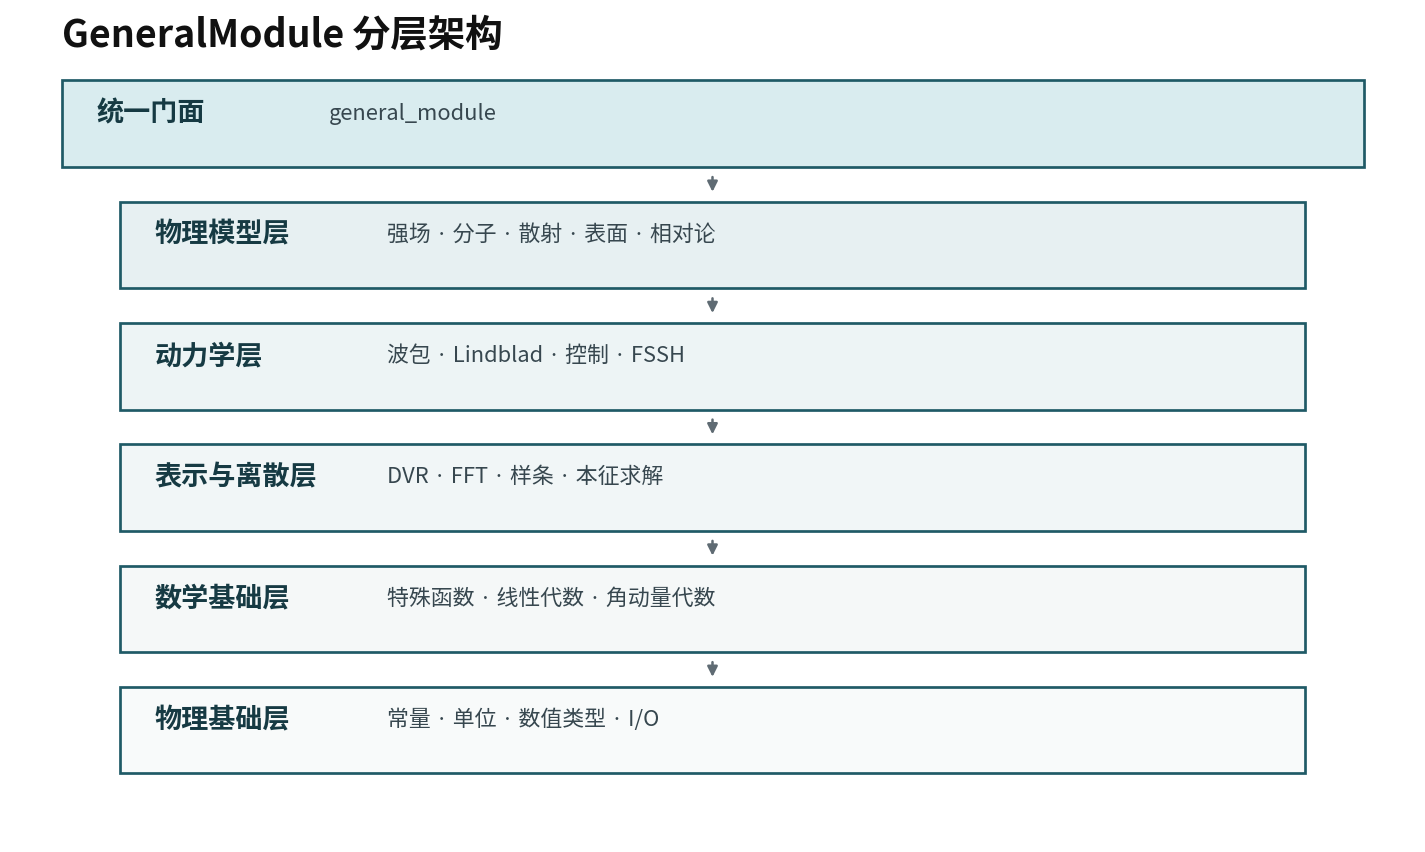
\includegraphics[width=5.98425in,height=3.57795in]{media/image1.png}

图 1-1 GeneralModule 的分层架构与依赖方向

\textbf{表 1-1 项目分层与教学重点}

\begin{longtable}[]{@{}llll@{}}
\toprule
\textbf{层级} & \textbf{代表模块} & \textbf{主要职责} &
\textbf{学习重点}\tabularnewline
\midrule
\endhead
物理基础 & mod\_constants, mod\_io\_utils & 类型、常量、单位、输入输出 &
单位契约与数值精度\tabularnewline
数学基础 & mod\_special\_functions, mod\_linear\_algebra &
特殊函数、本征、FFT、矩阵求逆 & 算法假设与自洽性\tabularnewline
表示与离散 & mod\_dvr\_grid, mod\_interpolation &
DVR、FGH、样条与势能面外推 & 离散表象与边界误差\tabularnewline
动力学 & mod\_wavepacket\_propagator, mod\_open\_quantum &
波包、RK4、ABM4、Lindblad & 稳定性、守恒与收敛\tabularnewline
物理模型 & mod\_ti\_scattering, mod\_field\_scattering 等 &
散射、强场、表面、相对论 & 边界匹配与物理量解释\tabularnewline
用户接口 & general\_module & 统一 re-export & API
可见性与版本管理\tabularnewline
\bottomrule
\end{longtable}

\section{\texorpdfstring{\textbf{1.1 统一门面
general\_module}}{1.1 统一门面 general\_module}}\label{ux7edfux4e00ux95e8ux9762-general_module}

general\_module 不是主程序，而是聚合模块。它通过 use 重新导出 49
个核心模块中的公共实体，使用户只需写一行 use general\_module
即可访问大部分 API。示例 ex01 正是这样开始：

\textbf{代码 1-1 通过统一门面访问 DVR
类型（examples/ex01\_fgh\_diatomic\_bound\_states.f90:2-6）}

\begin{quote}
program ex01\_fgh\_diatomic\_bound\_states\\
use general\_module\\
implicit none\\
type(dvr\_1d\_t) :: dvr
\end{quote}

\begin{longtable}[]{@{}l@{}}
\toprule
\endhead
\begin{minipage}[t]{0.97\columnwidth}\raggedright
\textbf{设计原则}

general\_module 适合作为用户 API
门面，不应成为低层模块的内部依赖。保持单向依赖可以避免循环依赖，并让单独测试某个基础模块成为可能。\strut
\end{minipage}\tabularnewline
\bottomrule
\end{longtable}

\section{\texorpdfstring{\textbf{1.2 现代 Fortran
工程特征}}{1.2 现代 Fortran 工程特征}}\label{ux73b0ux4ee3-fortran-ux5de5ux7a0bux7279ux5f81}

\begin{itemize}
\item
  \begin{quote}
  所有主要源文件使用 implicit none，关闭隐式类型和隐式外部声明。
  \end{quote}
\item
  \begin{quote}
  过程参数使用 intent(in)、intent(out)、intent(inout) 明确副作用。
  \end{quote}
\item
  \begin{quote}
  大量数学过程标记为 pure，支持编译器优化与可复现推理。
  \end{quote}
\item
  \begin{quote}
  动态输出使用 allocatable；配置与结果通过派生类型封装。
  \end{quote}
\item
  \begin{quote}
  模块默认 private，再以 public 列表形成显式白名单。
  \end{quote}
\end{itemize}

\section{\texorpdfstring{\textbf{1.3
如何阅读一个大型科学库}}{1.3 如何阅读一个大型科学库}}\label{ux5982ux4f55ux9605ux8bfbux4e00ux4e2aux5927ux578bux79d1ux5b66ux5e93}

\begin{quote}
1. 先读模块头注释，确认方程、单位、输入输出和算法名称。

2. 再读派生类型，判断哪些量是配置、哪些量是结果、哪些数组在运行时分配。

3. 沿依赖关系向下追踪基础函数，而不是只沿目录顺序阅读。

4. 把对应测试和示例当作可执行规格；它们揭示了作者真正关心的不变量。

5. 最后检查文档数量、文件数量和实现是否一致，把版本残留记录为维护任务。
\end{quote}

\begin{longtable}[]{@{}l@{}}
\toprule
\endhead
\begin{minipage}[t]{0.97\columnwidth}\raggedright
\textbf{练习 1-1 架构阅读}

\begin{quote}
1. 画出 mod\_dvr\_grid、mod\_wavepacket\_propagator 和 general\_module
的依赖关系。

2. 找出至少四个使用派生类型作为配置或结果容器的模块。

3. 解释为什么聚合模块不应被底层求解器使用。
\end{quote}\strut
\end{minipage}\tabularnewline
\bottomrule
\end{longtable}

\chapter{第2章 Fortran 2008 科学计算基础}\label{ux7b2c2ux7ae0-fortran-2008-ux79d1ux5b66ux8ba1ux7b97ux57faux7840}

本章把项目中反复出现的 Fortran
机制串成一套可迁移的工程习惯。重点不是语法大全，而是如何让科学计算的接口可检查、结果可复现、错误可定位。

\section{\texorpdfstring{\textbf{2.1
模块、可见性与类型别名}}{2.1 模块、可见性与类型别名}}\label{ux6a21ux5757ux53efux89c1ux6027ux4e0eux7c7bux578bux522bux540d}

\textbf{代码 2-1 数值类型与可见性（src/mod\_constants.f90:3-22）}

\begin{quote}
module mod\_constants\\
use, intrinsic :: iso\_fortran\_env, only: dp =\textgreater{} real64,
int32, int64\\
implicit none\\
private\\
public :: dp, int32, int64\\
public :: to\_au, from\_au
\end{quote}

dp 是 real64 的项目级别名。把精度策略集中在
mod\_constants，可以避免各模块各自选择 real 或 double
precision。整数类型 int32 与 int64
则适合数组索引、位运算和需要明确位宽的元数据。

\section{\texorpdfstring{\textbf{2.2
intent：把副作用写进接口}}{2.2 intent：把副作用写进接口}}\label{intentux628aux526fux4f5cux7528ux5199ux8fdbux63a5ux53e3}

\begin{quote}
纯函数：f(x) → y

输入 intent(in)，结果由 function result 返回；可安全标记 pure。

原地更新：subroutine step(y, dt)

y 使用 intent(inout)，调用方立即知道对象会被修改。

独立输出：subroutine solve(..., result, stat)

result 与 stat 使用 intent(out)，避免隐藏的全局状态。
\end{quote}

项目大量把状态码设计为可选 intent(out)
参数。例如散射长度计算在网格过短时把 stat 设为 -1；这比直接 stop
更适合作为库函数，因为库不应替用户决定进程退出。

\section{\texorpdfstring{\textbf{2.3 allocatable
与派生类型}}{2.3 allocatable 与派生类型}}\label{allocatable-ux4e0eux6d3eux751fux7c7bux578b}

\textbf{代码 2-2
将网格与动能矩阵封装为对象（src/mod\_dvr\_grid.f90:17-26）}

\begin{quote}
type :: dvr\_1d\_t\\
integer :: n\_points = 0\\
real(dp) :: dx = 0.0\_dp\\
real(dp), allocatable :: x(:)\\
real(dp), allocatable :: t\_mat(:, :)\\
end type dvr\_1d\_t
\end{quote}

派生类型把物理配置、运行时数组与算法状态放在同一对象中。调用者不需要维护一长串相互关联的实参数。代价是对象复制可能带来深拷贝成本，因此大矩阵通常在
init 或 solve 阶段分配，而不是在高频循环中反复赋值。

\section{\texorpdfstring{\textbf{2.4
过程接口与回调}}{2.4 过程接口与回调}}\label{ux8fc7ux7a0bux63a5ux53e3ux4e0eux56deux8c03}

rk4\_step 和 abm4\_step 使用过程内 interface
声明纯导数函数。通用积分器因此不需要知道被积系统的物理细节。回调接口让测试变得直接：可以传入解析导数、常数系统或人为构造的刚性系统。

\textbf{代码 2-3
显式过程接口（src/mod\_wavepacket\_propagator.f90:80-90）}

\begin{quote}
interface\\
pure function f\_deriv(t\_in, y\_in) result(dydt)\\
real(dp), intent(in) :: t\_in, y\_in(:)\\
real(dp) :: dydt(size(y\_in))\\
end function f\_deriv\\
end interface
\end{quote}

\begin{longtable}[]{@{}l@{}}
\toprule
\endhead
\begin{minipage}[t]{0.97\columnwidth}\raggedright
\textbf{常见错误}

Fortran 默认是按引用传递。若一个只想读取的数组漏写
intent(in)，过程仍可能意外修改调用者数据。编译器通常不会替你修正接口契约。\strut
\end{minipage}\tabularnewline
\bottomrule
\end{longtable}

\begin{longtable}[]{@{}l@{}}
\toprule
\endhead
\begin{minipage}[t]{0.97\columnwidth}\raggedright
\textbf{练习 2-1 接口审查}

\begin{quote}
1. 为 calculate\_von\_neumann\_entropy 的每个参数判断 intent 是否合理。

2. 找出项目中返回 allocatable 结果的过程，说明为什么不能简单写成
intent(out)。

3. 解释 pure procedure 为什么不能直接写文件或修改全局变量。
\end{quote}\strut
\end{minipage}\tabularnewline
\bottomrule
\end{longtable}

\chapter{第3章 单位、常数与数值安全}\label{ux7b2c3ux7ae0-ux5355ux4f4dux5e38ux6570ux4e0eux6570ux503cux5b89ux5168}

量子动力学计算经常在原子单位、实验单位和高斯---厘米制之间切换。单位错误不会像语法错误那样容易被编译器发现，却可能让结果相差若干个数量级。mod\_constants
因此不仅是常数表，更是整个库的物理语义入口。

\section{\texorpdfstring{\textbf{3.1
原子单位与实验单位}}{3.1 原子单位与实验单位}}\label{ux539fux5b50ux5355ux4f4dux4e0eux5b9eux9a8cux5355ux4f4d}

\textbf{表 3-1 mod\_constants 中的代表性单位接口}

\begin{longtable}[]{@{}lll@{}}
\toprule
\textbf{量} & \textbf{项目符号} & \textbf{换算含义}\tabularnewline
\midrule
\endhead
时间 & AU2FS, FS2AU & 1 a.u. 时间与飞秒互换\tabularnewline
能量 & AU2EV, AU2CM, AU2K & Hartree 与 eV、cm⁻¹、K 互换\tabularnewline
长度 & AU2ANG, AU2NM, AU2M & Bohr 与 Å、nm、m 互换\tabularnewline
电场 & AU2VM, AU2MV\_CM & 原子单位电场与 V/m、MV/cm 互换\tabularnewline
磁场 & AU2TESLA, AU2GAUSS & 原子单位磁场与 T、G 互换\tabularnewline
\bottomrule
\end{longtable}

\section{\texorpdfstring{\textbf{3.2
字符串分派接口}}{3.2 字符串分派接口}}\label{ux5b57ux7b26ux4e32ux5206ux6d3eux63a5ux53e3}

\textbf{代码 3-1 单位字符串分派（src/mod\_constants.f90:90-133，节选）}

\begin{quote}
pure function to\_au(val, unit\_name) result(val\_au)\\
real(dp), intent(in) :: val\\
character(len=*), intent(in) :: unit\_name\\
real(dp) :: val\_au\\
~\\
select case (trim(adjustl(unit\_name)))\\
case ('fs')\\
val\_au = val * FS2AU\\
case ('ev', 'eV')\\
val\_au = val * EV2AU\\
case default\\
val\_au = val\\
end select\\
end function to\_au
\end{quote}

字符串接口对教学示例很友好：用户不必记住每个转换因子的名字。但 default
分支直接返回原值，意味着未知单位不会报错。对于脚本或交互式示例，这种容错可能方便；对于长期计算，它可能掩盖拼写错误。更严格的方案是增加
status 输出或使用领域特定强类型单位。

\begin{longtable}[]{@{}l@{}}
\toprule
\endhead
\begin{minipage}[t]{0.97\columnwidth}\raggedright
\textbf{安全建议}

在生产流程中记录原始单位、目标单位和转换函数；不要只记录转换后的数字。未知单位应显式失败，而不是静默通过。\strut
\end{minipage}\tabularnewline
\bottomrule
\end{longtable}

\section{\texorpdfstring{\textbf{3.3
数值精度与极端尺度}}{3.3 数值精度与极端尺度}}\label{ux6570ux503cux7cbeux5ea6ux4e0eux6781ux7aefux5c3aux5ea6}

项目使用双精度 real64
作为默认实数。强场和散射问题仍可能出现大动态范围：深势阱内指数增长、外边界长距离传播、极小非零初值、矩阵元素相差多个数量级。阅读数值代码时，应主动寻找重缩放、对数导数、log-space
或条件分支。

\textbf{代码 3-2 Numerov
传播中的重缩放（src/mod\_ti\_scattering.f90:246-249）}

\begin{quote}
if (abs(u\_wf(i + 1)) \textgreater{} 1.0e20\_dp) then\\
u\_wf(1:i + 1) = u\_wf(1:i + 1) * 1.0e-15\_dp\\
end if
\end{quote}

\begin{longtable}[]{@{}l@{}}
\toprule
\endhead
\begin{minipage}[t]{0.97\columnwidth}\raggedright
\textbf{练习 3-1 单位审计}

\begin{quote}
1. 为一段包含 fs、eV、angstrom 的输入建立单位追踪表。

2. 找出所有会静默返回原值的单位接口调用。

3. 设计一个 status 输出版本的 to\_au，并说明它对自动化测试的价值。
\end{quote}\strut
\end{minipage}\tabularnewline
\bottomrule
\end{longtable}

\chapter{第4章 特殊函数、矩阵算法与自包含数值核心}\label{ux7b2c4ux7ae0-ux7279ux6b8aux51fdux6570ux77e9ux9635ux7b97ux6cd5ux4e0eux81eaux5305ux542bux6570ux503cux6838ux5fc3}

GeneralModule
的一个显著特征是：核心数值能力主要由项目内部实现，而不是强制依赖
LAPACK、BLAS 或
FFTW。这提高了部署便携性，但也把算法正确性、维数支持和边界条件审查的责任放回项目内部。

\section{\texorpdfstring{\textbf{4.1
特殊函数与角动量代数}}{4.1 特殊函数与角动量代数}}\label{ux7279ux6b8aux51fdux6570ux4e0eux89d2ux52a8ux91cfux4ee3ux6570}

mod\_special\_functions 提供 Legendre 多项式、缔合勒让德函数、Wigner
3j、Clebsch--Gordan 系数、半整数角动量版本、Wigner 6j/9j
与转动偶极矩阵元。角动量算法的核心不是``算出系数''，而是同时满足选择定则、对称性和归一化关系。

\begin{quote}
j₁ + j₂ + J ≥ \textbar j₁ − j₂\textbar, \textbar m₁ − m₂\textbar{} ≤ M ≤
\textbar m₁ + m₂\textbar{}

三角定则与磁量子数定则应在测试中作为硬约束检查。
\end{quote}

\section{\texorpdfstring{\textbf{4.2
实对称矩阵本征求解}}{4.2 实对称矩阵本征求解}}\label{ux5b9eux5bf9ux79f0ux77e9ux9635ux672cux5f81ux6c42ux89e3}

mod\_linear\_algebra 组合 Householder 三对角化与隐式位移 QL
迭代，求解实对称矩阵的本征值和本征向量。FGH、开放量子系统熵和许多二能级模型都依赖这一基础设施。

\textbf{算法 4-1 项目内部实对称本征求解流程}

\begin{quote}
输入实对称矩阵 A\\
↓ Householder 三对角化\\
三对角矩阵 T = QᵀAQ\\
↓ 隐式位移 QL 迭代\\
本征值 diag(Λ) 与本征向量 Q 的列向量
\end{quote}

\section{\texorpdfstring{\textbf{4.3 FFT 与非 2
的幂长度}}{4.3 FFT 与非 2 的幂长度}}\label{fft-ux4e0eux975e-2-ux7684ux5e42ux957fux5ea6}

内部 FFT 采用位反转重排和蝶形运算。对非 2 的幂长度，代码回退到较慢的
DFT。这是一种清晰且可移植的工程折中：牺牲非标准长度的性能，保持核心库不依赖外部
FFT。

\textbf{表 4-1 数值线性代数能力与风险}

\begin{longtable}[]{@{}llll@{}}
\toprule
\textbf{算法} & \textbf{适用问题} & \textbf{主要风险} &
\textbf{项目对策}\tabularnewline
\midrule
\endhead
Householder + QL & 实对称本征 & 实现细节多、重复本征值 &
测试与对称矩阵对照\tabularnewline
FFT & 周期域卷积、动量表象 & 长度与归一化、边界周期 & 位反转 +
逆变换归一化\tabularnewline
DFT fallback & 非 2 的幂长度 & 复杂度 O(N²) &
保留正确性，明确性能代价\tabularnewline
Gauss-Jordan & 矩阵求逆 & 条件数、近奇异 &
状态码与奇异检测\tabularnewline
\bottomrule
\end{longtable}

\begin{longtable}[]{@{}l@{}}
\toprule
\endhead
\begin{minipage}[t]{0.97\columnwidth}\raggedright
\textbf{选择定则}

任何本征求解器都至少应测试：3×3
对角阵、随机实对称阵、重复本征值、单位矩阵、负定矩阵和已知解析旋转矩阵。\strut
\end{minipage}\tabularnewline
\bottomrule
\end{longtable}

\begin{longtable}[]{@{}l@{}}
\toprule
\endhead
\begin{minipage}[t]{0.97\columnwidth}\raggedright
\textbf{练习 4-1 数值线性代数}

\begin{quote}
1. 构造含重复本征值的对角阵，验证本征向量归一化。

2. 比较 2 的幂与非 2 的幂长度 FFT 的结果。

3. 为矩阵求逆构造接近奇异的矩阵，记录状态码与残差。
\end{quote}\strut
\end{minipage}\tabularnewline
\bottomrule
\end{longtable}

\chapter{第5章 DVR、FGH 与束缚态}\label{ux7b2c5ux7ae0-dvrfgh-ux4e0eux675fux7f1aux6001}

离散变量表象（DVR）把局域坐标表象转换为适合矩阵本征求解的有限维表示。对分子振动态，势能在网格点上是局域的，而动能变成稠密矩阵。FGH（Fourier
Grid Hamiltonian）正是 T + V 的离散实现。

\section{\texorpdfstring{\textbf{5.1 Sinc-DVR
网格}}{5.1 Sinc-DVR 网格}}\label{sinc-dvr-ux7f51ux683c}

\textbf{代码 5-1 Sinc-DVR
动能矩阵构造（src/mod\_dvr\_grid.f90:65-85，节选）}

\begin{quote}
dvr\%dx = (x\_max - x\_min) / real(n\_pts + 1, dp)\\
~\\
factor = 1.0\_dp / (2.0\_dp * mass * dvr\%dx**2)\\
do i = 1, n\_pts\\
do j = 1, n\_pts\\
if (i == j) then\\
dvr\%t\_mat(i, j) = factor * (PI**2 / 3.0\_dp)\\
else\\
diff\_sq = real((i - j)**2, dp)\\
if (mod(i - j, 2) == 0) then\\
dvr\%t\_mat(i, j) = factor * (2.0\_dp / diff\_sq)\\
else\\
dvr\%t\_mat(i, j) = -factor * (2.0\_dp / diff\_sq)\\
end if\\
end if\\
end do\\
end do
\end{quote}

\section{\texorpdfstring{\textbf{5.2 FGH
矩阵与归一化}}{5.2 FGH 矩阵与归一化}}\label{fgh-ux77e9ux9635ux4e0eux5f52ux4e00ux5316}

\begin{quote}
Hᵢⱼ = Tᵢⱼ + V(xᵢ)δᵢⱼ

势能只在 DVR 网格上对角化；动能一般是非对角矩阵。
\end{quote}

项目在求解后通过 ψ(xᵢ)=eig\_vecs(i,v)/sqrt(dx)
完成连续坐标归一化。任何直接使用 eig\_vecs
的代码都必须明确它究竟是离散归一化向量还是坐标表象波函数。

\section{\texorpdfstring{\textbf{5.3 ex01：Morse
束缚态完整案例}}{5.3 ex01：Morse 束缚态完整案例}}\label{ex01morse-ux675fux7f1aux6001ux5b8cux6574ux6848ux4f8b}

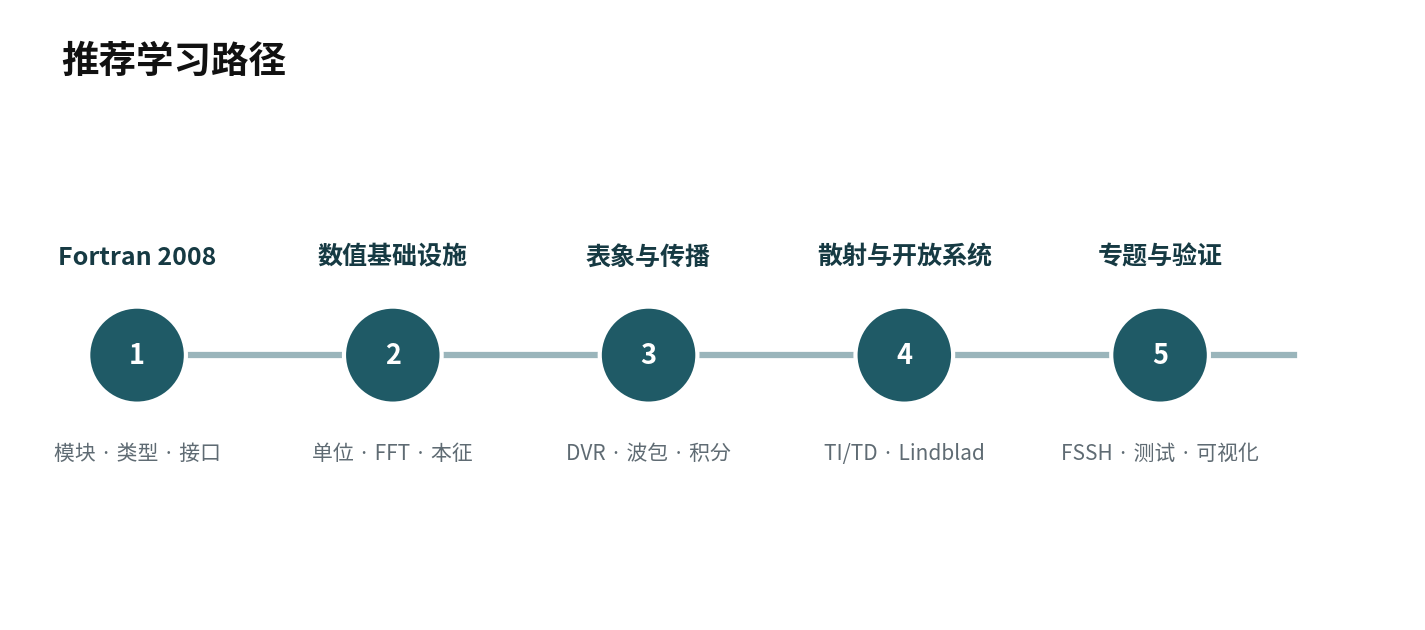
\includegraphics[width=5.98425in,height=2.64567in]{media/image2.png}

图 5-1 推荐的渐进学习路径

\begin{quote}
1. 设置 Dₑ、Rₑ、β 与约化质量 μ。

2. 初始化 0.8---6.0 Bohr、256 点的 Sinc-DVR。

3. 在网格上构造 Morse 势 V(R)=Dₑ{[}1−exp(−β(R−Rₑ)){]}²。

4. 调用 fgh\_solve\_bound\_states 对角化 H。

5. 将前六个能级与 Morse 解析公式比较。

6. 导出基态与前三个激发态波函数。
\end{quote}

\textbf{代码 5-2
从势能到本征态的调用链（examples/ex01\_fgh\_diatomic\_bound\_states.f90:32-48，节选）}

\begin{quote}
call dvr\_sinc\_init(r\_min, r\_max, n\_pts, mu\_mass, dvr)\\
~\\
do i = 1, n\_pts\\
v\_morse(i) = d\_e * \&\\
(1.0\_dp - exp(-beta * (dvr\%x(i) - r\_e)))**2\\
end do\\
~\\
call fgh\_solve\_bound\_states(dvr, v\_morse, eig\_vals, eig\_vecs,
stat)
\end{quote}

\begin{longtable}[]{@{}l@{}}
\toprule
\endhead
\begin{minipage}[t]{0.97\columnwidth}\raggedright
\textbf{收敛性实验}

依次把网格从 128、256、512、1024
点增加，并同时调整区间和步长。只有能级、波函数和范数都稳定，数值结果才可进入下一阶段。\strut
\end{minipage}\tabularnewline
\bottomrule
\end{longtable}

\begin{longtable}[]{@{}l@{}}
\toprule
\endhead
\begin{minipage}[t]{0.97\columnwidth}\raggedright
\textbf{练习 5-1 FGH}

\begin{quote}
1. 复现 ex01 并记录前六个能级随 n\_pts 的变化。

2. 缩小和扩大积分区间，判断边界反射对高振动态的影响。

3. 把 Morse 势替换为谐振子势，比较能级误差。
\end{quote}\strut
\end{minipage}\tabularnewline
\bottomrule
\end{longtable}

\chapter{第6章 波包传播、积分器与吸收边界}\label{ux7b2c6ux7ae0-ux6ce2ux5305ux4f20ux64adux79efux5206ux5668ux4e0eux5438ux6536ux8fb9ux754c}

含时量子动力学常把演化写成线性演化元作用于初态。分裂算符法利用动能在动量表象对角、势能在坐标表象对角，通过
FFT 在两个表象之间切换。

\section{\texorpdfstring{\textbf{6.1 Split-Operator
五步法}}{6.1 Split-Operator 五步法}}\label{split-operator-ux4e94ux6b65ux6cd5}

\begin{quote}
ψ(t+dt) = e\^{}(−iVdt/2) IFFT \{ e\^{}(−iTdt) FFT {[} e\^{}(−iVdt/2)
ψ(t) {]} \}

1. 在坐标表象施加势能半步相位。

2. FFT 变换到动量表象。

3. 施加动能整步相位。

4. IFFT 返回坐标表象。

5. 再次施加势能半步相位。
\end{quote}

这种对称分裂在理想情况下保持范数，因为每个子步骤都是酉变换。真正破坏守恒的来源通常包括：离散
FFT 归一化、吸收边界、过大时间步、复势处理和后处理归一化。

\section{\texorpdfstring{\textbf{6.2 RK4 与
ABM4}}{6.2 RK4 与 ABM4}}\label{rk4-ux4e0e-abm4}

RK4 每次推进需要四次导数评估，局部误差通常为 O(dt⁵)。ABM4
使用过去三个导数和当前导数做 Adams--Bashforth
四阶预估，再在预估点计算导数，用 Adams--Moulton
四阶公式校正。多步法的效率更高，但需要一致的启动策略和历史导数缓存。

\begin{longtable}[]{@{}l@{}}
\toprule
\endhead
\begin{minipage}[t]{0.97\columnwidth}\raggedright
\textbf{多步法检查}

多步法不应只测试``能运行''。需要检查阶数、步长缩放、历史缓存错位、非光滑右端项和长时间漂移。\strut
\end{minipage}\tabularnewline
\bottomrule
\end{longtable}

\section{\texorpdfstring{\textbf{6.3 CAP
与开放边界}}{6.3 CAP 与开放边界}}\label{cap-ux4e0eux5f00ux653eux8fb9ux754c}

mod\_absorbing\_boundary 提供 sin² CAP、多项式
CAP、概率流和内部区域范数。CAP
通过虚势让离开内部计算区域的波包指数衰减，避免硬壁造成非物理反射。

\begin{longtable}[]{@{}l@{}}
\toprule
\endhead
\begin{minipage}[t]{0.97\columnwidth}\raggedright
\textbf{练习 6-1 波包}

\begin{quote}
1. 对无外场自由粒子波包运行 Split-Operator，监测位置和动量期望值。

2. 逐步减小 dt，验证范数误差随步长快速下降。

3. 在网格边缘加入 CAP，比较边界反射和吸收时间。
\end{quote}\strut
\end{minipage}\tabularnewline
\bottomrule
\end{longtable}

\chapter{第7章 激光脉冲、热平均与强场物理}\label{ux7b2c7ux7ae0-ux6fc0ux5149ux8109ux51b2ux70edux5e73ux5747ux4e0eux5f3aux573aux7269ux7406}

强场物理把数值波包、激光脉冲、原子势和频率域观测连接起来。项目提供高斯、sin²、啁啾、双色和
THz 脉冲配置，以及库仑原子、ADK、HHG 与频谱模块。

\section{\texorpdfstring{\textbf{7.1
脉冲配置对象}}{7.1 脉冲配置对象}}\label{ux8109ux51b2ux914dux7f6eux5bf9ux8c61}

pulse\_config\_t
将中心频率、带宽、时间包络、偏振和传播参数封装成对象。相比把每个参数作为位置实参，配置对象更容易扩展，也更适合示例程序表达物理意图。

\section{\texorpdfstring{\textbf{7.2
热系综}}{7.2 热系综}}\label{ux70edux7cfbux7efc}

\begin{quote}
w\_J = (2J+1)e\^{}(−βBJ(J+1)) / Z\_rot

转动布居同时包含简并度和玻尔兹曼因子。
\end{quote}

热平均不能只对单个代表性 J
做计算，而应在适当归一化的权重上求和。振动系综和 Bose--Einstein
因子也遵循同样原则：先定义物理统计分布，再计算可观测量。

\section{\texorpdfstring{\textbf{7.3
从时域到频域}}{7.3 从时域到频域}}\label{ux4eceux65f6ux57dfux5230ux9891ux57df}

HHG、光碎片谱和瞬态吸收都需要从时域相关函数或偶极矩得到频谱。谱方法的关键不只是
FFT，还包括时间窗、采样长度、零填充和相干性。有限时间窗会造成谱泄漏；Hanning
窗可降低旁瓣，但同时牺牲分辨率。

\begin{longtable}[]{@{}l@{}}
\toprule
\endhead
\begin{minipage}[t]{0.97\columnwidth}\raggedright
\textbf{练习 7-1 强场模块}

\begin{quote}
1. 构造 Gaussian 与 sin² 脉冲，比较峰值场强和频谱宽度。

2. 验证热平均权重归一化，并比较不同温度下的布居。

3. 改变谱计算时间窗，观察分辨率与泄漏的折中。
\end{quote}\strut
\end{minipage}\tabularnewline
\bottomrule
\end{longtable}

\chapter{第8章 非含时散射：Numerov、对数导数与 S 矩阵}\label{ux7b2c8ux7ae0-ux975eux542bux65f6ux6563ux5c04numerovux5bf9ux6570ux5bfcux6570ux4e0e-s-ux77e9ux9635}

定态散射模块是项目最完整、最值得系统学习的算法模块之一。它同时包含特殊渐近函数、零能散射长度、有限能分波相移、截面、光学定理、有效力程、共振、多通道密耦和分段网格。

\section{\texorpdfstring{\textbf{8.1
零能方程与散射长度}}{8.1 零能方程与散射长度}}\label{ux96f6ux80fdux65b9ux7a0bux4e0eux6563ux5c04ux957fux5ea6}

\begin{quote}
−(ℏ²/2μ)u″(r) + V(r)u(r) = 0\\
零能渐近：u(r) → C(r−aₛ)
\end{quote}

Numerov
方法用多点递推提高二阶方程的离散精度。与简单三点差分相比，它对光滑势函数的相移误差更小，但需要合理网格和更谨慎的边界区域。

\textbf{代码 8-1 Numerov
递推（src/mod\_ti\_scattering.f90:233-245，节选）}

\begin{quote}
do i = 2, n\_pts - 1\\
q\_prev = -2.0\_dp * mass * v\_pot(i - 1)\\
q\_curr = -2.0\_dp * mass * v\_pot(i)\\
q\_next = -2.0\_dp * mass * v\_pot(i + 1)\\
~\\
c\_prev = 1.0\_dp + dr2\_12 * q\_prev\\
c\_curr = 2.0\_dp * (1.0\_dp - 5.0\_dp * dr2\_12 * q\_curr)\\
c\_next = 1.0\_dp + dr2\_12 * q\_next\\
~\\
u\_wf(i + 1) = (c\_curr*u\_wf(i) - c\_prev*u\_wf(i-1)) / c\_next\\
end do
\end{quote}

\section{\texorpdfstring{\textbf{8.2 Johnson
对数导数比值法}}{8.2 Johnson 对数导数比值法}}\label{johnson-ux5bf9ux6570ux5bfcux6570ux6bd4ux503cux6cd5}

直接传播 u 容易在深势阱中指数溢出。Johnson 方法传播相邻点比值
Rᵢ=uᵢ/uᵢ₋₁，把绝对幅值消掉，因此对深势阱更稳定。项目在零能散射长度接口中直接实现了这一递推。

\begin{quote}
Rᵢ₊₁ = {[}2(1−5wᵢ) − (1+wᵢ₋₁)/Rᵢ{]} / (1+wᵢ₊₁)
\end{quote}

\section{\texorpdfstring{\textbf{8.3
渐近匹配与相移}}{8.3 渐近匹配与相移}}\label{ux6e10ux8fd1ux5339ux914dux4e0eux76f8ux79fb}

有限能分波在匹配半径 R 处把数值解与 Riccati--Bessel/Neumann
渐近函数组合，由外边界对数导数和相位信息得到 δₗ。随后
Sₗ=exp(2iδₗ)、Kₗ=tan(δₗ)、Tₗ=Sₗ−1 形成相互校验的物理量。

\section{\texorpdfstring{\textbf{8.4
交叉验证策略}}{8.4 交叉验证策略}}\label{ux4ea4ux53c9ux9a8cux8bc1ux7b56ux7565}

\begin{quote}
1. 同一势能同时用 Numerov 与 Log-Derivative 计算散射长度。

2. 对无相互作用势验证 δₗ=0、Sₗ=1、σ=0。

3. 验证光学定理和总截面的一致性。

4. 在匹配半径、网格密度和入射能附近做收敛扫描。

5. 用已知解析平方阱或方势垒进行定量对照。
\end{quote}

\begin{longtable}[]{@{}l@{}}
\toprule
\endhead
\begin{minipage}[t]{0.97\columnwidth}\raggedright
\textbf{命名核查}

mod\_ti\_scattering 中个别名为``矩阵
Numerov''的耦合推进，表达式外观更接近显式矩阵差分。教材不据此断言算法错误，但建议通过收敛阶测试和文献对照确认名称与实现。\strut
\end{minipage}\tabularnewline
\bottomrule
\end{longtable}

\begin{longtable}[]{@{}l@{}}
\toprule
\endhead
\begin{minipage}[t]{0.97\columnwidth}\raggedright
\textbf{练习 8-1 散射长度}

\begin{quote}
1. 对无相互作用 V=0 验证 aₛ 的数值行为。

2. 比较 Numerov 与 Log-Derivative 在不同网格和势深下的结果。

3. 对形状共振扫描 Sₗ，并提取 Wigner 时延。
\end{quote}\strut
\end{minipage}\tabularnewline
\bottomrule
\end{longtable}

\chapter{第9章 含时散射、多通道与 Feshbach 共振}\label{ux7b2c9ux7ae0-ux542bux65f6ux6563ux5c04ux591aux901aux9053ux4e0e-feshbach-ux5171ux632f}

含时波包散射用时间域传播获得透射、反射和谱信息；定态多通道散射则直接构造
S 矩阵。两者可以互相验证：稳态概率流应与波包累积通量一致。

\section{\texorpdfstring{\textbf{9.1
高斯波包与通量累积}}{9.1 高斯波包与通量累积}}\label{ux9ad8ux65afux6ce2ux5305ux4e0eux901aux91cfux7d2fux79ef}

mod\_td\_scattering
提供高斯初态波包、动量振幅、时间---能量通量、透射率、S 矩阵元、Wigner
延迟和二维微分散射截面。含时方法直观但对初态宽度、脉冲长度和能量分辨率敏感。

\section{\texorpdfstring{\textbf{9.2
多通道密耦}}{9.2 多通道密耦}}\label{ux591aux901aux9053ux5bc6ux8026}

多通道散射需要传播矩阵 Riccati
变量或矩阵对数导数，区分开通道与闭通道，并在耦合矩阵非对角时保持数值稳定。结果对象
multichannel\_result\_t 包含 K、S、T、跃迁概率、分截面与特征相移和。

\begin{quote}
S = (I + iK)(I − iK)⁻¹

这是由实对称 K 矩阵得到严格幺正 S 矩阵的 Cayley 变换。
\end{quote}

\section{\texorpdfstring{\textbf{9.3 Breit--Rabi 基组与 Feshbach
扫描}}{9.3 Breit--Rabi 基组与 Feshbach 扫描}}\label{breitrabi-ux57faux7ec4ux4e0e-feshbach-ux626bux63cf}

mod\_field\_scattering
提供非耦合、超精细、总自旋耦合和场缀饰渐近通道基组。磁场扫描的核心流程是：给定
B，构造通道本征态和渐近投影，调用多通道
Log-Derivative，提取入射道散射长度 aₛ(B)，再拟合共振参数。

\begin{quote}
aₛ(B) = a\_bg {[}1 − ΔB/(B − B₀){]}
\end{quote}

\textbf{表 9-1 Feshbach 计算链}

\begin{longtable}[]{@{}llll@{}}
\toprule
\textbf{阶段} & \textbf{主要输入} & \textbf{主要输出} &
\textbf{失败信号}\tabularnewline
\midrule
\endhead
基组构造 & 电子自旋、磁场、通道阈值 & 通道向量与投影 &
正交性或阈值异常\tabularnewline
径向密耦 & 势矩阵、E、l、网格 & K/S/T 与截面 & S
非幺正、状态码失败\tabularnewline
外场扫描 & B 范围与步长 & aₛ(B) 数据 & 奇异点、拟合失败\tabularnewline
共振拟合 & B₀、ΔB、a\_bg & 共振参数 &
残差大、置信区间异常\tabularnewline
\bottomrule
\end{longtable}

\begin{longtable}[]{@{}l@{}}
\toprule
\endhead
\begin{minipage}[t]{0.97\columnwidth}\raggedright
\textbf{练习 9-1 多通道}

\begin{quote}
1. 构造两个弱耦合通道，验证无耦合极限 S→I。

2. 检查 S 矩阵幺正性并计算最大模残差。

3. 对二维参数空间扫描 aₛ(B)，拟合 Feshbach 共振。
\end{quote}\strut
\end{minipage}\tabularnewline
\bottomrule
\end{longtable}

\chapter{第10章 开放量子系统与量子控制}\label{ux7b2c10ux7ae0-ux5f00ux653eux91cfux5b50ux7cfbux7edfux4e0eux91cfux5b50ux63a7ux5236}

封闭量子系统用波函数或纯态传播；与环境耦合后通常需要密度矩阵。mod\_open\_quantum
以 Lindblad 主方程为基础，提供弛豫与退相位 Jump 算符、RK4
推进、纯度、相干度和熵。

\section{\texorpdfstring{\textbf{10.1 Jump
算符与耗散项}}{10.1 Jump 算符与耗散项}}\label{jump-ux7b97ux7b26ux4e0eux8017ux6563ux9879}

\begin{quote}
D{[}L{]}ρ = LρL† − ½(L†Lρ + ρL†L)
\end{quote}

\textbf{代码 10-1 Lindblad
耗散超算符（src/mod\_open\_quantum.f90:54-63，节选）}

\begin{quote}
l\_dag = conjg(transpose(l\_op))\\
l\_dag\_l = matmul(l\_dag, l\_op)\\
~\\
term1 = matmul(l\_op, matmul(rho, l\_dag))\\
term2 = matmul(l\_dag\_l, rho)\\
term3 = matmul(rho, l\_dag\_l)\\
~\\
d\_rho = term1 - 0.5\_dp * (term2 + term3)
\end{quote}

\section{\texorpdfstring{\textbf{10.2
数值守恒}}{10.2 数值守恒}}\label{ux6570ux503cux5b88ux6052}

RK4
更新后，代码显式对称化密度矩阵并重新归一化迹。这能抑制有限步长造成的厄米性和迹误差，但也可能掩盖过大的
dt。正确做法是同时监测更新前后的厄米残差、迹误差和正定性，不要只依赖事后修正。

\section{\texorpdfstring{\textbf{10.3
诊断量}}{10.3 诊断量}}\label{ux8bcaux65adux91cf}

\begin{quote}
Purity = Tr(ρ²), S = −Tr(ρ ln ρ)
\end{quote}

纯度反映混合程度，相干度反映非对角矩阵元，熵反映信息扩散。三者应与布居转移、受激辐射和退相位速率形成一致的时间演化图景。

\section{\texorpdfstring{\textbf{10.4 Krotov
最优控制}}{10.4 Krotov 最优控制}}\label{krotov-ux6700ux4f18ux63a7ux5236}

Krotov
方法用前向量子态和后向伴随态计算目标导向的电场更新。终态保真度定义为
F=\textbar⟨φ\_target\textbar ψ(T)⟩\textbar²。单次迭代并不保证全局最优，但多轮更新可以系统提升脉冲把量子态送到目标态的能力。

\begin{longtable}[]{@{}l@{}}
\toprule
\endhead
\begin{minipage}[t]{0.97\columnwidth}\raggedright
\textbf{练习 10-1 Lindblad}

\begin{quote}
1. 构造二能级弛豫模型，验证布居按指数衰减。

2. 改变 γ 并做 dt 收敛研究。

3. 用纯度、相干度和熵比较弛豫与纯退相位。
\end{quote}\strut
\end{minipage}\tabularnewline
\bottomrule
\end{longtable}

\chapter{第11章 分子光物理、光碎片与非绝热动力学}\label{ux7b2c11ux7ae0-ux5206ux5b50ux5149ux7269ux7406ux5149ux788eux7247ux4e0eux975eux7eddux70edux52a8ux529bux5b66}

分子光物理把转振本征态、偶极选择定则、波包自相关和光碎片通量连接起来。表面与反应动力学则需要同时处理量子电子态和经典核自由度。

\section{\texorpdfstring{\textbf{11.1 转振矩阵元与
Franck--Condon}}{11.1 转振矩阵元与 Franck--Condon}}\label{ux8f6cux632fux77e9ux9635ux5143ux4e0e-franckcondon}

mod\_rovibrational 计算谐振子与 Morse 型振动态、转动结构、跃迁矩阵元和
Franck--Condon
权重。不同近似的适用区间必须明确：谐振子便于教学和基态区域，Morse
势能更接近真实双原子伸缩振动。

\section{\texorpdfstring{\textbf{11.2 自相关、吸收谱与
KER}}{11.2 自相关、吸收谱与 KER}}\label{ux81eaux76f8ux5173ux5438ux6536ux8c31ux4e0e-ker}

\begin{quote}
C(t) = ⟨ψ(0)\textbar ψ(t)⟩\\
P(Eₖ) = √(2Eₖ/m) \textbar A(Eₖ)\textbar²
\end{quote}

自相关函数的傅里叶变换给出吸收谱。有限时间截断会导致窗口效应，项目使用
Hanning 窗抑制振荡。动能释放谱还需要把能量到动量的 Jacobian 正确纳入。

\section{\texorpdfstring{\textbf{11.3 Tully 模型与
FSSH}}{11.3 Tully 模型与 FSSH}}\label{tully-ux6a21ux578bux4e0e-fssh}

Tully 的 SAC、DAC 和 ECR 模型是非绝热动力学的经典基准。FSSH
每一步先在当前活性绝热面上推进核，再用电子振幅和 NACV
更新电子态，最后根据 Tully
跳跃概率决定是否跳面，并以动量重标度保持能量。

\textbf{代码 11-1
电子振幅更新（src/mod\_surface\_hopping\_fssh.f90:221-230）}

\begin{quote}
v\_nacv = v\_nuc * d12\\
c1\_new = traj\%c(1)*exp(-EYE*e1*dt) - dt*v\_nacv*traj\%c(2)\\
c2\_new = traj\%c(2)*exp(-EYE*e2*dt) + dt*v\_nacv*traj\%c(1)\\
~\\
traj\%c(1) = c1\_new / sqrt(abs(c1\_new)**2 + abs(c2\_new)**2)\\
traj\%c(2) = c2\_new / sqrt(abs(c1\_new)**2 + abs(c2\_new)**2)
\end{quote}

\begin{longtable}[]{@{}l@{}}
\toprule
\endhead
\begin{minipage}[t]{0.97\columnwidth}\raggedright
\textbf{需要核查}

源码注释把上述更新描述为``二阶显式 Cayley /
中点传播法''，但表达式包含指数绝热相位加显式耦合项。教学或论文中应通过步长缩放测试和文献对照确认其实际精度与命名。\strut
\end{minipage}\tabularnewline
\bottomrule
\end{longtable}

\section{\texorpdfstring{\textbf{11.4
系综与统计}}{11.4 系综与统计}}\label{ux7cfbux7efcux4e0eux7edfux8ba1}

FSSH
是随机轨迹方法。固定随机种子可以复现实验，但最终物理结论还需要增加轨迹数并估计统计误差。单条轨迹的
frustrated hop 不是错误，而是有限能量可导致跳跃被禁止的物理状态。

\begin{longtable}[]{@{}l@{}}
\toprule
\endhead
\begin{minipage}[t]{0.97\columnwidth}\raggedright
\textbf{练习 11-1 非绝热动力学}

\begin{quote}
1. 运行 SAC 模型并统计透射分支比。

2. 改变初始动量，绘制分支比曲线。

3. 增加轨迹数，绘制统计误差随 N 的变化。
\end{quote}\strut
\end{minipage}\tabularnewline
\bottomrule
\end{longtable}

\chapter{第12章 高级专题地图}\label{ux7b2c12ux7ae0-ux9ad8ux7ea7ux4e13ux9898ux5730ux56fe}

项目包含大量前沿专题。教材不逐一复述每个模块的
API，而是给出统一阅读框架：物理对象是什么、控制方程是什么、基组或表象是什么、边界条件是什么、观测量是什么、现有测试验证了什么。

\textbf{表 12-1 高级专题的五问框架}

\begin{longtable}[]{@{}llll@{}}
\toprule
\textbf{专题} & \textbf{代表模块} & \textbf{核心对象} &
\textbf{建议验证量}\tabularnewline
\midrule
\endhead
三体复合 & mod\_three\_body\_reaction & 超球坐标、有效势 & Efimov
尺度、结合能\tabularnewline
CIR 共振 & mod\_confined\_scattering & 势垒共振、宽度 &
共振位置、寿命\tabularnewline
Fano/CCR & mod\_autoionization\_fano & 离散---连续通道 &
共振线形、宽度\tabularnewline
强场 NSDI & mod\_strong\_field\_nsdi & 隧穿与电子回流 &
产额、离子动量\tabularnewline
瞬态吸收 & mod\_attosecond\_transient\_absorption & 时域极化响应 & 谱
bleach、delay\tabularnewline
双色 PECD & mod\_bicircular\_pecd & 电子释放波函数 &
手性相关、角分布\tabularnewline
里德堡阻塞 & mod\_rydberg\_blockade & Rydberg 相互作用 & blockade
shift、N 标度\tabularnewline
相对论原子 & mod\_relativistic\_atomic & Dirac 方程 &
精细结构、谱线\tabularnewline
RIXS & mod\_resonant\_xray\_scattering & Kramers-Heisenberg &
谱峰、角分布\tabularnewline
Penning 电离 & mod\_penning\_associative\_ionization & Morse
势与自电离宽度 & 存活率、分支比\tabularnewline
\bottomrule
\end{longtable}

\section{\texorpdfstring{\textbf{12.1
通用阅读模板}}{12.1 通用阅读模板}}\label{ux901aux7528ux9605ux8bfbux6a21ux677f}

\begin{quote}
1. 物理问题：目标可观测量是什么，时间和空间尺度是什么？

2. 控制方程：薛定谔方程、含时薛定谔方程、速率方程或其他方程？

3. 表示选择：坐标表象、动量表象、分波表象、密度矩阵、轨迹还是有效模型？

4. 数值离散：网格、阶数、边界、吸收、匹配和收敛判据是什么？

5. 验证闭环：是否有解析极限、交叉算法、守恒量和实验或文献对照？
\end{quote}

\begin{longtable}[]{@{}l@{}}
\toprule
\endhead
\begin{minipage}[t]{0.97\columnwidth}\raggedright
\textbf{学习策略}

高级模块最适合作为``研究实践''，而不是只阅读注释。先用最小模型跑通一个可验证例子，再加入耦合、外场、耗散和复杂基组。\strut
\end{minipage}\tabularnewline
\bottomrule
\end{longtable}

\begin{longtable}[]{@{}l@{}}
\toprule
\endhead
\begin{minipage}[t]{0.97\columnwidth}\raggedright
\textbf{练习 12-1 专题调研}

\begin{quote}
1. 任选一个高级模块，完成上述五问模板。

2. 找到对应测试，列出它验证和未验证的内容。

3. 提出至少两个参数化收敛实验。
\end{quote}\strut
\end{minipage}\tabularnewline
\bottomrule
\end{longtable}

\chapter{第13章 构建、测试、示例与 Python 可视化}\label{ux7b2c13ux7ae0-ux6784ux5efaux6d4bux8bd5ux793aux4f8bux4e0e-python-ux53efux89c6ux5316}

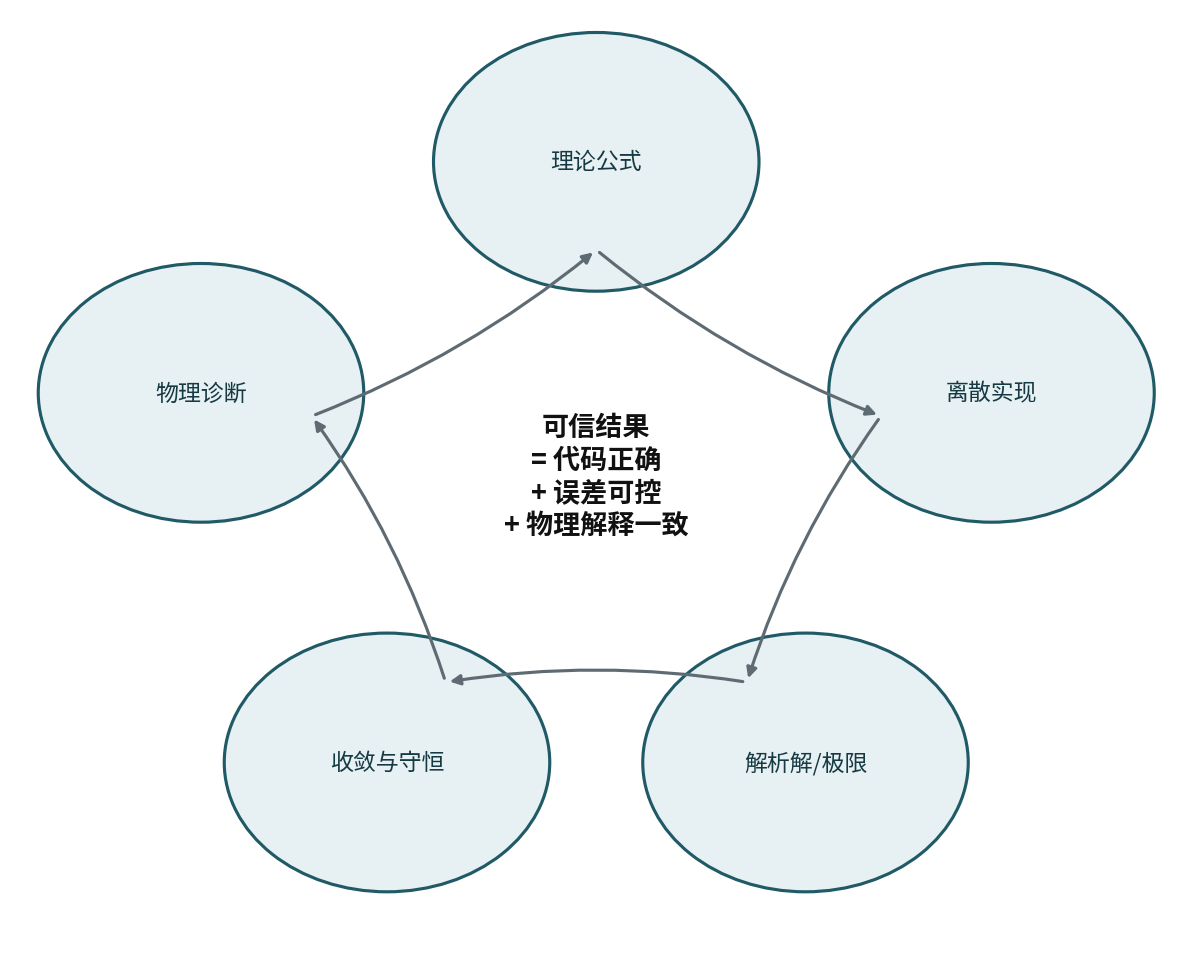
\includegraphics[width=5.98425in,height=4.78439in]{media/image3.png}

图 13-1 科学计算结果的可信验证闭环

\section{\texorpdfstring{\textbf{13.1
三套构建入口}}{13.1 三套构建入口}}\label{ux4e09ux5957ux6784ux5efaux5165ux53e3}

\textbf{表 13-1 构建系统对照}

\begin{longtable}[]{@{}llll@{}}
\toprule
\textbf{入口} & \textbf{用途} & \textbf{特点} &
\textbf{注意事项}\tabularnewline
\midrule
\endhead
Makefile & 快速构建、测试、示例 & 显式拓扑顺序，gfortran &
注释数量存在旧值\tabularnewline
fpm.toml & 标准化 Fortran 包管理 & 显式列出 41 测试与 36 示例 &
自动发现关闭，需维护清单\tabularnewline
CMakeLists.txt & 跨平台与 IDE & 对象库、静态/共享库、CTest & 构建目录与
.mod 输出需区分\tabularnewline
\bottomrule
\end{longtable}

\textbf{代码 13-1 Makefile 编译策略（Makefile:5-9）}

\begin{quote}
FC := gfortran\\
FFLAGS ?= -O2 -fPIC -Wall -Wextra -std=f2008 -ffree-line-length-none\\
AR ?= ar\\
ARFLAGS ?= rcs
\end{quote}

\section{\texorpdfstring{\textbf{13.2
测试体系}}{13.2 测试体系}}\label{ux6d4bux8bd5ux4f53ux7cfb}

项目当前有 41 个 Fortran
测试程序。测试框架是项目自实现的计数器和断言逻辑，每个测试独立编译、运行并在通过后删除临时可执行文件。其优点是依赖少，缺点是参数化、失败定位和覆盖统计能力有限。

\textbf{表 13-2 测试深度分层}

\begin{longtable}[]{@{}llll@{}}
\toprule
\textbf{测试层级} & \textbf{当前常见形式} & \textbf{能够回答的问题} &
\textbf{仍需补充}\tabularnewline
\midrule
\endhead
解析/极限 & 方势阱、无相互作用、正交性 & 公式极限是否正确 &
更多闭式解\tabularnewline
守恒/对称 & 范数、厄米性、S 幺正 & 数值结构是否保持 &
更长时间与更大参数\tabularnewline
交叉验证 & TI/TD、Python/Fortran & 独立实现是否一致 &
第三方基准\tabularnewline
收敛研究 & 当前较少 & 阶数和网格误差 & 系统性 h、dt 扫描\tabularnewline
实验验证 & 当前有限 & 模型是否描述真实系统 &
文献或实验数据\tabularnewline
\bottomrule
\end{longtable}

\begin{longtable}[]{@{}l@{}}
\toprule
\endhead
\begin{minipage}[t]{0.97\columnwidth}\raggedright
\textbf{文档残留}

README、Makefile 与实际文件数量存在版本不一致：Makefile 注释仍写 48
个核心模块、40 个测试、35 个示例；实际为 49 个核心模块、41 个测试、36
个示例。应以 fpm.toml、目录和脚本交叉核对。\strut
\end{minipage}\tabularnewline
\bottomrule
\end{longtable}

\section{\texorpdfstring{\textbf{13.3 Python
伴侣包}}{13.3 Python 伴侣包}}\label{python-ux4f34ux4fa3ux5305}

pygenmod 不是简单 f2py
绑定，而是常量、脉冲、DVR、库仑原子、HHG、转振、散射和外场散射的 Python
辅助实现。它适合教学交叉验证和绘图，但两套实现可能发生语义漂移，因此需要共享测试向量。

\section{\texorpdfstring{\textbf{13.4
可复现实验模板}}{13.4 可复现实验模板}}\label{ux53efux590dux73b0ux5b9eux9a8cux6a21ux677f}

\begin{quote}
1. 固定源码版本或文件快照，保存编译器版本和编译选项。

2. 固定随机种子、初态、网格和时间步。

3. 保存输入、单位、输出、运行命令和环境信息。

4. 对关键结果给出解析或独立实现对照。

5. 将数据、绘图脚本和最终图放在同一实验目录。
\end{quote}

\begin{longtable}[]{@{}l@{}}
\toprule
\endhead
\begin{minipage}[t]{0.97\columnwidth}\raggedright
\textbf{练习 13-1 测试升级}

\begin{quote}
1. 选择一个高级测试，增加网格和时间步收敛扫描。

2. 为 Python 与 Fortran 版本建立共享输入输出向量。

3. 修正文档中的模块、测试和示例数量，并自动检查。
\end{quote}\strut
\end{minipage}\tabularnewline
\bottomrule
\end{longtable}

\chapter{第14章 开发工具溯源、AI 协作与代码维护}\label{ux7b2c14ux7ae0-ux5f00ux53d1ux5de5ux5177ux6eafux6e90ai-ux534fux4f5cux4e0eux4ee3ux7801ux7ef4ux62a4}

用户最初的问题是：这个项目此前主要使用 OpenCode、Agy 还是 ZCode
开发。取证结果不能简单归为三者之一。能够直接确认的是 VS Code 与 Copilot
Chat Editing 在 GeneralModule 早期子项目中的使用；OpenCode、Agy 和 ZCode
都在项目目录被启动过，但没有找到当前根目录源码的专属会话记录。

\section{\texorpdfstring{\textbf{14.1
证据链}}{14.1 证据链}}\label{ux8bc1ux636eux94fe}

\textbf{表 14-1 开发工具证据强度}

\begin{longtable}[]{@{}llll@{}}
\toprule
\textbf{判断} & \textbf{直接证据} & \textbf{结论} &
\textbf{置信度}\tabularnewline
\midrule
\endhead
VS Code 用于项目 & 工作区路径、Fortran History 快照 & 确定曾使用 &
95\%\tabularnewline
Copilot 参与子项目 & github.copilot.editingSession 与 Chat Editing 记录
& 确定曾参与早期子项目 & 90\%\tabularnewline
OpenCode 启动过 & shell 历史中 opencode -c & 仅证明尝试 &
75\%\tabularnewline
Agy 启动过 & shell 历史中 agy -c & 仅证明尝试 & 75\%\tabularnewline
ZCode 启动过 & shell 历史中 zcode ./ & 仅证明尝试 & 70\%\tabularnewline
当前根目录由某一 AI 生成 & 缺少专属会话与版本历史 & 无法区分 &
≤40\%\tabularnewline
\bottomrule
\end{longtable}

\section{\texorpdfstring{\textbf{14.2
为什么不能武断归因}}{14.2 为什么不能武断归因}}\label{ux4e3aux4ec0ux4e48ux4e0dux80fdux6b66ux65adux5f52ux56e0}

\begin{itemize}
\item
  \begin{quote}
  当前根目录不是 Git 仓库，没有提交作者、提交说明和 diff 证据。
  \end{quote}
\item
  \begin{quote}
  根目录没有 .zcode、.opencode、.agy、AGENTS.md 或项目专属 VS Code
  配置。
  \end{quote}
\item
  \begin{quote}
  shell 历史没有可靠时间戳，也不能证明启动后的具体修改。
  \end{quote}
\item
  \begin{quote}
  当前源码在 2026-09-11 至 2026-09-16 集中形成，而已确认的 VS
  Code/Copilot 记录多对应更早的子项目。
  \end{quote}
\item
  \begin{quote}
  统一模板和 AI 友好文档能证明 AI 参与度高，却不能识别具体产品。
  \end{quote}
\end{itemize}

\begin{longtable}[]{@{}l@{}}
\toprule
\endhead
\begin{minipage}[t]{0.97\columnwidth}\raggedright
\textbf{最终结论}

若问题限定为``整个 GeneralModule 历史上最有证据的本地编辑环境''，答案是
VS Code，且 Copilot
确实参与过子项目。若问题限定为``当前根目录这批源码主要由
OpenCode、Agy、ZCode
中哪一个生成''，答案是现有证据不足，无法负责任地区分。\strut
\end{minipage}\tabularnewline
\bottomrule
\end{longtable}

\section{\texorpdfstring{\textbf{14.3 AI
辅助开发的正确审查方式}}{14.3 AI 辅助开发的正确审查方式}}\label{ai-ux8f85ux52a9ux5f00ux53d1ux7684ux6b63ux786eux5ba1ux67e5ux65b9ux5f0f}

\begin{quote}
1. 先要求 AI 给出假设、公式来源和算法阶数，再接受代码。

2. 把生成内容拆成可编译、可测试的小步，而不是一次性生成数百行。

3. 对每个新算法至少要求解析极限、单位测试和收敛测试。

4. 让 AI 生成测试，但由研究者决定物理上应该守恒或对称的量。

5. 使用版本控制、评审记录和会话导出，建立可追溯的生成过程。
\end{quote}

\section{\texorpdfstring{\textbf{14.4
维护建议}}{14.4 维护建议}}\label{ux7ef4ux62a4ux5efaux8bae}

\begin{itemize}
\item
  \begin{quote}
  初始化 Git 仓库并提交当前快照，避免再次失去历史归因能力。
  \end{quote}
\item
  \begin{quote}
  增加 AGENTS.md 或等价项目规则，记录 Fortran 风格、测试命令和禁止事项。
  \end{quote}
\item
  \begin{quote}
  将构建产物、编辑器状态和生成数据排除在源码之外。
  \end{quote}
\item
  \begin{quote}
  对超长模块按算法子模块拆分，但保留稳定聚合 API。
  \end{quote}
\item
  \begin{quote}
  为文档数量、文件数量和测试数量建立自动一致性检查。
  \end{quote}
\end{itemize}

\begin{longtable}[]{@{}l@{}}
\toprule
\endhead
\begin{minipage}[t]{0.97\columnwidth}\raggedright
\textbf{练习 14-1 可追溯性}

\begin{quote}
1. 为下一次 AI 协作建立提交信息模板，记录工具、提示和验证命令。

2. 设计一个脚本，从 fpm.toml 和目录自动核对测试/示例数量。

3. 列出当前项目中三个需要人工核查的注释与实现差异。
\end{quote}\strut
\end{minipage}\tabularnewline
\bottomrule
\end{longtable}

\chapter{基础理论与数值分析：从离散哈密顿量到可信量子轨迹}\label{ux57faux7840ux7406ux8bbaux4e0eux6570ux503cux5206ux6790ux4eceux79bbux6563ux54c8ux5bc6ux987fux91cfux5230ux53efux4fe1ux91cfux5b50ux8f68ux8ff9}

量子动力学计算并不是把连续薛定谔方程``翻译''为程序。它包含三次转换：先把无限维物理问题投影到有限维基底，再把连续演化近似为可重复的离散操作，最后用有限精度浮点数执行。只有每一步都有可检验的控制，我们才能把图形中的误差区分为物理效应、离散误差和代码错误。本章围绕
GeneralModule 中最常用的线性代数、FFT、DVR、Split-Operator、Lindblad
和单位转换接口，建立一套可复用的分析与排查框架。

\section{\texorpdfstring{\textbf{本章的三条判据}}{本章的三条判据}}\label{ux672cux7ae0ux7684ux4e09ux6761ux5224ux636e}

第一条是\textbf{结构判据}。投影到网格或本征基后，厄米矩阵应对称，实对称矩阵应可正交对角化，幺正演化应保内积，Lindblad
演化应保厄米、正定和迹。结构判据不依赖具体物理参数，适合先写成单元测试。例如矩阵满足
\$\textbackslash\textbar H-H\^{}T\textbackslash\textbar\$
接近机器精度、FFT
往返误差接近舍入水平、密度矩阵最小本征值不低于数值容差。若这些基础关系不成立，继续解释峰位或布居没有意义。

第二条是\textbf{收敛判据}。至少选择空间网格、时间步和基组大小中的一个参数逐级加密，在固定可观测量上估计阶数。收敛曲线应在稳定区内呈渐近斜率；若只比较两点，模型误差、边界误差与舍入平台都可能给出假象。观测量的选择也很重要：总范数对
CAP
很敏感，吸收后单调下降并非失效；布居和通道分支比可能对边界反射极敏感；近简并本征能可能收敛很快而态标签漂移。应对每类可观测量分别建立诊断量。

第三条是\textbf{物理判据}。算法必须在已知极限中恢复解析解，例如无相互作用自由粒子、谐振子能级
\$E\_v=(v+1/2)\textbackslash omega\$、退相位时布居守恒、两能级
\$\textbackslash pi\$
脉冲反转，以及单位换算往返。解析极限只验证被覆盖的物理机制，不会自动验证复杂势、多体基组或长时间动力学。它与结构、收敛判据结合，才构成对复杂结果的交叉验证。

本章的``常见错误''不是软件缺陷清单，而是思维陷阱：把守恒当作准确、把高阶当作高精度、把细网格当作无穷网格、把混合当作纠缠、把单位换算当作文字工作。真正的排查能力来自把每条理论性质改写成一个可观测量，再把可观测量接入自动测试和误差预算。

\section{\texorpdfstring{\textbf{1.
希尔伯特空间、线性算符与幺正演化}}{1. 希尔伯特空间、线性算符与幺正演化}}\label{ux5e0cux5c14ux4f2fux7279ux7a7aux95f4ux7ebfux6027ux7b97ux7b26ux4e0eux5e7aux6b63ux6f14ux5316}

\subsection{\texorpdfstring{\textbf{1.1
直觉：波函数不是``带复数的普通数组''}}{1.1 直觉：波函数不是``带复数的普通数组''}}\label{ux76f4ux89c9ux6ce2ux51fdux6570ux4e0dux662fux5e26ux590dux6570ux7684ux666eux901aux6570ux7ec4}

量子态是希尔伯特空间 \$\textbackslash mathcal H\$ 中的向量，内积记为
\$\textbackslash langle\textbackslash phi\textbar\textbackslash psi\textbackslash rangle\$。可观测性由自伴算符
\$\textbackslash hat A\$ 描述；允许的时间演化由幺正群 \$U(t)\$
描述。幺正性保证概率不因计算本身而增减，这比``下一步数值与下一步很接近''更强：它给每个时间步提供了一个结构误差计。

在有限维复空间 \$\textbackslash mathbb C\^{}N\$ 中，取厄米共轭转置

\begin{quote}
A\^{}\textbackslash dagger=(\textbackslash bar A)\^{}T.
\end{quote}

线性算符 \$A\$ 厄米当且仅当
\$A\^{}\textbackslash dagger=A\$。厄米性有三条核心后果：所有本征值为实数；不同本征值对应的本征向量正交；基底下对角矩阵为实数。第一条可由

\begin{quote}
Av=\textbackslash lambda v,\textbackslash qquad
v\^{}\textbackslash dagger Av=\textbackslash lambda
v\^{}\textbackslash dagger v
\end{quote}

及其共轭式 \$v\^{}\textbackslash dagger
Av=\textbackslash bar\textbackslash lambda v\^{}\textbackslash dagger
v\$ 得到，因 \$v\^{}\textbackslash dagger v\textgreater0\$，故
\$\textbackslash lambda=\textbackslash bar\textbackslash lambda\$。第二条来自

\begin{quote}
\textbackslash lambda\_i v\_i\^{}\textbackslash dagger
v\_j=(v\_i\^{}\textbackslash dagger
Av\_j)=(Av\_i)\^{}\textbackslash dagger v\_j
=\textbackslash bar\textbackslash lambda\_jv\_i\^{}\textbackslash dagger
v\_j.
\end{quote}

当
\$\textbackslash lambda\_i\textbackslash ne\textbackslash bar\textbackslash lambda\_j\$
时左端正数而右端为零，只能有 \$v\_i\^{}\textbackslash dagger v\_j=0\$。

\subsection{\texorpdfstring{\textbf{1.2
幺正演化的证明}}{1.2 幺正演化的证明}}\label{ux5e7aux6b63ux6f14ux5316ux7684ux8bc1ux660e}

若 \$H\^{}\textbackslash dagger=H\$，定义

\begin{quote}
U(t)=e\^{}\{-iHt\}=\textbackslash sum\_\{n=0\}\^{}\{\textbackslash infty\}\textbackslash frac\{(-iHt)\^{}n\}\{n!\}.
\end{quote}

对整个级数取共轭转置：

\begin{quote}
U(t)\^{}\textbackslash dagger=e\^{}\{iHt\}.
\end{quote}

因此 \$U\^{}\textbackslash dagger U=U U\^{}\textbackslash dagger=I\$，即
\$U\$ 幺正。由此

\begin{quote}
\textbackslash\textbar\textbackslash psi(t)\textbackslash\textbar\_2\^{}2=\textbackslash psi\^{}\textbackslash dagger(t)\textbackslash psi(t)
=\textbackslash psi\^{}\textbackslash dagger(0)U\^{}\textbackslash dagger
U\textbackslash psi(0)
=\textbackslash\textbar\textbackslash psi(0)\textbackslash\textbar\_2\^{}2.
\end{quote}

这个证明依赖两个前提：\$H\$ 厄米，以及指数运算在数学上精确实现。有限步
RK4 一般并不幺正；它可能在长时间演化中产生非物理增益。GeneralModule
的分裂算符则把厄米动能和势能分别取指数，因此在离散层面仍严格幺正。

有限维厄米矩阵还满足谱定理：存在酉矩阵 \$Q\$ 使
\$H=Q\textbackslash Lambda
Q\^{}\textbackslash dagger\$，因此酉演化可进一步写成
\$\textbackslash psi(t)=Q(e\^{}\{-i\textbackslash Lambda
t\})Q\^{}\textbackslash dagger\textbackslash psi(0)\$。这个表达式说明``幺正''与``能级为实''是同一结构的两种表述：实指数给出本征相位，酉基变换保证概率内积。它还揭示了算法选择的层次------若哈密顿量对角且谱范围适中，显式对角传播最直接；若哈密顿量稀疏或只提供矩阵---向量乘法，切比雪夫、Chebyshev
或分裂法才具有可扩展性。算法正确性应针对其逼近的演化算符讨论，不能只因输出``像波函数''就认为正确。

对两能级系统

\begin{quote}
H=\textbackslash begin\{pmatrix\}0\&a\textbackslash\textbackslash a\&0\textbackslash end\{pmatrix\},
\end{quote}

令 \$H\^{}2=a\^{}2I\$，由 \$e\^{}\{-iH\textbackslash Delta
t\}=\textbackslash cos(a\textbackslash Delta
t)I-i\textbackslash frac\{\textbackslash sin(a\textbackslash Delta
t)\}aH\$
可直接得到传播矩阵；这一闭式表达既可作为公式推导，也可作为数值实现检查。

\subsection{\texorpdfstring{\textbf{1.3 GeneralModule
源码对照}}{1.3 GeneralModule 源码对照}}\label{generalmodule-ux6e90ux7801ux5bf9ux7167}

\begin{itemize}
\item
  \begin{quote}
  `src/mod\_wavepacket\_propagator.f90`：`propagate\_split\_operator\_1d`、`propagate\_split\_operator\_2d`、`rk4\_step`、`abm4\_step`。
  \end{quote}
\item
  \begin{quote}
  `src/mod\_multistate\_coupling.f90`：`propagate\_split\_operator\_2channel`；内部用对称
  \$2\textbackslash times2\$ 矩阵指数处理两势能面耦合。
  \end{quote}
\item
  \begin{quote}
  `src/mod\_chebyshev\_propagator.f90`：`chebyshev\_propagate\_step`，通过哈密顿量谱界和矩阵---向量乘法实现大步长传播。
  \end{quote}
\item
  \begin{quote}
  `src/mod\_absorbing\_boundary.f90`：`cap\_evaluate`、`cap\_apply\_mask`。复吸收势含负虚部，是非厄米开边界，不再要求范数守恒。
  \end{quote}
\item
  \begin{quote}
  `tests/test\_propagators.f90`：检查谐振子 Split-Operator
  范数守恒；`examples/ex03\_split\_operator\_1d.f90` 展示势垒与 CAP。
  \end{quote}
\end{itemize}

\subsection{\texorpdfstring{\textbf{1.4
用不变量做最小可运行自检}}{1.4 用不变量做最小可运行自检}}\label{ux7528ux4e0dux53d8ux91cfux505aux6700ux5c0fux53efux8fd0ux884cux81eaux68c0}

下面的 Fortran 2008 片段只检查一步 Split-Operator
的厄米演化不变量。势能在本例中恒为零，因此正确结果应只是波包扩散，而范数必须保持在舍入误差量级。测试若失败，应打印每一步范数；不要用末尾归一化把失败隐藏掉。

\textbf{代码（fortran）}

\begin{quote}
use general\_module, only: dp, EYE, TWOPI, PI, \&\\
propagate\_split\_operator\_1d\\
implicit none\\
integer, parameter :: nx = 256\\
real(dp) :: dx, mass, dt, x, p0, sigma, n0, n1\\
complex(dp) :: psi(nx)\\
integer :: i\\
~\\
dx = 0.1\_dp\\
mass = 1.0\_dp\\
dt = 0.05\_dp\\
p0 = 0.7\_dp\\
sigma = 1.5\_dp\\
do i = 1, nx\\
x = -20.0\_dp + real(i-1, dp)*dx\\
psi(i) = (1.0\_dp/(PI*sigma**2)**0.25\_dp) * \&\\
exp(-0.5\_dp*((x+8.0\_dp)/sigma)**2) * \&\\
exp(EYE*p0*x)\\
end do\\
n0 = sum(abs(psi)**2)*dx\\
call propagate\_split\_operator\_1d(psi, 0.0\_dp*abs(psi), dx, mass,
dt)\\
n1 = sum(abs(psi)**2)*dx\\
print '(2ES16.8)', n0, n1
\end{quote}

无界自由粒子不在有限周期盒中严格传播，所以这个例子检验的是``程序对幺正离散公式的实现''，不是把有限盒结果当作精确自由粒子答案。若波包在一步内接近边界，正确反应是扩大盒或采用吸收/散射边界，而不是增大步长。

\subsection{\texorpdfstring{\textbf{1.5
常见错误}}{1.5 常见错误}}\label{ux5e38ux89c1ux9519ux8bef}

\begin{quote}
把``矩阵对角元为实''误当作厄米；正确检查是
\$\textbackslash\textbar A-A\^{}\textbackslash dagger\textbackslash\textbar\$。

每一步强制归一化
\$\textbackslash psi\$，借此``修复''范数漂移。若单步本应幺正则漂移是诊断量，强行归一会掩盖
FFT 符号、频率排序或吸收势错误。

对复势仍期待幺正。\$V=V-iW\$（\$W\textgreater0\$）时有
\$d\textbackslash\textbar\textbackslash psi\textbackslash\textbar\^{}2/dt=-2\textbackslash langle
W\textbackslash rangle\textbackslash\textbar\textbackslash psi\textbackslash\textbar\^{}2\$，范数下降才符合开放边界语义。

混淆可逆幺正演化与厄米时间反演演化：后者是反对称而非幺正算符。
\end{quote}

\subsection{\texorpdfstring{\textbf{1.6
小型数值例子与练习}}{1.6 小型数值例子与练习}}\label{ux5c0fux578bux6570ux503cux4f8bux5b50ux4e0eux7ec3ux4e60}

对上述二能级哈密顿量取 \$a=0.2\$、\$\textbackslash Delta
t=0.1\$，闭式传播给出 \$\textbackslash cos
0.02=0.999800\$、\$\textbackslash sin
0.02/0.2\textbackslash approx0.0999667\$。若数值积分 100 步后
\$\textbackslash\textbar\textbackslash psi\textbackslash\textbar\_2-1\textbar\textgreater10\^{}\{-6\}\$，应先检查厄米残差，再检查每一步的范数变化，而不应立刻归一化。

\textbf{练习。} 1. 用四阶 Runge--Kutta
推进同一二能级系统，扫描步长并画出
\$\textbackslash log\textbar\textbackslash\textbar\textbackslash psi(t)\textbackslash\textbar\_2-1\textbar\$。2.
解释为什么切比雪夫法的截断误差可与谱宽 \$\textbackslash Delta
E\textbackslash Delta t\$ 联系起来。3. 对含 CAP
的轨迹，什么量应守恒，什么量应单调减少？

\section{\texorpdfstring{\textbf{2.
傅里叶变换、离散谱与采样定理}}{2. 傅里叶变换、离散谱与采样定理}}\label{ux5085ux91ccux53f6ux53d8ux6362ux79bbux6563ux8c31ux4e0eux91c7ux6837ux5b9aux7406}

\subsection{\texorpdfstring{\textbf{2.1
直觉：改变基底以暴露对角结构}}{2.1 直觉：改变基底以暴露对角结构}}\label{ux76f4ux89c9ux6539ux53d8ux57faux5e95ux4ee5ux66b4ux9732ux5bf9ux89d2ux7ed3ux6784}

薛定谔方程中，动能算符在坐标表象写为微分算符，在动量表象却写为乘法算符
\$p\^{}2/(2m)\$。傅里叶变换不是数值加速技巧，而是选择最容易执行的物理基底。采用约定

\begin{quote}
\textbackslash tilde\textbackslash psi(k)=\textbackslash frac1\{\textbackslash sqrt\{2\textbackslash pi\}\}\textbackslash int\_\{-\textbackslash infty\}\^{}\{\textbackslash infty\}\textbackslash psi(x)e\^{}\{-ikx\}\textbackslash,dx.
\end{quote}

对 \$N\$ 个等距样本，GeneralModule 实现未归一化正变换和带 \$1/N\$
的逆变换：

\begin{quote}
\textbackslash tilde\textbackslash psi\_j=\textbackslash sum\_\{n=0\}\^{}\{N-1\}\textbackslash psi\_n
e\^{}\{-2\textbackslash pi i jn/N\}, \textbackslash qquad
\textbackslash psi\_n=\textbackslash frac1N\textbackslash sum\_\{j=0\}\^{}\{N-1\}\textbackslash tilde\textbackslash psi\_j
e\^{}\{2\textbackslash pi i jn/N\}.
\end{quote}

正、逆公式逐项相乘并对 \$j\$ 求和，由复指数正交关系

\begin{quote}
\textbackslash sum\_\{j=0\}\^{}\{N-1\}e\^{}\{2\textbackslash pi
i(j-l)n/N\}=N\textbackslash delta\_\{jl\}
\end{quote}

立即得到 \$\textbackslash psi\_n\$，即逆变换正确。

\subsection{\texorpdfstring{\textbf{2.2
离散频率、周期性与采样定理}}{2.2 离散频率、周期性与采样定理}}\label{ux79bbux6563ux9891ux7387ux5468ux671fux6027ux4e0eux91c7ux6837ux5b9aux7406}

DFT 默认样本位于周期为 \$L=N\textbackslash Delta x\$
的圆周上，频率间隔为 \$\textbackslash Delta
k=2\textbackslash pi/L\$。若函数严格带限于
\${[}-k\_\{\textbackslash max\},k\_\{\textbackslash max\}{]}\$，为避免周期延拓在端点拼接造成频谱混叠，应满足

\begin{quote}
k\_\{\textbackslash max\}\textless\textbackslash frac\{\textbackslash pi\}\{\textbackslash Delta
x\},
\end{quote}

并取足够点数覆盖记录长度。等价的 Nyquist 条件是 \$\textbackslash Delta
x\textless\textbackslash pi/k\_\{\textbackslash max\}\$。DFT
可无歧义表示的频率在 \${[}-\textbackslash pi/\textbackslash Delta
x,\textbackslash pi/\textbackslash Delta x)\$
中；\$p\_\{\textbackslash max\}=\textbackslash pi/\textbackslash Delta
x\$ 是网格能分辨的最高动量。

有限时间窗等价于对信号乘矩形窗，其频谱与理想连续谱卷积。窗越短，频率分辨率越差：若时间跨度
\$T\$，不含窗函数展宽的频率分辨率约为
\$2\textbackslash pi/T\$。因此``高时间采样率''和``高谱分辨率''不是同一要求：前者要求
\$\textbackslash Delta t\$ 足够小，后者要求记录足够长。

还需区分``离散频率坐标''与``物理频率''。在给定 \$\textbackslash Delta
t\$ 下，DFT 的频率间隔
\$\textbackslash Delta\textbackslash omega=2\textbackslash pi/(N\textbackslash Delta
t)\$；改变窗口长度会改变网格间隔，峰的位置通常近似不变，但可表示的带宽发生变化。相反，改变
\$\textbackslash Delta t\$ 而保持总时长 \$N\textbackslash Delta t\$
不变，会细化频率网格，却不改善由总时长决定的分辨极限。实验上常见``过采样后谱峰仍不移动''的现象，原因正是物理分辨极限由时间窗而非绘图点数决定。

\subsection{\texorpdfstring{\textbf{2.3 Parseval
关系与动量算符}}{2.3 Parseval 关系与动量算符}}\label{parseval-ux5173ux7cfbux4e0eux52a8ux91cfux7b97ux7b26}

离散 Parseval 定理给出

\begin{quote}
\textbackslash Delta
x\textbackslash sum\_\{n=0\}\^{}\{N-1\}\textbar\textbackslash psi\_n\textbar\^{}2
=\textbackslash frac1N\textbackslash sum\_\{j=0\}\^{}\{N-1\}\textbar\textbackslash tilde\textbackslash psi\_j\textbar\^{}2.
\end{quote}

由 Fourier 表象中的微分关系
\$\textbackslash partial\_x\textbackslash psi\textbackslash leftrightarrow
ik\textbackslash tilde\textbackslash psi\$，动量平均值为

\begin{quote}
\textbackslash langle
p\textbackslash rangle=\textbackslash frac\{(1/N)\textbackslash sum\_j
k\_j\textbar\textbackslash tilde\textbackslash psi\_j\textbar\^{}2\}
\{\textbackslash sum\_j\textbar\textbackslash tilde\textbackslash psi\_j\textbar\^{}2\}.
\end{quote}

源码中的索引先把正频率放在数组前半部，再把负频率映射到数组后半部；这避免了盲目把数组后半部当成正的大动量，是动量量算正确的前提。

\subsection{\texorpdfstring{\textbf{2.4 GeneralModule
源码对照}}{2.4 GeneralModule 源码对照}}\label{generalmodule-ux6e90ux7801ux5bf9ux7167-1}

\begin{itemize}
\item
  \begin{quote}
  `src/mod\_linear\_algebra.f90`：`fft\_1d(data\_vec,
  isign)`，`isign=-1` 为正变换、`+1` 为逆变换；`fft\_2d`
  沿两维依次调用一维 FFT。
  \end{quote}
\item
  \begin{quote}
  非 \$2\$ 的幂长度会自动回退到 \$O(N\^{}2)\$
  DFT。物理上正确，但大网格可能突然变慢。
  \end{quote}
\item
  \begin{quote}
  `src/mod\_wavepacket\_propagator.f90`：以 \$p\_j\^{}2/(2m)\$
  构造动量相位，是 Split-Operator 的核心。
  \end{quote}
\item
  \begin{quote}
  `tests/test\_propagators.f90` 用范数守恒间接检验正逆变换配对。
  \end{quote}
\end{itemize}

可用以下往返变换同时检查归一化约定、数组长度与舍入稳定性：

\textbf{代码（fortran）}

\begin{quote}
use general\_module, only: dp, EYE, TWOPI, fft\_1d\\
implicit none\\
integer, parameter :: n = 1024\\
real(dp) :: dx, k0, sigma, roundtrip\_error\\
complex(dp) :: x(n), original(n)\\
integer :: j\\
~\\
dx = 0.05\_dp\\
k0 = 1.3\_dp\\
sigma = 2.0\_dp\\
do j = 1, n\\
x(j) = exp(-0.5\_dp*((real(j-1,dp)-n/2)*dx/sigma)**2) * \&\\
exp(EYE*k0*real(j-1,dp)*dx)\\
end do\\
original = x\\
call fft\_1d(x, -1)\\
call fft\_1d(x, +1)\\
roundtrip\_error = maxval(abs(x-original))\\
print '(ES16.8)', roundtrip\_error
\end{quote}

误差随 \$N\$ 的增长应大致满足
\$O(\textbackslash varepsilon\textbackslash log\_2N)\$，而不是
\$O(N)\$。若结果随长度呈平方增长，应检查是否触发了非 \$2\$
的幂回退以及测试数据是否在回退路径上出现异常。

\subsection{\texorpdfstring{\textbf{2.5
常见错误}}{2.5 常见错误}}\label{ux5e38ux89c1ux9519ux8bef-1}

\begin{quote}
把逆变换也按正变换归一化，导致振幅相差 \$N\$。

不检查 `isign`，或二维变换中两维次序不一致。

动量网格的负频率分支未映射。能量因 \$p\^{}2\$
对正负号不敏感，平均动量却会立刻暴露错误。

高动量波包越过 \$p\_\{\textbackslash max\}\$
后在周期边界卷回，与低能波包重叠，形成人为混叠。

把 FFT 浮点舍入误认为物理噪声；规范形为
\$\textbackslash varepsilon\textbackslash log\_2N\$ 级的快速增长。
\end{quote}

\subsection{\texorpdfstring{\textbf{2.6
小型数值例子}}{2.6 小型数值例子}}\label{ux5c0fux578bux6570ux503cux4f8bux5b50}

令复指数 \$f\_n=e\^{}\{i0.6\textbackslash pi n\textbackslash Delta
t\}\$、\$N=8\$。Nyquist 频率为 \$\textbackslash pi/\textbackslash Delta
t\$，但 DFT 只能表示离散频率
\$-4/8,-3/8,\textbackslash ldots,3/8\$。由于对整数 \$n\$ 有
\$e\^{}\{i0.6\textbackslash pi n\}=e\^{}\{-i0.4\textbackslash pi
n\}\$，这些样本完全等于 \$e\^{}\{-i0.4\textbackslash pi
n\textbackslash Delta t\}\$，正频率被别名为负的离散频率
\$0.375\textbackslash pi/\textbackslash Delta
t\$。若错误地只取实部并忽略正负号，还会得到
\$\textbackslash cos(0.6\textbackslash pi n\textbackslash Delta
t)=-\textbackslash cos(0.4\textbackslash pi n\textbackslash Delta
t)\$，进一步改变结果。频谱图看似``干净''，物理结论却已错误。加密 \$N\$
不会自动消除这种基带采样别名；必须先降低 \$\textbackslash Delta t\$
或预滤波。这个例子还说明：混叠不是额外出现一个``错误高线''，而是高频分量可以完全伪装成某个合法低频分量。

\textbf{练习。} 1. 验证 `fft\_1d(fft\_1d(x,-1),1)` 与原向量之差随 \$N\$
的变化。2. 构造带限高斯波包，给出至少三个网格加密方案并比较
\$\textbackslash langle p\^{}2\textbackslash rangle\$。3.
对高斯时间窗，验证时间跨度加倍后谱峰宽度约减半。4.
对含零均值噪声的信号，比较矩形窗与 Gaussian 窗的主瓣宽度和旁瓣泄漏。

\section{\texorpdfstring{\textbf{3.
本征问题、矩阵范数、条件数与误差传播}}{3. 本征问题、矩阵范数、条件数与误差传播}}\label{ux672cux5f81ux95eeux9898ux77e9ux9635ux8303ux6570ux6761ux4ef6ux6570ux4e0eux8befux5deeux4f20ux64ad}

\subsection{\texorpdfstring{\textbf{3.1
本征问题的正确性判据}}{3.1 本征问题的正确性判据}}\label{ux672cux5f81ux95eeux9898ux7684ux6b63ux786eux6027ux5224ux636e}

离散哈密顿量满足

\begin{quote}
Hv\_\textbackslash alpha=E\_\textbackslash alpha
v\_\textbackslash alpha.
\end{quote}

本征向量只有方向意义：\$v\_\textbackslash alpha\$ 与
\$e\^{}\{i\textbackslash theta\_\textbackslash alpha\}v\_\textbackslash alpha\$
等价。近简并态的混合基也具有等价性，因此不要把单个本征向量或其符号当作绝对物理量。实对称矩阵满足谱定理

\begin{quote}
H=Q\textbackslash Lambda Q\^{}T,\textbackslash qquad
\textbackslash Lambda=\textbackslash operatorname\{diag\}(E\_\textbackslash alpha).
\end{quote}

GeneralModule 的 `diag\_symmetric\_matrix` 先以 Householder
反射作正交相似变换

\begin{quote}
T=Q\^{}THQ
\end{quote}

把矩阵压缩为三对角形，再以带位移的 QL 迭代求谱并累积 \$Q\$；最终 `d(i)`
是升序本征值，`z(:,i)` 才是对应本征向量。

\subsection{\texorpdfstring{\textbf{3.2 Rayleigh
商、能量与残差}}{3.2 Rayleigh 商、能量与残差}}\label{rayleigh-ux5546ux80fdux91cfux4e0eux6b8bux5dee}

Rayleigh 商

\begin{quote}
R(v)=\textbackslash frac\{v\^{}THv\}\{v\^{}Tv\}
\end{quote}

在单位本征向量上给出能量。数值上应同时报告能量和归一化残差

\begin{quote}
\textbackslash varepsilon\_\textbackslash alpha=\textbackslash\textbar Hv\_\textbackslash alpha-E\_\textbackslash alpha
v\_\textbackslash alpha\textbackslash\textbar\_2.
\end{quote}

对精确对称矩阵，Weyl 不等式给出

\begin{quote}
\textbar\textbackslash widetilde
E\_\textbackslash alpha-E\_\textbackslash alpha\textbar\textbackslash le
\textbackslash\textbar H-\textbackslash widetilde
H\textbackslash\textbar\_2.
\end{quote}

因此，如果势能插值误差使 \$\textbackslash\textbar\textbackslash Delta
V\textbackslash\textbar\_2\textbackslash le 10\^{}\{-6\}\$
Hartree，则任一本征值的移动不超过该界；但如果近简并，本征向量会强烈旋转，能级曲线稳定并不代表态的物理标签稳定。

对简并空间
\$P\_\textbackslash alpha=\textbackslash sum\_\{\textbackslash beta\textbackslash in\textbackslash alpha\}v\_\textbackslash beta
v\_\textbackslash beta\^{}T\$，扰动后的投影变化在基向量选择下不变，却可用
\$\textbackslash\textbar P\_\textbackslash alpha\textbackslash widetilde
P\_\textbackslash alpha-\textbackslash widetilde P\_\textbackslash alpha
P\_\textbackslash alpha\textbackslash\textbar\_2\$ 衡量。若能隙
\$\textbackslash Delta=\textbar E\_\{\textbackslash alpha+1\}-E\_\textbackslash alpha\textbar\$
远大于扰动 \$\textbackslash\textbar{} \textbackslash Delta
H\textbackslash\textbar\_2\$，本征向量基本稳定；若二者同量级，只有简并子空间整体可辨。对非厄米或非正规矩阵，即便本征值都``看起来正常''，也可能出现瞬时放大，所以量子计算应优先使用厄米自伴表示和正交归一化。

\subsection{\texorpdfstring{\textbf{3.3
范数与条件数}}{3.3 范数与条件数}}\label{ux8303ux6570ux4e0eux6761ux4ef6ux6570}

常用矩阵范数为

\begin{quote}
\textbackslash\textbar A\textbackslash\textbar\_1=\textbackslash max\_j\textbackslash sum\_i\textbar a\_\{ij\}\textbar,\textbackslash quad
\textbackslash\textbar A\textbackslash\textbar\_\textbackslash infty=\textbackslash max\_i\textbackslash sum\_j\textbar a\_\{ij\}\textbar,\textbackslash quad
\textbackslash\textbar A\textbackslash\textbar\_2=\textbackslash sigma\_\{\textbackslash max\}(A),
\end{quote}

Frobenius 范数
\$\textbackslash\textbar A\textbackslash\textbar\_F=(\textbackslash sum\_\{ij\}\textbar a\_\{ij\}\textbar\^{}2)\^{}\{1/2\}\$
便于衡量全部元素误差。条件数

\begin{quote}
\textbackslash kappa\_2(A)=\textbackslash\textbar A\textbackslash\textbar\_2\textbackslash\textbar A\^{}\{-1\}\textbackslash\textbar\_2
=\textbackslash frac\{\textbackslash sigma\_\{\textbackslash max\}\}\{\textbackslash sigma\_\{\textbackslash min\}\}
\end{quote}

度量相对输入误差向相对输出误差的最大放大。Gauss--Jordan
求逆中，一个主元舍入误差在最坏情况下可产生约
\$\textbackslash kappa(A)u\$ 的相对误差，其中 \$u\$
为机器精度。若只做矩阵---向量乘法，通常
\$\textbackslash\textbar A\textbackslash delta
x\textbackslash\textbar/(\textbackslash\textbar A\textbackslash\textbar\textbackslash\textbar x\textbackslash\textbar)\$
更能反映实际前向误差，不应机械地总用条件数。

对近奇异矩阵

\begin{quote}
A=\textbackslash begin\{pmatrix\}1\&1\textbackslash\textbackslash1\&1+10\^{}\{-8\}\textbackslash end\{pmatrix\},
\end{quote}

本征值约为 \$2.00000001\$ 与 \$10\^{}\{-8\}\$，故
\$\textbackslash kappa\_2(A)\textbackslash approx2.0\textbackslash times10\^{}8\$。即便每个矩阵元只扰动约
\$10\^{}\{-16\}\$，逆矩阵某些分量也可出现 \$10\^{}\{-8\}\$
量级相对误差。若目标能级精度是 \$10\^{}\{-10\}\$
Hartree，这个矩阵显然不适合通过通用求逆来解耦合线性方程。

\subsection{\texorpdfstring{\textbf{3.4 GeneralModule
源码对照}}{3.4 GeneralModule 源码对照}}\label{generalmodule-ux6e90ux7801ux5bf9ux7167-2}

\begin{itemize}
\item
  \begin{quote}
  `src/mod\_linear\_algebra.f90`：`diag\_symmetric\_matrix(n,a\_in,d,z,stat)`、`inv\_real\_matrix`、`inv\_complex\_matrix`。
  \end{quote}
\item
  \begin{quote}
  逆矩阵例程使用全主元 Gauss--Jordan；主元小于固定阈值 \$10\^{}\{-30\}\$
  时返回 `stat=-1`。
  \end{quote}
\item
  \begin{quote}
  `src/mod\_dvr\_grid.f90`：`fgh\_solve\_bound\_states` 构造 \$H=T+V\$
  并调用实对称本征求解器。
  \end{quote}
\item
  \begin{quote}
  `tests/test\_dvr\_grid.f90` 验证 Sinc-DVR
  动能矩阵对称性及谐振子能级；`examples/ex01\_fgh\_diatomic\_bound\_states.f90`
  与 Morse 解析能级比较。
  \end{quote}
\end{itemize}

可把``求解成功''提升为``解可验证''：除检查返回码，还应检查本征残差、Rayleigh
商和正交性。以下片段对任意实对称 \$2\textbackslash times2\$
矩阵都能运行。

\textbf{代码（fortran）}

\begin{quote}
use general\_module, only: dp, diag\_symmetric\_matrix\\
implicit none\\
real(dp) :: a(2,2), e(2), z(2,2), hz(2,2), zz(2,2)\\
real(dp) :: residual, orth\_error, rayleigh\\
integer :: stat, i, j\\
~\\
a = reshape({[}1.0\_dp, 0.2\_dp, 0.2\_dp, 0.8\_dp{]}, {[}2,2{]})\\
call diag\_symmetric\_matrix(2, a, e, z, stat)\\
hz = matmul(a, z)\\
do j = 1, 2\\
do i = 1, 2\\
hz(i,j) = hz(i,j) - e(j)*z(i,j)\\
end do\\
end do\\
residual = maxval(abs(hz))\\
zz = matmul(transpose(z), z)\\
orth\_error = maxval(abs(zz - {[}1.0\_dp,0.0\_dp,0.0\_dp,1.0\_dp{]}))\\
rayleigh = dot\_product(z(:,1), matmul(a, z(:,1))) / \&\\
dot\_product(z(:,1), z(:,1))\\
print '(I3, 3ES16.8)', stat, residual, orth\_error, rayleigh
\end{quote}

对大矩阵，逐个构造完整 \$H\textbackslash Lambda\$ 会浪费内存，可按列计算
\$\textbackslash\textbar(Hz)\_:,i-E\_i
z\_:,i\textbackslash\textbar\_2\$，并只求范数而不复制矩阵。验证成本应低于求解成本，但不能为省一次检查而完全省略验证。

\subsection{\texorpdfstring{\textbf{3.5
常见错误}}{3.5 常见错误}}\label{ux5e38ux89c1ux9519ux8bef-2}

\begin{quote}
忽略 `stat`，在未收敛时继续解释本征态。

把 `z(i,:)` 误认为第 \$i\$ 个本征态；本征态在第 \$i\$ 列。

只对输入矩阵作一次``上三角化''，却把未累积的正交矩阵当作结果；Householder
约化和特征向量累积缺一不可。

用绝对阈值 \$10\^{}\{-30\}\$
判断所有矩阵的奇异性，未考虑行列缩放。对能量量级相差 \$10\^{}\{12\}\$
的耦合方程，同一阈值含义不同。

近简并时比较``本征向量逐点差''；必须比较投影矩阵或谱投影。交换简并基不构成物理错误。
\end{quote}

\textbf{练习。} 1. 构造带随机小扰动的 \$10\textbackslash times10\$
对称矩阵，检验
\$\textbackslash\textbar HQ-Q\textbackslash Lambda\textbackslash\textbar\$。2.
将上例矩阵整体缩放 \$10\^{}\{100\}\$ 和
\$10\^{}\{-100\}\$，讨论固定主元阈值的局限。3.
对近简并二能级系统，画出能量和本征态投影随扰动的变化。

\section{\texorpdfstring{\textbf{4. ODE/PDE 数值方法、稳定性与 Lax
等价性思想}}{4. ODE/PDE 数值方法、稳定性与 Lax 等价性思想}}\label{odepde-ux6570ux503cux65b9ux6cd5ux7a33ux5b9aux6027ux4e0e-lax-ux7b49ux4ef7ux6027ux601dux60f3}

\subsection{\texorpdfstring{\textbf{4.1
从连续方程到离散格式}}{4.1 从连续方程到离散格式}}\label{ux4eceux8fdeux7eedux65b9ux7a0bux5230ux79bbux6563ux683cux5f0f}

连续薛定谔方程可视为线性 ODE 族

\begin{quote}
i\textbackslash hbar\textbackslash frac\{\textbackslash partial\textbackslash psi\}\{\textbackslash partial
t\}=H(t)\textbackslash psi.
\end{quote}

数值法只有在以下三项同时成立时才可信：局部截断误差随步长消失；数值稳定性给出不随网格加密而爆发的误差界；一致的离散问题在细网格极限下逼近原问题。Lax--Richtmyer
等价性定理的常用表述是：在固定计算区间上，\textbf{一致性加稳定性推出收敛}。这里的``固定''很重要；若把终止时间随网格加密而增大，反问题会引入额外稳定性限制。

PDE
离散还须指定边界。Dirichlet、Neumann、吸收边界和周期边界不是可互换的数值细节，而是不同物理模型。周期
FFT 边界要求波包在网格首尾及多圈之后都不接触；CAP
则允许范数单调流出计算域。

\subsection{\texorpdfstring{\textbf{4.2 Strang
分裂为何正确}}{4.2 Strang 分裂为何正确}}\label{strang-ux5206ux88c2ux4e3aux4f55ux6b63ux786e}

令 \$H=T+V\$。Strang 一步为

\begin{quote}
S(\textbackslash Delta t)=e\^{}\{-iT\textbackslash Delta
t/2\}e\^{}\{-iV\textbackslash Delta t\} e\^{}\{-iT\textbackslash Delta
t/2\}.
\end{quote}

将 BCH 公式展开，\$T\$ 与 \$V\$ 的对易子只在 \$\textbackslash Delta
t\^{}3\$ 项首次出现，因此单步局部误差为 \$O(\textbackslash Delta
t\^{}3)\$；经过 \$1/\textbackslash Delta t\$ 步累积后，全局误差为二阶：

\begin{quote}
S(\textbackslash Delta t)\^{}\{n\}=e\^{}\{-iH t\}+O(\textbackslash Delta
t\^{}2).
\end{quote}

每一步都是两个幺正矩阵的乘积，所以每一步以及整个离散步列都幺正。这个性质强于许多四阶
ODE 格式：对长时间量子相干，分裂法的结构误差更可控。若用一般权重
\$e\^{}\{-iaT\textbackslash Delta t\}e\^{}\{-ibV\textbackslash Delta
t\}\$，在 \$a+b=1\$ 时通常为二阶，对称选择才给出 Strang
的时间可逆性。对多部分
\$H=\textbackslash sum\_jH\_j\$，各部分应先组合成互相对易的群，例如动量方向、相互作用方向和外部势能；把明显不对易的耦合随意拆开会产生不可控的分裂误差。旋转波近似也应视为对易子被假设很小，而不是无条件精确。

Lax
思想还提醒我们：稳定性依赖问题类型。对初值问题，稳定性通常指误差在固定时间区间不爆炸；对长时间量子相干，所需的往往更强------离散演化保持幺正、能量位于允许范围。满足其中一个并不自动满足另一个。数值上应同时报告稳定性和物理不变量，二者缺一不可。

\subsection{\texorpdfstring{\textbf{4.3
显式格式的放大因子}}{4.3 显式格式的放大因子}}\label{ux663eux5f0fux683cux5f0fux7684ux653eux5927ux56e0ux5b50}

对简单模型 \$y'=iEy\$，显式 Euler 得

\begin{quote}
y\_\{n+1\}=(1+iE\textbackslash Delta t)y\_n,\textbackslash qquad
\textbar1+iE\textbackslash Delta
t\textbar=\textbackslash sqrt\{1+(E\textbackslash Delta
t)\^{}2\}\textgreater1,
\end{quote}

每步都引入非物理增益，和算法的``形式阶数''是两回事。RK4
对许多线性常系数方程局部精度高，但一般不保幺正。其局部稳定域可由放大因子多项式刻画，边界大致在虚轴
\$\textbackslash pm
2\textbackslash sqrt2\$；这不等于对所有非自治量子问题都稳定。

对显式扩散格式，最可靠的检查是 von Neumann 稳定性分析。设误差模态为
\$\textbackslash varepsilon\_j\^{}n=e\^{}\{ikx\_j\}\textbackslash hat\textbackslash varepsilon\^{}n\$，离散符号给出
\$\textbar\textbackslash lambda(\textbackslash Delta
t,k)\textbar\textbackslash le1\$ 的条件。例如一维显式热方程

\begin{quote}
u\_j\^{}\{n+1\}=u\_j\^{}n+\textbackslash alpha\textbackslash Delta
t(u\_\{j+1\}\^{}n-2u\_j\^{}n+u\_\{j-1\}\^{}n), \textbackslash qquad
\textbackslash alpha=\textbackslash frac\{\textbackslash Delta
t\}\{\textbackslash Delta x\^{}2\},
\end{quote}

其最坏模态 \$k\textbackslash Delta x=\textbackslash pi\$ 给出放大因子
\$1-4\textbackslash alpha\$，故稳定条件为
\$\textbackslash alpha\textbackslash le1/2\$。这是由符号分析得到的充分判据，不是经验调参。

\subsection{\texorpdfstring{\textbf{4.4
步长、空间网格与吸收边界}}{4.4 步长、空间网格与吸收边界}}\label{ux6b65ux957fux7a7aux95f4ux7f51ux683cux4e0eux5438ux6536ux8fb9ux754c}

步长小并不保证空间误差小，反之亦然。高能自由传播要求
\$p\_\{\textbackslash max\}=\textbackslash pi/\textbackslash Delta x\$
高于波包所含动量；强场问题还要让激光载频、脉冲包络和高次谐波都能在网格与时间步上分辨。对
Split-Operator，动能相位本身是精确酉的，没有 Euler 式增长，但
\$\textbackslash Delta E\_\{\textbackslash max\}\textbackslash Delta t\$
过大仍会产生相位欠采样和能量谱污染。

\subsection{\texorpdfstring{\textbf{4.5 GeneralModule
源码对照}}{4.5 GeneralModule 源码对照}}\label{generalmodule-ux6e90ux7801ux5bf9ux7167-3}

\begin{itemize}
\item
  \begin{quote}
  `src/mod\_wavepacket\_propagator.f90`：`propagate\_split\_operator\_1d/2d`
  实现二阶对称分裂；`rk4\_step` 与 `abm4\_step` 是通用 ODE 步进接口。
  \end{quote}
\item
  \begin{quote}
  `src/mod\_open\_quantum.f90`：`rk4\_lindblad\_step` 推进 Lindblad
  方程，并在每步后厄米化与归一化。
  \end{quote}
\item
  \begin{quote}
  `src/mod\_absorbing\_boundary.f90`：`cap\_evaluate` 与
  `cap\_apply\_mask`；`calculate\_probability\_flux`
  用二阶中心差分计算通量。
  \end{quote}
\item
  \begin{quote}
  `examples/ex06\_two\_state\_nonadiabatic.f90`
  是多势能面动力学；`tests/test\_propagators.f90` 检查 Split-Operator 与
  Bloch 矢量范数。
  \end{quote}
\end{itemize}

稳定性与收敛性必须分别测量。下面的研究循环对同一总时间使用
\$N\$、\$2N\$、\$4N\$
个时间步，并同时输出范数和步数拟合斜率。若范数先变差而能量误差看似稳定，不应立即宣布二阶收敛，因为那可能只是守恒量的误差被投影补偿。

\textbf{代码（fortran）}

\begin{quote}
program step\_refinement\\
use general\_module, only: dp, PI, TWOPI, fft\_1d, \&\\
propagate\_split\_operator\_1d\\
implicit none\\
integer, parameter :: nx = 512\\
integer :: nsteps, nrun, step, i, j\\
real(dp) :: xmin, xmax, dx, dt, t\_end, norm, e\_ref\\
real(dp), parameter :: sigma = 1.0\_dp\\
real(dp) :: x(nx), v(nx), energy\_error(3)\\
complex(dp) :: psi(nx), psi0(nx)\\
~\\
xmin = -12.0\_dp; xmax = 12.0\_dp\\
dx = (xmax-xmin)/real(nx,dp)\\
t\_end = 5.0\_dp\\
do i = 1, nx\\
x(i) = xmin + real(i-1,dp)*dx\\
v(i) = 0.5\_dp*x(i)**2\\
psi0(i) = (1.0\_dp/(PI*sigma**2)**0.25\_dp) * \&\\
exp(-0.5\_dp*(x(i)/sigma)**2)\\
end do\\
e\_ref = energy(psi0, v, dx)\\
do nrun = 1, 3\\
nsteps = 100*2**(nrun-1)\\
dt = t\_end/real(nsteps,dp)\\
psi = psi0\\
do step = 1, nsteps\\
call propagate\_split\_operator\_1d(psi, v, dx, 1.0\_dp, dt)\\
end do\\
norm = sum(abs(psi)**2)*dx\\
energy\_error(nrun) = abs(energy(psi,v,dx) - e\_ref)\\
print '(I6,2ES14.6)', nsteps, abs(norm-1.0\_dp), energy\_error(nrun)\\
end do\\
contains\\
function energy(p, vgrid, hgrid) result(e)\\
complex(dp), intent(in) :: p(:)\\
real(dp), intent(in) :: vgrid(:), hgrid\\
real(dp) :: e, pmean\\
complex(dp) :: work(nx)\\
integer :: k\\
work = p\\
call fft\_1d(work, -1)\\
pmean = 0.0\_dp\\
do k = 1, nx\\
if (k \textless= nx/2) then\\
pmean = pmean + real(k-1,dp)*(2.0\_dp*TWOPI/ \&\\
(real(nx,dp)*hgrid))*abs(work(k))**2\\
else\\
pmean = pmean + real(k-1-nx,dp)*(2.0\_dp*TWOPI/ \&\\
(real(nx,dp)*hgrid))*abs(work(k))**2\\
end if\\
end do\\
e = 0.5\_dp*pmean/real(nx,dp) + \&\\
sum(conjg(p)*vgrid*p)*hgrid\\
end function energy\\
end program step\_refinement
\end{quote}

实际工程中可用更简洁的带符号动量索引重构能量循环；这里保留显式形式，是为了让读者看清负频率分支。关键是固定网格只改步长，再固定步长只改网格，两条研究线不能混在一起，否则拟合出的阶数没有解释意义。

\subsection{\texorpdfstring{\textbf{4.6
常见错误}}{4.6 常见错误}}\label{ux5e38ux89c1ux9519ux8bef-3}

\begin{quote}
混淆一致性与稳定性：公式截断误差 \$O(\textbackslash Delta t)\$
正确，不代表可取任意大步长。

给定非 \$2\$ 的幂 FFT 长度后只关注正确性，忽视自动回退到 \$O(N\^{}2)\$
的性能突变。

波包已到边界才加大 CAP；吸收起点应早于强相互作用区，且末端斜率平缓。

ABM 历史导数错位，或启动多步法时没有足够初值。

用总范数下降作为唯一质量指标；开启 CAP
后还应同时监测内部范数、吸收通量与反射回波。
\end{quote}

\subsection{\texorpdfstring{\textbf{4.7
小型数值例子}}{4.7 小型数值例子}}\label{ux5c0fux578bux6570ux503cux4f8bux5b50-1}

对谐振子 \$H=p\^{}2/2+x\^{}2/2\$，取 \$\textbackslash omega=1\$。显式
Euler 用 \$\textbackslash Delta t=0.1\$ 推进一步，Euler 模态放大因子约为
\$1.00499\$，100 步后放大约 \$1.65\$；Strang 单步每种模态的模仍为
1。这说明``步长看起来足够小''和``物理不变量被破坏''可能同时出现。将
\$\textbackslash Delta t\$ 减半，Strang 全局误差应按约 \$4\$ 倍下降。

\textbf{练习。} 1. 对含时谐振子同时扫描 \$\textbackslash Delta x\$ 与
\$\textbackslash Delta t\$，分离空间和时间误差。2. 给高斯波包加
CAP，分别比较 \$\textbackslash sin\^{}2\$ 与三次多项式型反射。3.
推导显式热方程的一维 CFL 条件，并推广到 \$D\$ 维。

\section{\texorpdfstring{\textbf{5.
量子态、密度矩阵、纠缠、纯度与熵}}{5. 量子态、密度矩阵、纠缠、纯度与熵}}\label{ux91cfux5b50ux6001ux5bc6ux5ea6ux77e9ux9635ux7ea0ux7f20ux7eafux5ea6ux4e0eux71b5}

\subsection{\texorpdfstring{\textbf{5.1
纯态、混合态与约化密度矩阵}}{5.1 纯态、混合态与约化密度矩阵}}\label{ux7eafux6001ux6df7ux5408ux6001ux4e0eux7ea6ux5316ux5bc6ux5ea6ux77e9ux9635}

纯态 \$\textbar\textbackslash psi\textbackslash rangle\$
可由波函数表示，混合态则由密度矩阵

\begin{quote}
\textbackslash rho=\textbackslash sum\_\textbackslash mu
p\_\textbackslash mu\textbar\textbackslash psi\_\textbackslash mu\textbackslash rangle\textbackslash langle\textbackslash psi\_\textbackslash mu\textbar{}
\end{quote}

表示。物理条件是
\$\textbackslash rho\^{}\textbackslash dagger=\textbackslash rho\$、\$\textbackslash rho\textbackslash succeq0\$、\$\textbackslash operatorname\{Tr\}\textbackslash rho=1\$。单一波函数
\$\textbackslash psi\$ 对应
\$\textbackslash rho=\textbar\textbackslash psi\textbackslash rangle\textbackslash langle\textbackslash psi\textbar\$，因此封闭纯态演化可在
\$N\$ 维复向量上完成；一旦环境被追踪，通常需要 \$N\textbackslash times
N\$ 密度矩阵。

对多体系统 \$AB\$，边缘态由偏迹给出

\begin{quote}
\textbackslash rho\_A=\textbackslash operatorname\{Tr\}\_B\textbackslash rho\_\{AB\},
\textbackslash qquad
(\textbackslash rho\_A)\_\{ik\}=\textbackslash sum\_j\textbackslash rho\_\{AB,ij,kj\}.
\end{quote}

若整体是纯态而 \$\textbackslash rho\_A\$ 不是秩一矩阵，则 \$A\$ 与 \$B\$
纠缠。偏迹混合不能直接推出整体混合，必须区分``约化态''和``全局态''。

一个可操作的纠缠判据是把 \$\textbackslash rho\_\{AB\}\$ 对 \$B\$
作偏迹：纯态的约化密度矩阵满足
\$\textbackslash operatorname\{Tr\}\textbackslash rho\_A\^{}2=1\$，且秩为一。数值计算中由于截断和舍入，秩判定很不稳定，通常改看多个
\$\textbackslash rho\_A\^{}\{T\}\$ 的本征值中是否有一个接近 1 而其余接近
0，或直接计算 concurrence、negativity 等连续指标。若只看
\$\textbackslash operatorname\{Tr\}\textbackslash rho\_A\^{}2\$ 是否小于
1，可以说局部态混合，却不能直接宣称纠缠，因为可分混合态也会给出同样结果。

\subsection{\texorpdfstring{\textbf{5.2 Bell
态与可分态的相同边缘态}}{5.2 Bell 态与可分态的相同边缘态}}\label{bell-ux6001ux4e0eux53efux5206ux6001ux7684ux76f8ux540cux8fb9ux7f18ux6001}

考虑

\begin{quote}
\textbar\textbackslash Phi\^{}+\textbackslash rangle=\textbackslash frac\{\textbar00\textbackslash rangle+\textbar11\textbackslash rangle\}\{\textbackslash sqrt2\}.
\end{quote}

直接计算可得

\begin{quote}
\textbackslash rho\_A=\textbackslash rho\_B=\textbackslash frac I2.
\end{quote}

反之，可分混合态

\begin{quote}
\textbackslash rho\_\{\textbackslash rm
sep\}=\textbackslash frac12\textbar00\textbackslash rangle\textbackslash langle00\textbar+\textbackslash frac12\textbar11\textbackslash rangle\textbackslash langle11\textbar{}
\end{quote}

也有相同边缘态。局部观测无法区分二者，但全局可观测量可以：前者的约化关联为
\$\textbackslash langle\textbackslash sigma\_x\textbackslash otimes\textbackslash sigma\_x\textbackslash rangle=1\$，后者为
0。这给出纠缠的严格操作判据，也说明``边缘最大混合''不是``全局最大混合''。

\subsection{\texorpdfstring{\textbf{5.3
纯度与熵}}{5.3 纯度与熵}}\label{ux7eafux5ea6ux4e0eux71b5}

纯度定义为

\begin{quote}
\textbackslash mathcal
P=\textbackslash operatorname\{Tr\}\textbackslash rho\^{}2=\textbackslash sum\_\{\textbackslash alpha\textbackslash beta\}p\_\textbackslash alpha
p\_\textbackslash beta,
\end{quote}

故 \$1/N\textbackslash le\textbackslash mathcal
P\textbackslash le1\$；纯态为 1，最大混合态为 \$1/N\$。对 \$N\$ 态系统，

\begin{quote}
S(\textbackslash rho)=-\textbackslash operatorname\{Tr\}(\textbackslash rho\textbackslash log\textbackslash rho)=-\textbackslash sum\_\textbackslash alpha
p\_\textbackslash alpha\textbackslash log p\_\textbackslash alpha,
\textbackslash qquad 0\textbackslash le
S\textbackslash le\textbackslash log N.
\end{quote}

纯态熵为 0，最大混合态熵为 \$\textbackslash log
N\$。基函数自然对数时熵单位是 nats；使用 \$\textbackslash log\_2\$ 时是
bits。

计算熵时，先求谱再取对数比直接在密度矩阵上取对数更稳定。对
\$p\textless\textbackslash tau\$ 的本征值采用 \$p\textbackslash log
p\textbackslash approx0\$，其影响上界为
\$-\textbackslash tau\textbackslash log\textbackslash tau\$；例如
\$\textbackslash tau=10\^{}\{-12\}\$ 时该贡献小于
\$3\textbackslash times10\^{}\{-11\}\$（nats）。但若先把负本征值强行改成正数再求熵，就会把正性破坏伪装成很小的物理混合。正确顺序是检查本征值下界、定位问题步长，再决定是否裁剪。

在零温或弱耦合 Markov 近似下，Lindblad 方程

\begin{quote}
\textbackslash dot\textbackslash rho=-i{[}H,\textbackslash rho{]}+\textbackslash sum\_k\textbackslash gamma\_k
\textbackslash left(L\_k\textbackslash rho
L\_k\^{}\textbackslash dagger-\textbackslash frac12\textbackslash\{L\_k\^{}\textbackslash dagger
L\_k,\textbackslash rho\textbackslash\}\textbackslash right)
\end{quote}

生成半群。在物理上合理的厄米 \$H\$ 与 Jump 算符 \$L\_k\$
下，方程的解析流保持完全正定、厄米和保迹；\$L\_k\$ 不必与 \$H\$
对易。`rk4\_lindblad\_step` 用 RK4
求导数，并在每步后显式厄米化、归一化迹。

\subsection{\texorpdfstring{\textbf{5.4 GeneralModule
源码对照}}{5.4 GeneralModule 源码对照}}\label{generalmodule-ux6e90ux7801ux5bf9ux7167-4}

\begin{itemize}
\item
  \begin{quote}
  `src/mod\_open\_quantum.f90`：`create\_relaxation\_jump\_op`、`create\_dephasing\_jump\_op`、`lindblad\_dissipator`、`rk4\_lindblad\_step`。
  \end{quote}
\item
  \begin{quote}
  诊断接口：`calculate\_quantum\_purity`、`calculate\_quantum\_coherence`、`calculate\_von\_neumann\_entropy`。
  \end{quote}
\item
  \begin{quote}
  `src/mod\_thermal\_ensemble.f90`：`boltzmann\_rotational\_weights`、`boltzmann\_vibrational\_weights`、`thermal\_average\_1d/2d`、`bose\_einstein\_factor`。
  \end{quote}
\item
  \begin{quote}
  `tests/test\_open\_quantum\_opt.f90` 检查纯度、熵、弛豫和退相位。
  \end{quote}
\item
  \begin{quote}
  源码边界：当前熵例程对厄米 \$\textbackslash rho\$ 取 `real(rho)`
  后调用实对称本征求解。厄米性只保证其本征值为实，并不保证实部矩阵与原矩阵同谱；含复相位的态应以厄米本征求解器直接对
  \$\textbackslash rho\$
  对角化，不能把取实部当作普遍等价步骤。现有对角化器仅支持实对称矩阵，这是使用该接口时必须意识到的限制。
  \end{quote}
\end{itemize}

下面用一个没有复对角元的 Bell
态先验证接口和手算值。它不能消除上述限制；要测试复相位的谱诊断，应另加真正的厄米复矩阵本征求解器，并构造已知本征值
\$\textbackslash operatorname\{diag\}(1/2,1/2,0,0)\$
的酉变换态作为回归案例。

\textbf{代码（fortran）}

\begin{quote}
use general\_module, only: dp, calculate\_quantum\_purity\\
implicit none\\
complex(dp) :: rho(4,4)\\
real(dp) :: purity\\
integer :: i, j\\
~\\
rho = (0.0\_dp,0.0\_dp)\\
do i = 1, 4\\
do j = 1, 4\\
if (i == j) rho(i,j) = (0.5\_dp,0.0\_dp)\\
end do\\
end do\\
rho(1,4) = (0.5\_dp,0.0\_dp)\\
rho(4,1) = (0.5\_dp,0.0\_dp)\\
purity = calculate\_quantum\_purity(rho)\\
print '(ES16.8)', purity
\end{quote}

这个矩阵其实是实矩阵，但仍能清楚检查整体纯度、边缘纯度与熵的手算关系。真实计算中最值得加入的断言不是``熵非负''一条，而是
\$\textbackslash operatorname\{Tr\}\textbackslash rho=1\$、\$\textbackslash\textbar{}
\textbackslash rho-\textbackslash rho\^{}\textbackslash dagger\textbackslash\textbar=0\$、最小本征值不低于容差、纯度位于
\${[}1/N,1+\textbackslash tau{]}\$，并对已知解析态比较全部结果。

\subsection{\texorpdfstring{\textbf{5.5
常见错误}}{5.5 常见错误}}\label{ux5e38ux89c1ux9519ux8bef-4}

\begin{quote}
用单个 \$l\_1\$ 相干度量跨基底比较；相干依赖参考基底，熵则不依赖。

负的微小本征值直接代入 \$\textbackslash log
p\$。应先诊断正定性，或在明确含义后裁剪到阈值；不能把裁剪当成物理退相干。

每步归一化掩盖积分器不稳定。应同时记录投影范数
\$\textbackslash\textbar\textbackslash Pi\_\{\textbackslash mathcal
S\}\textbackslash rho\textbackslash\textbar\_1\$、迹和最小本征值。

把热平均 \$\textbackslash sum\_Jw\_JA\_J\$
与量子熵混为一谈：前者是给定温度下的初态系综平均，后者是给定密度矩阵的纠缠/混合度量。

用波函数振幅作观测量；有物理意义的通常是模平方、矩阵元或对整个混合系综取期望。
\end{quote}

\subsection{\texorpdfstring{\textbf{5.6
小型数值例子}}{5.6 小型数值例子}}\label{ux5c0fux578bux6570ux503cux4f8bux5b50-2}

对 Bell 态，\$\textbackslash rho\_\{AB\}\$ 的四个本征值为
\$1/2,1/2,0,0\$，故 \$\textbackslash mathcal
P=1/2\$、\$S=\textbackslash log2\$；任一单方边缘的纯度为
\$1/2\$。对可分混合态，整体 \$\textbackslash mathcal
P=1/2\$、\$S=\textbackslash log2\$，数值上与 Bell
态完全相同！真正区分它们的是关联函数。这清楚说明全局纯度相同并不意味着纠缠相同。

\textbf{练习。} 1. 对 Werner 态
\$\textbackslash rho=p\textbar\textbackslash Psi\^{}-\textbackslash rangle\textbackslash langle\textbackslash Psi\^{}-\textbar+(1-p)I/4\$
求纯度、熵与可分阈值。2. 构造 \$H=\textbackslash sigma\_x\$
的退相位过程，比较纯度与相干度的衰减。3.
设计一个三能级负本征值输入，记录最小本征值随步长的变化以定位正性破坏。

\section{\texorpdfstring{\textbf{6.
无量纲化、能量尺度与误差预算}}{6. 无量纲化、能量尺度与误差预算}}\label{ux65e0ux91cfux7eb2ux5316ux80fdux91cfux5c3aux5ea6ux4e0eux8befux5deeux9884ux7b97}

\subsection{\texorpdfstring{\textbf{6.1
原子单位与无量纲哈密顿量}}{6.1 原子单位与无量纲哈密顿量}}\label{ux539fux5b50ux5355ux4f4dux4e0eux65e0ux91cfux7eb2ux54c8ux5bc6ux987fux91cf}

原子单位以电子静止质量 \$m\_e\$、电子电荷 \$e\$、约化普朗克常数
\$\textbackslash hbar\$ 为长度、质量、作用量和电荷单位，能量单位为
Hartree
\$E\_h=e\^{}2/(4\textbackslash pi\textbackslash epsilon\_0a\_0)\$，时间单位为
\$t\_0=\textbackslash hbar/E\_h\$。在 a.u. 中
\$H=p\^{}2/(2\textbackslash mu)+V\$，\$\textbackslash mu\$ 是以 \$m\_e\$
为单位的约化质量。源码 `mod\_constants`
提供时间、能量、长度、电场、强度与磁场的显式换算；`to\_au`/`from\_au`
的未知单位会原样返回，因此生产代码宜对单位字符串做白名单检查。

设以特征能量 \$E\_0\$ 和特征长度 \$\textbackslash ell\_0\$ 无量纲化：

\begin{quote}
\textbackslash varepsilon=E/E\_0,\textbackslash quad
x=\textbackslash ell\_0\textbackslash xi,\textbackslash quad
p=p\_0\textbackslash pi,\textbackslash quad
\textbackslash tau=t/t\_0,\textbackslash quad
\textbackslash psi=\textbackslash ell\_0\^{}\{-d/2\}\textbackslash phi.
\end{quote}

若
\$E\_0=\textbackslash hbar\^{}2/(2m\_0\textbackslash ell\_0\^{}2)\$，则无量纲动能系数为
1；若改用实验能量 \$E\_0\$，则

\begin{quote}
\textbackslash frac\{H\}\{E\_0\}
=-\textbackslash frac\{E\_0\}\{2m\_0\}\textbackslash nabla\_\textbackslash xi\^{}2+\textbackslash frac\{V\}\{E\_0\},
\end{quote}

其中 \$E\_0,m\_0,\textbackslash ell\_0\$
必须使用一致的单位。无量纲化的目的不是删除单位，而是让量级接近
1，使我们可以谈``势垒是动能的几倍''，而不是混用 fs、eV、Å 和 amu
后凭经验猜步长。

改变特征长度 \$\textbackslash ell\_0\$
时，动能系数和势垒高度会按不同方式缩放，因此模型是否``已无量纲化''不能只看最终代码里有没有
`a.u.`
标记。真正需要记录的是每个无量纲量的定义式，以及它与实验参数的换算链。对多参数模型，推荐在主程序边界完成转换，随后冻结无量纲基准；不要让某些模块使用
Bohr、另一些模块使用 Å，而依赖编译器隐式猜单位。

\subsection{\texorpdfstring{\textbf{6.2
由物理尺度反推网格}}{6.2 由物理尺度反推网格}}\label{ux7531ux7269ux7406ux5c3aux5ea6ux53cdux63a8ux7f51ux683c}

高能态要求
\$p\_\{\textbackslash max\}=\textbackslash pi/\textbackslash Delta x\$
覆盖所关注动力学；时间分辨要求最高角频率满足
\$\textbackslash omega\_\{\textbackslash max\}\textbackslash Delta
t\textbackslash ll1\$。常用起点是令 \$\textbackslash Delta x\$
小于局域波长的一小部分，并令 \$\textbackslash Delta t\$
同时解析载频与包络。对宽谱相干超算，连续时间信号仍需在总时长 \$T\$
上采样；谱分辨率由 \$T\$ 而非单独由 \$\textbackslash Delta t\$ 决定。

强场问题可定义电子在强度 \$I\$ 下的 ponderomotive 能

\begin{quote}
U\_p=\textbackslash frac\{e\^{}2I\}\{4m\_e\textbackslash omega\^{}2\}.
\end{quote}

Keldysh 参数

\begin{quote}
\textbackslash gamma\_K=\textbackslash frac\{\textbackslash omega\textbackslash sqrt\{2m\_eI\_\{\textbackslash rm
a.u.\}\}\}\{2U\_p\}
=\textbackslash sqrt\{\textbackslash frac\{I\_p\}\{2U\_p\}\},
\textbackslash qquad
I\_p=\textbackslash frac\{E\_h\^{}2\}\{4\textbackslash pi\textbackslash epsilon\_0a\_0\^{}2\}
\end{quote}

给出强场自然尺度：\$\textbackslash gamma\_K\textbackslash ll1\$
偏隧穿，\$\textbackslash gamma\_K\textbackslash gg1\$
偏多光子。网格设计应同时覆盖势垒、quiver
长度、电子尺度与截止区，而不是只让激光载波``看起来有若干个点''。

\subsection{\texorpdfstring{\textbf{6.3 误差预算与 Richardson
收敛}}{6.3 误差预算与 Richardson 收敛}}\label{ux8befux5deeux9884ux7b97ux4e0e-richardson-ux6536ux655b}

令物理模型、空间离散、时间离散、边界和浮点舍入的误差上界分别为
\$\textbackslash epsilon\_\{\textbackslash rm
model\},\textbackslash epsilon\_x,\textbackslash epsilon\_t,\textbackslash epsilon\_b,\textbackslash epsilon\_\{\textbackslash rm
round\}\$。若误差来源近似独立，可使用均方根预算

\begin{quote}
\textbackslash epsilon\_\{\textbackslash rm
total\}\textbackslash lesssim
\textbackslash sqrt\{\textbackslash epsilon\_\{\textbackslash rm
model\}\^{}2+\textbackslash epsilon\_x\^{}2+\textbackslash epsilon\_t\^{}2+
\textbackslash epsilon\_b\^{}2+\textbackslash epsilon\_\{\textbackslash rm
round\}\^{}2\};
\end{quote}

若它们可能同向累积，则必须用最坏情况求和。能量、振幅和时间点误差应分别设阈值，不宜把它们混成``最后一位小数一致''。还应区分绝对误差与相对误差：接近阈值的能级不适合用相对误差，近零布居则绝对误差更安全；概率守恒的容差通常按
\$1\$ 的相对尺度给出，而峰位误差应按实验分辨率给出。

若误差满足 \$\textbackslash epsilon(h)=C h\^{}p+O(h\^{}\{p+1\})\$，用
\$h\$ 与 \$h/2\$ 的结果 \$E\_h,E\_\{h/2\}\$ 估计

\begin{quote}
C\textbackslash approx\textbackslash frac\{E\_h-E\_\{h/2\}\}\{2\^{}p-1\},
\textbackslash qquad E\_\{\textbackslash rm exact\}\textbackslash approx
E\_\{h/2\}+\textbackslash frac\{E\_\{h/2\}-E\_h\}\{2\^{}p-1\}.
\end{quote}

在稳定区内以斜率 \$\textbackslash log\textbar\textbackslash Delta
E\textbar\$-\$\textbackslash log h\$ 确认
\$p\$；若斜率偏离预期，优先寻找边界泄漏、非光滑插值或舍入误差，而不是盲目继续缩小网格。

\subsection{\texorpdfstring{\textbf{6.4 GeneralModule
源码对照与工作流}}{6.4 GeneralModule 源码对照与工作流}}\label{generalmodule-ux6e90ux7801ux5bf9ux7167ux4e0eux5de5ux4f5cux6d41}

\begin{itemize}
\item
  \begin{quote}
  `src/mod\_constants.f90`：`AU2FS`、`AU2EV`、`AU2ANG`、`K2AU` 等常量及
  `to\_au`、`from\_au`。
  \end{quote}
\item
  \begin{quote}
  `src/mod\_laser\_pulse.f90`：`pulse\_config\_t`、`pulse\_electric\_field`、`pulse\_vector\_potential`、`pulse\_generate\_timeseries`。
  \end{quote}
\item
  \begin{quote}
  `src/mod\_interpolation.f90`：`spline\_init` 与
  `interpolate\_pes\_to\_grid`；势能面模型误差和样条误差应计入总预算。
  \end{quote}
\item
  \begin{quote}
  `examples/ex01\_fgh\_diatomic\_bound\_states.f90`：以 Morse
  解析能级校准空间误差；`examples/ex03\_split\_operator\_1d.f90`：结合通量与内部范数检查边界误差。
  \end{quote}
\item
  \begin{quote}
  单元测试不是收敛性证明：`tests/test\_dvr\_grid.f90`
  的谐振子本征能检验能发现阶数错误，却不能替代区间、势能和长时间误差的收敛研究。
  \end{quote}
\end{itemize}

单位转换应集中在接口边界，内部算法只接收
a.u.。下面的片段展示``输入一次转换、输出恢复''的往返检查；往返不完全一致并不一定是错误，而应按换算因子的相对精度解释。

\textbf{代码（fortran）}

\begin{quote}
use general\_module, only: dp, to\_au, from\_au\\
implicit none\\
real(dp) :: duration\_fs, duration\_au, duration\_fs\_back\\
real(dp) :: lambda\_ang, lambda\_au, lambda\_ang\_back\\
real(dp) :: mass\_amu, mu\_au\\
~\\
duration\_fs = 25.0\_dp\\
lambda\_ang = 800.0\_dp\\
mass\_amu = 1.0\_dp\\
duration\_au = to\_au(duration\_fs, 'fs')\\
lambda\_au = to\_au(lambda\_ang, 'angstrom')\\
mu\_au = to\_au(mass\_amu, 'amu')\\
duration\_fs\_back = from\_au(duration\_au, 'fs')\\
lambda\_ang\_back = from\_au(lambda\_au, 'angstrom')\\
print '(3ES20.12)', duration\_au, lambda\_au, mu\_au\\
print '(2ES20.12)', duration\_fs\_back-duration\_fs, \&\\
lambda\_ang\_back-lambda\_ang
\end{quote}

生产代码还应验证物理一致性，例如
\$\textbackslash omega=2\textbackslash pi c/\textbackslash lambda\$ 在
a.u. 与 SI 两种表达下相同，且约化质量由原子质量按 `AMU2AU`
换算，而不是把单个核质量直接除以二之后忘记单位。

\subsection{\texorpdfstring{\textbf{6.5
常见错误}}{6.5 常见错误}}\label{ux5e38ux89c1ux9519ux8bef-5}

\begin{quote}
混用实验单位与 a.u.
参数：核约化质量应相对电子质量，光强和电场不能重复乘换算因子。

在超精细、强场或高精度问题中把电子质量误用为约化质量。

只加密 \$\textbackslash Delta t\$，高动量尾部已发生 FFT
卷回；或反之只加密 \$\textbackslash Delta x\$，时间欠采样成为主误差。

忽略势能零点和基组误差：总能量整体平移常数时，幺正因子
\$e\^{}\{-i(H+C)t\}\$
只给振幅乘整体相位，概率吸收强度不变；但含时谱相位、时间延迟、散射能量和
KER 的绝对零点会改变。

用一次误差下降宣称二阶或四阶收敛；应做至少三档网格、报告斜率和误差条。
\end{quote}

\subsection{\texorpdfstring{\textbf{6.6
小型数值例子：建立可执行误差预算}}{6.6 小型数值例子：建立可执行误差预算}}\label{ux5c0fux578bux6570ux503cux4f8bux5b50ux5efaux7acbux53efux6267ux884cux8befux5deeux9884ux7b97}

假设要求总能量误差不超过 \$10\^{}\{-6\}\$ Hartree，先分配：势能模型
\$2\textbackslash times10\^{}\{-7\}\$、空间离散
\$3\textbackslash times10\^{}\{-7\}\$、时间离散
\$2\textbackslash times10\^{}\{-7\}\$、边界/周期混叠
\$2\textbackslash times10\^{}\{-7\}\$、舍入
\$1\textbackslash times10\^{}\{-8\}\$。均方根合成约为

\begin{quote}
\textbackslash sqrt\{4+9+4+4+0.01\}\textbackslash times10\^{}\{-7\}
=4.58\textbackslash times10\^{}\{-7\},
\end{quote}

最坏情况求和为
\$9.01\textbackslash times10\^{}\{-7\}\$，均满足预算。随后用
\$h,h/2,h/4\$ 验证空间阶数，用 \$h,h/2,h/4\$
验证时间阶数，并以尾部概率、吸收通量、范数泄漏和脉冲采样交叉检查边界项。若实际总误差为
\$1.2\textbackslash times10\^{}\{-6\}\$，由预算即可判断不能简单``再多加几个点''，而应找出超支项。

\textbf{练习。} 1. 将给定 \$E\_h\$、质量、波长和势垒常数一次性转换为
a.u.，写出每个系数的单位。2. 对一势垒散射建立
\$N=2\^{}8,2\^{}9,2\^{}\{10\}\$ 的能量、通量和反射误差表。3.
给定目标谱分辨率 \$1\textbackslash{}
\textbackslash mathrm\{cm\}\^{}\{-1\}\$，估算最短记录时间并验证 Gaussian
窗展宽。4. 为一个含
CAP、样条势能和二能级动力学的任务写出一张误差预算表，注明每项的独立测量方法。

-\/-\/-

\section{\texorpdfstring{\textbf{章末排查清单}}{章末排查清单}}\label{ux7ae0ux672bux6392ux67e5ux6e05ux5355}

遇到``结果不收敛''时，不应只问``步长是否足够小''，而应按以下顺序定位：

\begin{quote}
**物理基线**：单位、质量、能量零点、边界条件是否明确？

**表示误差**：基组、DVR 区间与点数、动量带限、势能插值误差是多少？

**谱与对称性**：矩阵是否厄米？本征值、残差、简并混合和密度矩阵正性是否合理？

**时间误差**：是否用可分析模型确认阶数？激光包络、载频和总记录时长是否都满足采样要求？

**不变量**：封闭系统范数、幺正乘积、Bloch
矢量模长是否保持？开系统是否按预期单调耗散？

**边界与 FFT**：波包是否接触边界？是否发生周期卷回？数组索引与 FFT
符号是否一致？

**误差预算**：哪一项主导总误差？缩小它后是否有另一项接管主导？

**验证层次**：解析本征值、无相互作用极限、幺正性、Parseval
定理、网格收敛是否同时成立？
\end{quote}

掌握这套顺序后，算法``能运行''才进一步成为``其正确性可解释、其误差可估计、其失效可定位''。

\chapter{深化版教科书：复杂量子动力学跨模块案例}\label{ux6df1ux5316ux7248ux6559ux79d1ux4e66ux590dux6742ux91cfux5b50ux52a8ux529bux5b66ux8de8ux6a21ux5757ux6848ux4f8b}

\begin{longtable}[]{@{}l@{}}
\toprule
\endhead
\begin{minipage}[t]{0.97\columnwidth}\raggedright
\textbf{要点}

本章项目根目录为
`/media/lh/新加卷/aecho/Codes/Fortran/GeneralModule`。以下案例只组合项目中已经存在的模块与接口；示例常数用于说明调用方式，不把它们解释为普适实验预测。书中路径均相对上述项目根目录。\strut
\end{minipage}\tabularnewline
\bottomrule
\end{longtable}

\section{\texorpdfstring{\textbf{案例一：从分子势能面到收敛可控的吸收光谱}}{案例一：从分子势能面到收敛可控的吸收光谱}}\label{ux6848ux4f8bux4e00ux4eceux5206ux5b50ux52bfux80fdux9762ux5230ux6536ux655bux53efux63a7ux7684ux5438ux6536ux5149ux8c31}

\subsection{\texorpdfstring{\textbf{1.
问题陈述}}{1. 问题陈述}}\label{ux95eeux9898ux9648ux8ff0}

给出一个双原子分子的电子基态与低激发电子态势能曲线，原始数据是有限、非均匀分布的从头计算点。目标是获得振动态本征能量和波函数，计算基态到各振动激发态的偶极跃迁矩，构造具有实验线宽的吸收光谱，并说明如何判断结果究竟受势能面插值、网格边界、对称性或谱线展宽控制。

本案例的关键不是``求一个较大的哈密顿量''，而是建立可追溯链条：

\begin{quote}
(r\_\textbackslash alpha,V\_\textbackslash alpha)\_\{\textbackslash alpha=1\}\^{}\{N\_\{\textbackslash rm
raw\}\} \textbackslash;\textbackslash longrightarrow\textbackslash;
V\_g(R\_i),V\_e(R\_i)
\textbackslash;\textbackslash longrightarrow\textbackslash;
\textbackslash\{E\_\{g,v\},\textbackslash chi\_\{g,v\}\textbackslash\},\textbackslash\{E\_\{e,v'\},\textbackslash chi\_\{e,v'\}\textbackslash\}
\textbackslash;\textbackslash longrightarrow\textbackslash;
d\_\{g\textbackslash to e\}(v',v)
\textbackslash;\textbackslash longrightarrow\textbackslash;
\textbackslash sigma\_\{\textbackslash rm abs\}(\textbackslash omega).
\end{quote}

任何上游误差都可能伪装成峰位移动，因此必须把``表示误差''\,``数值离散误差''和``物理线宽''分开验证。

\subsection{\texorpdfstring{\textbf{2.
已知}}{2. 已知}}\label{ux5df2ux77e5}

项目提供了以下真实能力：

\begin{itemize}
\item
  \begin{quote}
  `src/mod\_interpolation.f90`：`spline\_1d\_t`、`spline\_init`、`spline\_eval`、`spline\_eval\_deriv`、`spline\_eval\_deriv2`、`interpolate\_pes\_to\_grid`，并含
  `BC\_NATURAL` 与 `BC\_CLAMPED`。
  \end{quote}
\item
  \begin{quote}
  `src/mod\_dvr\_grid.f90`：`dvr\_1d\_t`、`dvr\_sinc\_init`、`fgh\_solve\_bound\_states`、`dvr\_matrix\_element`、`dvr\_expectation\_value`。
  \end{quote}
\item
  \begin{quote}
  `src/mod\_rovibrational.f90`：`calc\_franck\_condon\_factors`、`calc\_vibrational\_dipole\_matrix`、`build\_rovibrational\_dipole\_matrix`。
  \end{quote}
\item
  \begin{quote}
  `src/mod\_photofragment\_flux.f90`：`calculate\_autocorrelation`、`calculate\_absorption\_spectrum`，可作为时域交叉检验。
  \end{quote}
\item
  \begin{quote}
  可运行参照：`examples/ex01\_fgh\_diatomic\_bound\_states.f90`；接口测试位于
  `tests/test\_interpolation.f90` 与 `tests/test\_dvr\_grid.f90`。
  \end{quote}
\end{itemize}

`dvr\_sinc\_init` 生成的点不是端点闭区间，而满足

\begin{quote}
\textbackslash Delta
R=\textbackslash frac\{R\_\{\textbackslash max\}-R\_\{\textbackslash min\}\}\{N+1\},\textbackslash qquad
R\_i=R\_\{\textbackslash min\}+i\textbackslash Delta R.
\end{quote}

`fgh\_solve\_bound\_states`
返回的列本征向量采用离散范数归一化；转成连续表象波函数时必须使用

\begin{quote}
\textbackslash psi\_i=\textbackslash frac\{C\_i\}\{\textbackslash sqrt\{\textbackslash Delta
R\}\}.
\end{quote}

若把未缩放的 `eig\_vecs` 直接交给积分接口，结果会随
\textbackslash(\textbackslash Delta R\textbackslash) 产生系统因子偏差。

\subsection{\texorpdfstring{\textbf{3.
目标}}{3. 目标}}\label{ux76eeux6807}

\begin{quote}
建立可重复的势能面投影流程，并验证短程排斥和长程渐近外推。

求取足够多的低振动态，且不把离散箱本征态误判为分子束缚态。

计算极化分辨跃迁矩阵元及振子强度。

比较``离散跃迁线加线宽''和``自相关傅里叶谱''两种路线。

给出网格、能量、跃迁矩、线宽四类独立收敛判据。
\end{quote}

\subsection{\texorpdfstring{\textbf{4.
建模}}{4. 建模}}\label{ux5efaux6a21}

在 Born--Oppenheimer 和 Condon 近似下，核相对运动哈密顿量为

\begin{quote}
\textbackslash hat
H\_s=-\textbackslash frac\{1\}\{2\textbackslash mu\}\textbackslash frac\{d\^{}2\}\{dR\^{}2\}+V\_s(R),\textbackslash qquad
s\textbackslash in\textbackslash\{g,e\textbackslash\}.
\end{quote}

FGH/Sinc-DVR 的基函数是区间上的正弦函数，矩阵元为

\begin{quote}
T\_\{ij\}=\textbackslash frac\{1\}\{2\textbackslash mu\textbackslash Delta
R\^{}2\}\textbackslash left{[}\textbackslash frac\{\textbackslash pi\^{}2\}\{3\}\textbackslash delta\_\{ij\}
+2\textbackslash frac\{(-1)\^{}\{i-j\}\}\{(i-j)\^{}2\}\textbackslash right{]},\textbackslash qquad
i\textbackslash ne j.
\end{quote}

于是

\begin{quote}
H\_\{ij\}\^{}\{(s)\}=T\_\{ij\}+V\_s(R\_i)\textbackslash delta\_\{ij\}.
\end{quote}

势能面输入必须按核间距严格递增。`spline\_init`
在检测到非增间距时会把负步长改成极小保护值，而不是替用户重新排序；因此输入单调性应由上游检查。对短程端，模块以左端斜率的绝对值和二次项外推；对长程端，用

\begin{quote}
V(R)\textbackslash to
V\_\textbackslash infty-\textbackslash frac\{C\_6\}\{R\^{}6\},\textbackslash qquad
C\_6=(V\_\textbackslash infty-V\_N)R\_N\^{}6.
\end{quote}

吸收谱先从离散跃迁构造 stick spectrum：

\begin{quote}
\textbackslash mu\_\{g v\textbackslash to e v'\}=\textbackslash int
dR\textbackslash,\textbackslash chi\_g(R)\textbackslash mu\_\{eg\}(R)\textbackslash chi\_e(R).
\end{quote}

各向同性总振子强度在原子单位下为

\begin{quote}
f\_\{v\textbackslash to
v'\}=\textbackslash frac\{2\}\{3\}(E\_\{e,v'\}-E\_\{g,v\})\textbar\textbackslash mu\_\{g\textbackslash to
e\}\textbar\^{}2.
\end{quote}

若只研究固定线偏振的笛卡尔分量，应按所用跃迁矩分量重新归一化，不能把三分量之和再次计入。加入寿命、温度和仪器共同决定的半高全宽
\textbackslash(\textbackslash Gamma\textbackslash)
后，可使用归一化洛伦兹线：

\begin{quote}
\textbackslash sigma(\textbackslash omega)=\textbackslash sum\_\{v'\}f\_\{0v'\}L(\textbackslash omega;\textbackslash omega\_\{v'\},\textbackslash Gamma),\textbackslash qquad
L(x;x\_0,\textbackslash gamma)=\textbackslash frac\{\textbackslash gamma/\textbackslash pi\}\{(x-x\_0)\^{}2+\textbackslash gamma\^{}2\}.
\end{quote}

\subsection{\texorpdfstring{\textbf{5.
推导}}{5. 推导}}\label{ux63a8ux5bfc}

从时间依赖微扰可得二阶跃迁振幅

\begin{quote}
c\_\{e v'\}\^{}\{(2)\}(t)\textbackslash propto
-i\textbackslash int\_0\^{}t
dt'\textbackslash,e\^{}\{i(E\_\{g,0\}-E\_\{e,v'\}+E\_L)t'\}
\textbackslash langle e
v'\textbar\textbackslash hat\{\textbackslash mu\}\textbackslash cdot\textbackslash mathbf
e\textbar g0\textbackslash rangle,
\end{quote}

故长振铃时间给出离散的
\textbackslash(\textbackslash delta\textbackslash)-型吸收。有限寿命、有限观测时间或实验分辨率将其卷积为线型。另一种等价表述是波包重叠

\begin{quote}
C(t)=\textbackslash langle\textbackslash psi(0)\textbar\textbackslash psi(t)\textbackslash rangle,
\end{quote}

`calculate\_absorption\_spectrum` 对其作带 Hanning
窗的频率积分。因此，两条路线满足的离散关系是

\begin{quote}
\textbackslash mu\_\{g0\textbackslash to ev'\}\textbackslash{}
\textbackslash longleftrightarrow\textbackslash{} C(t)\textbackslash{}
\textbackslash longleftrightarrow\textbackslash{}
\textbackslash sigma(\textbackslash omega).
\end{quote}

若要加入转动结构，可用 `calc\_rotational\_constants\_bv` 得到
\textbackslash(B\_v\textbackslash)，用
`build\_rovibrational\_hamiltonian` 构造
\textbackslash(E\_\{vJ\}\textbackslash)，再以
`build\_rovibrational\_dipole\_matrix` 施加
\textbackslash(\textbackslash Delta J=\textbackslash pm1\textbackslash)
的线偏振选择定则。此时必须固定温度、各 \textbackslash(J\textbackslash)
的布居和退简并约定，否则所谓``收敛''可能只是布居模型未收敛。

从离散基函数看，FGH 的本征问题也可解释为在有限维正弦子空间中做
Rayleigh--Ritz 变分。若精确束缚态为
\textbackslash(\textbackslash psi\_v\textbackslash)，截断误差由高阶本征函数在保留子空间中的投影控制。增加格点不仅减小坐标差分误差，也扩大了函数空间；因此``能量精度''和``波函数尾部精度''应分别监测。对任意待测态，可定义

\begin{quote}
\textbackslash eta\_R=\textbackslash Delta
R\textbackslash sum\_\{i:R\_i\textgreater R\_\{\textbackslash max\}-L\textbackslash sigma\_x\}\textbar\textbackslash psi(R\_i)\textbar\^{}2,
\textbackslash qquad \textbackslash eta\_L=\textbackslash Delta
R\textbackslash sum\_\{i:R\_i\textless R\_\{\textbackslash min\}+L\textbackslash sigma\_x\}\textbar\textbackslash psi(R\_i)\textbar\^{}2.
\end{quote}

\$\textbackslash eta\$
是边界窗口内的概率而不是严格单点误差；当它随网格减小而下降，才说明箱截断正在收敛。若
\$L\$ 取三倍局域长度，阈值应由任务所需的绝对概率而非经验百分比决定。

分子偶极还可作 Hellmann--Feynman 检查。若某一参数
\textbackslash(\textbackslash lambda\textbackslash)
只是对角势能参数，\$\textbackslash partial
E\_s/\textbackslash partial\textbackslash lambda\$ 的 DVR
数值微分应与对应波函数上算符期望一致。对坐标依赖偶极，则应分别检验势能参数、偶极参数和跨表面非对角元。这个做法能把``能级不对''进一步定位为
PES 参数错误，而非所有光谱步骤共同失灵。

总振子强度还提供一条强约束。在忽略非辐射通道、只计允许电偶极跃迁的模型中，连续区以下的总吸收应满足
Thomas--Reiche--Kuhn
求和规则。实际有限谱只覆盖若干线，因此结论是``纳入截断后的和应向完整和收敛''，而不是若干离散峰之和必须立即等于一。振动谱的偶极矩随
\$R\$ 变化时，谱强度与能隙并非唯一地由 Franck--Condon
因子决定；这正是比较 `calc\_franck\_condon\_factors` 和
`calc\_vibrational\_dipole\_matrix` 的意义。

\subsection{\texorpdfstring{\textbf{6.
算法步骤}}{6. 算法步骤}}\label{ux7b97ux6cd5ux6b65ux9aa4}

\begin{quote}
读取两条势能曲线的有序节点
\textbackslash((r\_\textbackslash alpha,V\_\{g,e,\textbackslash alpha\})\textbackslash)。

检查节点数、严格单调性、重复点、能量单位和长端能量。

调用 `spline\_init`；若端点物理导数可信，使用
`BC\_CLAMPED`，否则使用模块默认自然边界。

在 FGH 网格上生成 `V\_g`、`V\_e`，区间内调用 `spline\_eval`，区间外调用
`interpolate\_pes\_to\_grid` 的外推逻辑。

分别调用两次 `fgh\_solve\_bound\_states`，保存各表面的低能本征态。

按解离阈值、边界振幅和节点数筛选束缚态；检查本征值与本征向量正交性。

将本征向量除以 `sqrt(dvr\%dx)`，构造物理波函数矩阵。

用 `dvr\_matrix\_element` 或 `calc\_vibrational\_dipole\_matrix`
求偶极矩；Condon 极限下可另行报告 Franck--Condon 重叠。

依据能量差和偶极矩形成 stick 谱，再施加线型函数。

独立改变插值密度、DVR
网格、能量范围和线宽；分别记录峰位、强度与积分面积变化。

可选地传播波包，计算 \textbackslash(C(t)\textbackslash)，与 stick
谱峰位和相对强度交叉核对。
\end{quote}

\subsection{\texorpdfstring{\textbf{7. Fortran
模块/API}}{7. Fortran 模块/API}}\label{fortran-ux6a21ux5757api}

核心接口可按下列方式组合。这里是教学代码骨架，具体 `mu\_grid`
应来自可靠的量子化学跃迁偶极计算，而不是由势能面任意猜测。

\textbf{代码（fortran）}

\begin{quote}
use general\_module\\
implicit none\\
~\\
type(dvr\_1d\_t) :: dvr\\
type(spline\_1d\_t) :: spl\_g, spl\_e\\
real(dp), allocatable :: rg(:), vg\_raw(:), ve\_raw(:)\\
real(dp), allocatable :: vg(:), ve(:), mu\_grid(:)\\
real(dp), allocatable :: eg(:), ee(:), eg\_vec(:,:), ee\_vec(:,:)\\
real(dp), allocatable :: psi\_g(:,:), psi\_e(:,:)\\
real(dp), allocatable :: dip(:,:), f\_stick(:), omega(:), sigma(:)\\
integer :: n\_pts, i, j, vmax, stat\\
~\\
! rg、vg\_raw、ve\_raw 来自同一核间距坐标，并已严格递增\\
call spline\_init(rg, vg\_raw, spl\_g, BC\_NATURAL)\\
call spline\_init(rg, ve\_raw, spl\_e, BC\_NATURAL)\\
~\\
n\_pts = 256\\
call dvr\_sinc\_init(r\_min, r\_max, n\_pts, mu\_red, dvr)\\
allocate(vg(n\_pts), ve(n\_pts), mu\_grid(n\_pts))\\
do i = 1, n\_pts\\
vg(i) = spline\_eval(spl\_g, dvr\%x(i))\\
ve(i) = spline\_eval(spl\_e, dvr\%x(i))\\
mu\_grid(i) = transition\_dipole\_from\_quantum\_chemistry(dvr\%x(i))\\
end do\\
~\\
allocate(eg(n\_pts), ee(n\_pts), eg\_vec(n\_pts,n\_pts),
ee\_vec(n\_pts,n\_pts))\\
call fgh\_solve\_bound\_states(dvr, vg, eg, eg\_vec, stat)\\
if (stat /= 0) stop 1\\
call fgh\_solve\_bound\_states(dvr, ve, ee, ee\_vec, stat)\\
if (stat /= 0) stop 1\\
~\\
vmax = 12\\
allocate(psi\_g(n\_pts,vmax+1), psi\_e(n\_pts,vmax+1))\\
do j = 1, vmax + 1\\
psi\_g(:,j) = cmplx(eg\_vec(:,j)/sqrt(dvr\%dx), 0.0\_dp, kind=dp)\\
psi\_e(:,j) = cmplx(ee\_vec(:,j)/sqrt(dvr\%dx), 0.0\_dp, kind=dp)\\
end do\\
~\\
allocate(dip(vmax+1,vmax+1), f\_stick(vmax+1))\\
call calc\_vibrational\_dipole\_matrix(psi\_g, mu\_grid, dvr\%dx, dip)\\
! dip 的列为终态 v'，行为初态 v；本例从振动基态出发\\
do j = 1, vmax + 1\\
f\_stick(j) = (2.0\_dp/3.0\_dp) * (ee(j)-eg(1)) * dip(1,j)**2\\
end do\\
! 再由 f\_stick、峰位 ee(j)-eg(1) 和指定线宽构造 sigma(omega)
\end{quote}

`transition\_dipole\_from\_quantum\_chemistry`
在本段仅表示用户项目中的数据供给函数，不是 GeneralModule 已公开
API；实际程序可改为文件读取。

\subsection{\texorpdfstring{\textbf{8.
验证指标}}{8. 验证指标}}\label{ux9a8cux8bc1ux6307ux6807}

验证应形成四张表，而不是只报告程序是否结束。

\begin{quote}
**插值层**：节点值应能重构；在 `tests/test\_interpolation.f90`
中，节点重构误差目标为
\textbackslash(10\^{}\{-12\}\textbackslash)，测试正弦函数导数误差阈值为
\textbackslash(5\textbackslash times10\^{}\{-3\}\textbackslash)。外推后应满足短程单调排斥与长端趋近
\textbackslash(V\_\textbackslash infty\textbackslash)。

**本征层**：检查
\textbackslash(\textbackslash sum\_i\textbar\textbackslash psi\_i\textbar\^{}2\textbackslash Delta
R=1\textbackslash) 与
\textbackslash(\textbackslash langle\textbackslash psi\_i\textbar\textbackslash psi\_j\textbackslash rangle\textbackslash)。`tests/test\_dvr\_grid.f90`
用谐振子的 \textbackslash(0.5,1.5,2.5,3.5\textbackslash) 原子单位能级和
\textbackslash(10\^{}\{-4\}\textbackslash) 容差作基准，并检查 T
矩阵对称性。

**跃迁层**：Condon 极限下检查
\textbackslash(\textbackslash sum\_\{v'\}\textbar\textbackslash langle
v'\textbar\textbackslash chi\_g\textbackslash rangle\textbar\^{}2=1\textbackslash)；非
Condon 时检查 Hellmann--Feynman 数值微分与 `spline\_eval\_deriv`
给出的偶极变化一致。

**谱层**：改变半高全宽后，峰位应不变；总积分面积应接近所纳入振子强度之和。改变未观测的高振动态截断后，可见峰位和面积都应稳定。

**边界层**：最高保留态在两侧边界的概率应远低于其内部峰值；否则减小区间或增加点数后所谓能级仍会漂移。

**时频交叉层**：自相关谱的峰应与满足选择定则的
\textbackslash(E\_\{e,v'\}-E\_\{g,0\}\textbackslash)
对齐；强度可因窗函数和线型不同而不要求逐点相等。
\end{quote}

\subsection{\texorpdfstring{\textbf{9.
参数研究}}{9. 参数研究}}\label{ux53c2ux6570ux7814ux7a76}

\begin{itemize}
\item
  \begin{quote}
  **原始 PES 节点加密**：观察势能最低阶非解析误差和样条曲率是否稳定。
  \end{quote}
\item
  \begin{quote}
  **端点边界条件**：自然边界与物理斜率固定边界对照，尤其检查大
  \textbackslash(R\textbackslash) 长程尾部。
  \end{quote}
\item
  \begin{quote}
  **网格点 \textbackslash(N\textbackslash)**、区间
  \textbackslash({[}R\_\{\textbackslash min\},R\_\{\textbackslash max\}{]}\textbackslash)：至少采用一组加倍网格。若峰位已稳定而线宽中心仍漂移，应继续检查外推或长程模型。
  \end{quote}
\item
  \begin{quote}
  **束缚态截断
  \textbackslash(v\_\{\textbackslash max\}\textbackslash)**：逐步增加，监控总振子强度尾部和最高保留态边界泄漏。
  \end{quote}
\item
  \begin{quote}
  **线宽
  \textbackslash(\textbackslash Gamma\textbackslash)**：分离仪器分辨率、样品寿命和未建模非绝热效应。
  \end{quote}
\item
  \begin{quote}
  **偶极模型**：Condon、坐标依赖偶极和含非绝热借用跃迁的结果分别报告，不把模型差异归咎于
  DVR。
  \end{quote}
\item
  \begin{quote}
  **转动截断与温度**：对谱包络而非单峰位做收敛。
  \end{quote}
\end{itemize}

\subsection{\texorpdfstring{\textbf{10.
失败诊断}}{10. 失败诊断}}\label{ux5931ux8d25ux8bcaux65ad}

\begin{itemize}
\item
  \begin{quote}
  **本征值随 \textbackslash(N\textbackslash)
  改变仍漂移**：先查区间是否未包含波函数尾部，再查 PES 外推和
  `dx=(R\_\{\textbackslash max\}-R\_\{\textbackslash min\})/(N+1)`
  是否与输出解释一致。
  \end{quote}
\item
  \begin{quote}
  **出现大量``负能量束缚态''**：负能本身不证明束缚；应比较相应表面渐近阈值、节点数和边界概率。
  \end{quote}
\item
  \begin{quote}
  **所有跃迁矩小一个
  \textbackslash(\textbackslash sqrt\{\textbackslash Delta
  R\}\textbackslash) 或其倒数**：检查是否把 `eig\_vecs` 与
  `eig\_vecs/sqrt(dx)` 混用。
  \end{quote}
\item
  \begin{quote}
  **谱峰位置正确但面积不合理**：检查振子强度系数、偏振分量重复计数、遗漏终态及线型归一化。
  \end{quote}
\item
  \begin{quote}
  **峰很宽且拖长尾**：减小线宽只改善显示，不会修复能量错误；应从未收敛能级和错误
  \textbackslash(\textbackslash mu(R)\textbackslash) 入手。
  \end{quote}
\item
  \begin{quote}
  **样条出现非物理振荡**：检查输入是否严格递增、原始点是否混有计算失败值、短程端是否需要导数固定。
  \end{quote}
\item
  \begin{quote}
  **DVR 运行慢或内存激增**：当前 `fgh\_solve\_bound\_states` 形成稠密
  \textbackslash(N\textbackslash times N\textbackslash)
  哈密顿量；应减少所需网格或改用稀疏/分块谱方法，而不是牺牲边界收敛。
  \end{quote}
\end{itemize}

\subsection{\texorpdfstring{\textbf{11.
复杂度/稳定性}}{11. 复杂度/稳定性}}\label{ux590dux6742ux5ea6ux7a33ux5b9aux6027}

样条初始化为 \textbackslash(O(N\_\{\textbackslash rm
raw\})\textbackslash)，单点求值因二分查找为
\textbackslash(O(\textbackslash log N\_\{\textbackslash rm
raw\})\textbackslash)。DVR 存储为
\textbackslash(O(N\^{}2)\textbackslash)，稠密实对称对角化的典型成本为
\textbackslash(O(N\^{}3)\textbackslash)。若计算 \textbackslash(n\_g
n\_e\textbackslash) 个偶极矩，朴素跃迁积分为
\textbackslash(O(Nn\_gn\_e)\textbackslash)，也可借助矩阵乘法或相关函数FFT降低重复计算。

稳定性重点有三：其一，保持实对称势矩阵和
\textbackslash(\textbackslash mathbf V\^{}T=\textbackslash mathbf
V\textbackslash)；其二，始终在 `stat`
非零时停止解释结果；其三，谱展宽前先做数值收敛。谱学线宽是物理分辨率，不应被用来掩盖本征值未收敛。

\subsection{\texorpdfstring{\textbf{12.
最终解法总结}}{12. 最终解法总结}}\label{ux6700ux7ec8ux89e3ux6cd5ux603bux7ed3}

可靠路线是``先控制表示，再控制离散，再讨论线型''：有序势能节点经样条与物理渐近投影到同一
Sinc-DVR 网格；两条电子势面分别由 `fgh\_solve\_bound\_states`
对角化；本征向量转换为连续表象归一化后由
`calc\_vibrational\_dipole\_matrix` 或 `dvr\_matrix\_element`
得到跃迁；最后用振子强度和线型函数生成吸收谱。`calculate\_absorption\_spectrum`
提供独立的波包---自相关检验。只有当网格、区间、束缚态截断、偶极和线宽分别收敛时，峰位与强度才可解释。

数据产品也应分层保存：原始
PES、插值对象、网格势、本征值/向量、跃迁矩阵和展宽谱分别输出，并记录代码版本与单位。这样新的偶极模型可以替换而不重做本征求解，新的线型也可以重算而不改波函数。实验峰匹配时先对齐共同峰，再比较相对强度和宽度，不要用单一最佳峰的全曲线距离掩盖能量零点、线型和动力学之间的差异。

-\/-\/-

\section{\texorpdfstring{\textbf{案例二：高斯波包、Split-Operator
与强场 HHG
截止诊断}}{案例二：高斯波包、Split-Operator 与强场 HHG 截止诊断}}\label{ux6848ux4f8bux4e8cux9ad8ux65afux6ce2ux5305split-operator-ux4e0eux5f3aux573a-hhg-ux622aux6b62ux8bcaux65ad}

\subsection{\texorpdfstring{\textbf{1.
问题陈述}}{1. 问题陈述}}\label{ux95eeux9898ux9648ux8ff0-1}

对一个单活性电子模型，在线性偏振强激光脉冲作用下研究波包电离、回碰和再结合。需要从含时高斯波包出发，用势场半步---动能整步的分裂算符演化，叠加复吸收势边界，记录电离通量与电离产额，计算含时偶极响应，提取
HHG 频谱，并将观测截止与半经典三倍有质动力能定律比较。

本案例横跨 `/src` 下四个模块：`mod\_coulomb\_atomic.f90`
给出模型势和强场判据，`mod\_laser\_pulse.f90`
生成脉冲，`mod\_wavepacket\_propagator.f90`
推进波包，`mod\_absorbing\_boundary.f90` 与 `mod\_hhg\_spectra.f90`
负责边界和谱诊断。`examples/ex05\_hhg\_lewenstein\_spectrum.f90` 展示
SFA 路线，但它本身不是 Split-Operator
精确波包路线；教材应把两者作为相互校验而非混为一谈。

\subsection{\texorpdfstring{\textbf{2.
已知}}{2. 已知}}\label{ux5df2ux77e5-1}

项目真实接口包括：

\begin{itemize}
\item
  \begin{quote}
  `atom\_config\_t`、`get\_atom\_config`、`soft\_core\_coulomb\_potential`、`soft\_core\_coulomb\_derivative`。
  \end{quote}
\item
  \begin{quote}
  `keldysh\_parameter`、`ponderomotive\_energy`、`quiver\_radius`、`hhg\_cutoff\_energy`。
  \end{quote}
\item
  \begin{quote}
  `pulse\_config\_t`、`pulse\_envelope`、`pulse\_electric\_field`、`pulse\_vector\_potential`、`pulse\_generate\_timeseries`。
  \end{quote}
\item
  \begin{quote}
  `propagate\_split\_operator\_1d`；另有
  `propagate\_split\_operator\_2d`。
  \end{quote}
\item
  \begin{quote}
  `absorbing\_boundary\_t`、`cap\_init`、`cap\_apply\_mask`、`calculate\_probability\_flux`、`calculate\_norm\_inside`。
  \end{quote}
\item
  \begin{quote}
  `calculate\_dipole\_length`、`calculate\_dipole\_acceleration`、`hhg\_power\_spectrum`、`gabor\_transform\_point`、`lewenstein\_sfa\_dipole`。
  \end{quote}
\end{itemize}

在原子单位、长度表象下，含时哈密顿量写为

\begin{quote}
\textbackslash hat
H(t)=-\textbackslash frac12\textbackslash frac\{d\^{}2\}\{dx\^{}2\}+V(x)-xE(t).
\end{quote}

\subsection{\texorpdfstring{\textbf{3.
目标}}{3. 目标}}\label{ux76eeux6807-1}

\begin{quote}
构造可分辨载波、满足动量与空间分辨率要求的高斯初态。

用二阶对称分裂算符长时间稳定推进。

区分内部反射概率、反应区范数、边界吸收和真实电离产额。

从偶极加速度提取谐波平台、截止和时频发射结构。

判断偏差来自时间步、网格、吸收边界、软核势还是强场近似本身。
\end{quote}

\subsection{\texorpdfstring{\textbf{4.
建模}}{4. 建模}}\label{ux5efaux6a21-1}

无外场初态可写为

\begin{quote}
\textbackslash psi(x,0)=N\textbackslash exp\textbackslash left{[}-\textbackslash frac\{(x-x\_0)\^{}2\}\{2\textbackslash sigma\_x\^{}2\}\textbackslash right{]}e\^{}\{ip\_0x\}.
\end{quote}

其最小动量展宽约为
\textbackslash(\textbackslash sigma\_p=1/(2\textbackslash sigma\_x)\textbackslash)，因此必须满足

\begin{quote}
\textbackslash sigma\_p \textbackslash ll
p\_\{\textbackslash max\},\textbackslash qquad
p\_\{\textbackslash max\}=\textbackslash frac\{\textbackslash pi\}\{\textbackslash Delta
x\}.
\end{quote}

在动量表象中定义

\begin{quote}
\textbackslash hat T=-\textbackslash frac12p\^{}2,\textbackslash qquad
\textbackslash hat V(t)=V(x)-xE(t).
\end{quote}

Strang 二阶对称步为

\begin{quote}
\textbar\textbackslash psi\_\{n+1\}\textbackslash rangle=e\^{}\{-i\textbackslash hat
V\textbackslash Delta t/2\} e\^{}\{-i\textbackslash hat
T\textbackslash Delta t\} e\^{}\{-i\textbackslash hat
V\textbackslash Delta
t/2\}\textbar\textbackslash psi\_n\textbackslash rangle.
\end{quote}

模块按``势半步---FFT---动能整步---IFFT---势半步''实现，因此每一步都是酉变换。若额外加入复势
\textbackslash(V\_\{\textbackslash rm
CAP\}=-iW(r)\textbackslash)，总范数下降是吸收边界的预期行为，不能再拿全网格范数守恒作通过条件。

在偶极长度表象中，Ehrenfest 方程给出

\begin{quote}
\textbackslash ddot d(t)=-\textbackslash langle dV\_\{\textbackslash rm
eff\}/dx\textbackslash rangle-\textbackslash langle
x\textbackslash rangle E(t).
\end{quote}

项目 `calculate\_dipole\_acceleration` 正是该离散形式。强场参考量为

\begin{quote}
U\_p=\textbackslash frac\{E\_0\^{}2\}\{4\textbackslash omega\_2\^{}2\},\textbackslash qquad
E\_\{\textbackslash rm cut\}=I\_p+3.17U\_p,\textbackslash qquad
\textbackslash gamma\_K=\textbackslash frac\{\textbackslash omega\textbackslash sqrt\{2I\_p\}\}\{E\_0\}.
\end{quote}

`hhg\_cutoff\_energy` 已实现 \textbackslash(3.1725955\textbackslash)
系数。观察到平台截止低于理论值，不一定说明数值失败；短脉冲
envelope、离子基态耗尽、有限波包宽度、椭圆偏振和去相干都会改变高阶谱。

\subsection{\texorpdfstring{\textbf{5.
推导}}{5. 推导}}\label{ux63a8ux5bfc-1}

对称分裂误差满足

\begin{quote}
e\^{}\{-i(H\_V+H\_T)\textbackslash Delta t\}
=e\^{}\{-iH\_V\textbackslash Delta
t/2\}e\^{}\{-iH\_T\textbackslash Delta
t\}e\^{}\{-iH\_V\textbackslash Delta t/2\} +O(\textbackslash Delta
t\^{}3),
\end{quote}

因此相位误差随步长三阶下降。含非绝热激光耦合后，简单 Strang
分裂的保范性质不再自动成立；课堂模型可先用弱场或分段高精度参考估计误差。

电场感生速度近似为
\textbackslash(v(t)=-A(t)\textbackslash)，电子在无核期间的位置为

\begin{quote}
x(t)-x(t')=\textbackslash int\_\{t'\}\^{}\{t\}A(s)ds.
\end{quote}

只有返回时刻与核邻近时的轨迹贡献高能再结合。SFA 进一步求解稳相作用量

\begin{quote}
S(t,t')=\textbackslash int\_\{t'\}\^{}t\textbackslash left{[}\textbackslash frac\{(p\_s-A(s))\^{}2\}\{2\}+I\_p\textbackslash right{]}ds,
\textbackslash qquad
p\_s=\textbackslash frac1\{t-t'\}\textbackslash int\_\{t'\}\^{}tA(s)ds.
\end{quote}

这解释了为什么截止由``电子动能加上电离能''控制；但 SFA
忽略部分多电子内区、轨道相位和精确波包干涉，因此项目中的
`lewenstein\_sfa\_dipole` 适合作半经典基准，不应替代含时波包的验证责任。

三条发射路径可用统一语言理解。第一条是基态到连续态的单电子跃迁，贡献低阶谐波；第二条是电子先被拉出，经过外场加速后回碰，第三条是多个已电离电子之间受库仑排斥驱动的高阶回碰。单活性电子模型能够表现前两类并给出有用的截止标度，但多电子模型特有的高能平台、抑制和椭偏选择定则不能由它完整恢复。因此，教材应把``观察到合理平台''视为模型能力验证，把``精确振幅和截止''留给模型与数值误差预算。

含时谱的纵轴也必须解释。`hhg\_power\_spectrum` 实现的是

\begin{quote}
S(\textbackslash omega)\textbackslash propto\textbackslash left\textbar\textbackslash int
dt\textbackslash,W(t)a(t)e\^{}\{-i\textbackslash omega
t\}\textbackslash right\textbar\^{}2,
\end{quote}

它是给定有限时间记录和窗函数下的谱密度。改变总记录长度 \$T\$
会同时改变频率间隔 \$2\textbackslash pi/T\$ 与分辨较窄结构的能力。Gabor
窗宽 \$\textbackslash sigma\_g\$
则在时间定位与频率定位之间作折中：窄窗能区分相邻半周期发射，宽窗能抑制噪声却降低时间分辨率。谱学诊断应同时画出未经归一化的物理量、频率坐标和采用的窗参数。

一个可复用的截止识别伪代码是：先把背景基线估计为低于平台若干倍本底噪声的阈值；在奇、偶两个子序列上分别搜索谐波阶；寻找最高连续若干阶均超过阈值的位置；再用半高宽或局部峰拟合精化峰位；最后给出
\$k\_\{\textbackslash rm cut\}\$
的网格不确定度。不能用全局最大谱值定位截止，因为低阶基频和实验噪声通常更高；也不能先强行减去
\$I\_p\$
再寻找``最后一个峰''，因为软核势和强场混合会改变个别峰位。理论截止只负责提供搜索窗口。

电离产额与 HHG 还存在竞争关系。随着场强增加，线性三步模型预言 \$U\_p\$
和截止上升，但波包可能迅速耗尽，基线上的净跃迁幅度下降，实际平台不一定无限延长。因此场强扫描应同时报告
\$I\_p\$、\$U\_p\$、Keldysh
参数、内部存活概率和谱截止。五者中只有前三项由瞬时场参数解析给出，后两项才需要波包动力学或谱分析。

\subsection{\texorpdfstring{\textbf{6.
算法步骤}}{6. 算法步骤}}\label{ux7b97ux6cd5ux6b65ux9aa4-1}

\begin{quote}
从 `get\_atom\_config` 读取
\textbackslash(I\_p\textbackslash)、软核宽度和有效电荷；将模型势及其导数采样到均匀网格。

以高斯函数初始化波包并归一化，明确是否包含平均动量。

预生成激光场与矢量势时间序列，检查每个光学周期采样点充足。

每一步根据当前电场构造 \textbackslash(V\_\{\textbackslash rm
eff\}=V-xE\textbackslash) 及其导数。

调用 `propagate\_split\_operator\_1d` 推进。

在左右边界应用 CAP；单侧 `cap\_apply\_mask` 对
\textbackslash(x\textbackslash) 和 \textbackslash(-x\textbackslash)
各调用一次。

记录总范数、CAP 内范数、边界通量和长波包质心。

调用 `calculate\_dipole\_acceleration` 记录
\textbackslash(a(t)\textbackslash)，调用 `hhg\_power\_spectrum` 获得
\textbackslash(\textbackslash omega\textbackslash) 与功率谱。

在谐波轴
\textbackslash(\textbackslash omega=k\textbackslash omega\_L\textbackslash)
附近识别离散去、比较理论与实测截止，并用 Gabor 变换检查发射时刻。

依次减半 \textbackslash(\textbackslash Delta t\textbackslash)、减半
\textbackslash(\textbackslash Delta x\textbackslash)、扩大吸收区、改变
CAP 强度，观察谱和产额是否稳定。

可选地用 `lewenstein\_sfa\_dipole`
重建近似偶极，比较平台范围、截止附近包络和发射时序。
\end{quote}

\subsection{\texorpdfstring{\textbf{7. Fortran
模块/API}}{7. Fortran 模块/API}}\label{fortran-ux6a21ux5757api-1}

以下骨架只使用项目已存在的核心过程；`dip\_acc` 为实数组，与
`calculate\_dipole\_acceleration` 的当前返回类型一致。

\textbf{代码（fortran）}

\begin{quote}
use general\_module\\
implicit none\\
~\\
type(atom\_config\_t) :: atom\\
type(pulse\_config\_t) :: laser\\
type(absorbing\_boundary\_t) :: cap\\
integer :: i, it, nx, nt\\
real(dp) :: dx, dt, t, efield, v0, d0\\
real(dp), allocatable :: x(:), vpot(:), dvpot(:), veff(:), dveff(:)\\
real(dp), allocatable :: tarr(:), earr(:), avec(:), acc(:)\\
complex(dp), allocatable :: psi(:)\\
real(dp), allocatable :: omega(:), spectrum(:)\\
~\\
call get\_atom\_config("Ar", atom)\\
laser\%shape\_type = PULSE\_SIN2\\
laser\%field\_peak = 0.053\_dp\\
laser\%freq\_central = 0.057\_dp\\
laser\%duration = 30.0\_dp * FS2AU\\
laser\%cep\_phase = 0.0\_dp\\
~\\
nx = 2048\\
nt = 16384\\
xmin = -80.0\_dp; xmax = 80.0\_dp\\
dx = (xmax-xmin)/real(nx,dp)\\
dt = (4.0\_dp*laser\%duration)/real(nt-1,dp)\\
allocate(x(nx), psi(nx), vpot(nx), dvpot(nx), veff(nx), dveff(nx))\\
allocate(tarr(nt), earr(nt), avec(nt), acc(nt))\\
do i=1,nx\\
x(i)=xmin+real(i-1,dp)*dx\\
v0=soft\_core\_coulomb\_potential(x(i),atom\%soft\_core\_a,atom\%z\_eff)\\
d0=soft\_core\_coulomb\_derivative(x(i),atom\%soft\_core\_a,atom\%z\_eff)\\
vpot(i)=v0; dvpot(i)=d0\\
psi(i)=exp(-0.5\_dp*((x(i)+5.0\_dp)/2.0\_dp)**2)\\
end do\\
psi=psi/sqrt(sum(abs(psi)**2)*dx)\\
call cap\_init(60.0\_dp,78.0\_dp,0.05\_dp,CAP\_POLYNOMIAL,cap)\\
~\\
do it=1,nt\\
t=tarr(it) ! 预先用统一时间网格填写\\
efield=pulse\_electric\_field(t,laser)\\
acc(it)=calculate\_dipole\_acceleration( \&\\
dvpot-x*efield,dx,psi,efield)\\
veff=vpot-x*efield\\
call propagate\_split\_operator\_1d(psi,veff,dx,1.0\_dp,dt)\\
call cap\_apply\_mask(x,dt,cap,psi)\\
call cap\_apply\_mask(-x,dt,cap,psi)\\
end do\\
~\\
call hhg\_power\_spectrum(acc,dt,omega,spectrum)\\
! cutoff\_reference=hhg\_cutoff\_energy(atom\%ip\_au, \&\\
! laser\%field\_peak,laser\%freq\_central)
\end{quote}

实际程序应在循环前用 `pulse\_generate\_timeseries` 或统一公式填满
`tarr`、`earr`、`avec`。教学重点是每步势能必须随激光同步更新。

\subsection{\texorpdfstring{\textbf{8.
验证指标}}{8. 验证指标}}\label{ux9a8cux8bc1ux6307ux6807-1}

\begin{quote}
**推进器基准**：`tests/test\_propagators.f90` 对谐振子高斯波包检验
Split-Operator 范数守恒，示例容差为
\textbackslash(10\^{}\{-5\}\textbackslash)；还检查 CAP
在区内为零、区内虚部符号为负。

**脉冲定义**：`tests/test\_laser\_pulse.f90` 检查高斯包络峰值、FWHM
半高点、Sin² 包络边界和 Stark 位移，容差可达
\textbackslash(10\^{}\{-8\}\textbackslash)。

**二维推进**：`tests/test\_atomic\_hhg.f90` 检查二维 Split-Operator
范数守恒，示例容差为 \textbackslash(10\^{}\{-5\}\textbackslash)。

**守恒分解**：无 CAP 时检查总范数；有 CAP 时检查``Pulse 内反应概率 +
已吸收概率''的质量账，而非要求总范数恒定。

**边界伪影**：缓慢推迟 CAP
起点，观察远场碎片通量和谐波截止是否改变；出现周期性回流脉冲通常指示边界反射。

**时间收敛**：同一 \textbackslash(x\textbackslash) 网格下比较
\textbackslash(\textbackslash Delta t\textbackslash) 与
\textbackslash(\textbackslash Delta
t/2\textbackslash)，重点看偶极二阶导、HHG 峰位和截止，而非只看总范数。

**空间收敛**：同一时间步下比较 \textbackslash(\textbackslash Delta
x\textbackslash) 与 \textbackslash(\textbackslash Delta
x/2\textbackslash)，并确认初态动量宽度远低于 Nyquist 动量。

**截止诊断**：报告最后一个显著高于本底平台的谐波阶数及其与
\textbackslash(I\_p+3.17U\_p\textbackslash)
的差；该差应结合脉冲长度、偏振和谱窗宽度解释。

**交叉模型**：SFA 与精确波包应比较平台总体范围和时频结构，不要求逐 bin
相同。
\end{quote}

\subsection{\texorpdfstring{\textbf{9.
参数研究}}{9. 参数研究}}\label{ux53c2ux6570ux7814ux7a76-1}

\begin{itemize}
\item
  \begin{quote}
  **空间参数**：\textbackslash(N\_x\textbackslash)、\textbackslash(\textbackslash Delta
  x\textbackslash)、\textbackslash(\textbackslash sigma\_x\textbackslash)、最大区间、\textbackslash(\textbackslash sigma\_p\textbackslash Delta
  x\textbackslash)。
  \end{quote}
\item
  \begin{quote}
  **时间参数**：\textbackslash(\textbackslash Delta
  t\textbackslash)、总时长、每周期采样数、FFT 频率分辨率。
  \end{quote}
\item
  \begin{quote}
  **脉冲参数**：峰值场、中心频率、脉宽、CEP、啁啾、椭圆率。
  \end{quote}
\item
  \begin{quote}
  **原子模型**：软核宽度、有效电荷、活性电子数和
  \textbackslash(I\_p\textbackslash) 是否与目标原子一致。
  \end{quote}
\item
  \begin{quote}
  **边界参数**：CAP 起点、终点宽度、强度、幂次和双侧布置。
  \end{quote}
\item
  \begin{quote}
  **谱学参数**：Hanning 窗是否足够、Gabor
  宽度、谱本底阈值与截止识别规则。
  \end{quote}
\item
  \begin{quote}
  **物理交叉检查**：扫描 \textbackslash(U\_p\textbackslash)
  看截止是否近似线性移动；扫描偏振看平台抑制；扫描 CEP
  检查亚周期谐波对干涉。
  \end{quote}
\item
  \begin{quote}
  **电离诊断**：比较 `calculate\_norm\_inside`、边界通量和 ADK
  率，但三者分别代表概率、瞬时通量和准静态模型，不应要求完全相等。
  \end{quote}
\end{itemize}

\subsection{\texorpdfstring{\textbf{10.
失败诊断}}{10. 失败诊断}}\label{ux5931ux8d25ux8bcaux65ad-1}

\begin{itemize}
\item
  \begin{quote}
  **谱出现固定低频尖峰或时间提前**：优先检查 FFT
  窗端点、记录序列首尾和零填充；Hanning
  窗只能抑制有限记录截断，不能修复错误采样。
  \end{quote}
\item
  \begin{quote}
  **高阶谱不合理延伸**：检查 Nyquist 动量、软核势导数和 CAP 反射；`dt`
  过大也会在高频处失真。
  \end{quote}
\item
  \begin{quote}
  **总范数下降过快**：检查是否把 CAP
  区域放得过近或强度过大，并区分预期吸收和数值耗散。
  \end{quote}
\item
  \begin{quote}
  **总范数不守恒且无 CAP**：检查 FFT
  归一化、势数组长度、步长和时间序列同步。
  \end{quote}
\item
  \begin{quote}
  **截止远低于理论值**：先看短脉冲 envelope
  和长波长，再看边界与步长；线性单色近似本来就不适用于极短脉冲。
  \end{quote}
\item
  \begin{quote}
  **只在 CEP=某值最好**：这不是错误；半周期对称性使电场相反，谱可随 CEP
  交换奇偶阶。
  \end{quote}
\item
  \begin{quote}
  **二维或椭圆场结果异常**：一维 `calculate\_dipole\_acceleration`
  不能代替完整二维复偶极矢量，应自行计算复矩阵元并保留
  \textbackslash(x,y\textbackslash) 分量。
  \end{quote}
\item
  \begin{quote}
  **SFA 截止或强度与波包不符**：检查 `lewenstein\_sfa\_dipole`
  的历史窗口长度、作用量和相位，而不要先修改软核势去迎合经验式。
  \end{quote}
\end{itemize}

\subsection{\texorpdfstring{\textbf{11.
复杂度/稳定性}}{11. 复杂度/稳定性}}\label{ux590dux6742ux5ea6ux7a33ux5b9aux6027-1}

一维每步两次 FFT，成本 \textbackslash(O(N\_x\textbackslash log
N\_x)\textbackslash)，内存
\textbackslash(O(N\_x)\textbackslash)；记录谱序列还需
\textbackslash(O(N\_t)\textbackslash)。`propagate\_split\_operator\_1d`
每次分配临时数组，长时间大网格运行可能反复分配，生产版宜复用工作区。

稳定性策略是：每周期足够采样；\textbackslash(\textbackslash Delta
t\textbackslash) 半步验证；保留足够动量窗口；CAP
起点放在所有待研究时间内的经典轨道之外；在无 CAP
的短时间窗验证酉正性；最后才用总概率下降分析电离。频率分辨率与时间窗长满足
\textbackslash(\textbackslash Delta\textbackslash omega\_\{\textbackslash rm
FFT\}\textbackslash sim2\textbackslash pi/T\textbackslash)，若要分辨邻近谐波必须延长记录，但记录又增加计算量，应先由目标谱分辨率反推
\textbackslash(N\_t\textbackslash)。

\subsection{\texorpdfstring{\textbf{12.
最终解法总结}}{12. 最终解法总结}}\label{ux6700ux7ec8ux89e3ux6cd5ux603bux7ed3-1}

主解法以含时薛定谔方程为准：归一化高斯初态在
\textbackslash(V(x)-xE(t)\textbackslash) 中经
`propagate\_split\_operator\_1d` 演化，双侧 CAP
只负责无反射截断，电离产额由反应区范数、通量和吸收账共同诊断，HHG 由
`calculate\_dipole\_acceleration` 与 `hhg\_power\_spectrum`
提取，`hhg\_cutoff\_energy` 只作半经典参照。`lewenstein\_sfa\_dipole`
是独立的解析/半经典交叉检查。只有当时间、空间和吸收边界均收敛后，观测截止偏差才有物理意义。

强场程序还应避免把谱后处理和动力学状态混写。保存的最小动态量是时间、场、矢量势、反应区范数、总范数、质心和偶极加速度；再由这些量后处理电离、谱和
Gabor 图。若保存每个时间步的完整波函数，存储会从
\textbackslash(O(N\_t)\textbackslash) 增长为
\textbackslash(O(N\_tN\_x)\textbackslash)，大型扫描通常不可承受。对参数扫描宜只保存标量轨迹和偶极，对少数代表点再保存波函数快照。

-\/-\/-

\section{\texorpdfstring{\textbf{案例三：多通道基组、Log-Derivative
散射与 Feshbach
共振}}{案例三：多通道基组、Log-Derivative 散射与 Feshbach 共振}}\label{ux6848ux4f8bux4e09ux591aux901aux9053ux57faux7ec4log-derivative-ux6563ux5c04ux4e0e-feshbach-ux5171ux632f}

\subsection{\texorpdfstring{\textbf{1.
问题陈述}}{1. 问题陈述}}\label{ux95eeux9898ux9648ux8ff0-2}

在超冷双原子体系中，自旋交换势把入口开通道耦合到高阈值闭通道。磁场改变通道阈值和耦合，形成弱束缚分子态与
Feshbach
共振。需要从自旋---轨道多通道基组出发，构建单重态/三重态势和场缀饰阈值，用多通道
Johnson Log-Derivative 求开通道反应矩阵与散射矩阵，扫描磁场，提取
\textbackslash(B\_0\textbackslash)、\textbackslash(\textbackslash Delta
B\textbackslash)、\textbackslash(a\_\{\textbackslash rm
bg\}\textbackslash)，并通过幺正性、能量扫描和模型极限证明结果可信。

这是一条比单通道 Numerov 更长的链：

\begin{quote}
\textbackslash text\{原子预设/量子数\} \textbackslash to
H\_\{\textbackslash rm asymp\}(B) \textbackslash to
S\_1\textbackslash cdot S\_2 \textbackslash to V\_\{ab\}(r;B)
\textbackslash to Y\_\{\textbackslash rm eff\} \textbackslash to K,S
\textbackslash to a(B) \textbackslash to (B\_0,\textbackslash Delta
B,a\_\{\textbackslash rm bg\}).
\end{quote}

\subsection{\texorpdfstring{\textbf{2.
已知}}{2. 已知}}\label{ux5df2ux77e5-2}

项目的主要真实接口为：

\begin{itemize}
\item
  \begin{quote}
  `src/mod\_field\_scattering.f90`：`get\_cold\_atom\_preset`、`calc\_breit\_rabi\_energies`、`build\_field\_collision\_channels`、`calc\_basis\_transform\_matrix`、`build\_asymptotic\_hamiltonian`、`build\_spin\_exchange\_matrix`、`build\_field\_potential\_matrix`、`calc\_magnetic\_feshbach\_resonance\_scan`、`fit\_feshbach\_resonance\_parameters`。
  \end{quote}
\item
  \begin{quote}
  `src/mod\_ti\_scattering.f90`：`segmented\_grid\_t`、`create\_segmented\_grid`、`calc\_multichannel\_close\_coupling\_logder`、`calc\_multichannel\_close\_coupling\_segmented\_logder`、`calc\_feshbach\_resonance\_scan`、`multichannel\_result\_t`。
  \end{quote}
\item
  \begin{quote}
  `src/mod\_feshbach\_bound\_states.f90`：`mfr\_param\_t`、`init\_mfr\_preset`、`calc\_mfr\_scattering\_length`、`calc\_mfr\_r\_star`、`calc\_mfr\_s\_res`、`calc\_mfr\_bound\_energy\_universal`、`calc\_mfr\_bound\_energy\_coupled`、`calc\_mfr\_closed\_channel\_fraction`。
  \end{quote}
\item
  \begin{quote}
  完整示例：`examples/ex08\_ultracold\_feshbach\_segmented.f90`。
  \end{quote}
\item
  \begin{quote}
  测试：`tests/test\_field\_scattering.f90` 与
  `tests/test\_ti\_scattering.f90`。
  \end{quote}
\end{itemize}

模块支持 `BASIS\_UNCOUPLED`、`BASIS\_F\_COUPLED`、`BASIS\_TOTAL\_SPIN`
和 `BASIS\_FIELD\_DRESSED` 四种基组。必须注意：现有
`calc\_magnetic\_feshbach\_resonance\_scan` 在内部构建势矩阵时传入
`l\_max=0`，因此它是 s 波便捷扫描器；研究更高分波需手工调用
`build\_field\_potential\_matrix` 和多通道求解器。

\subsection{\texorpdfstring{\textbf{3.
目标}}{3. 目标}}\label{ux76eeux6807-2}

\begin{quote}
正确固定守恒量 \textbackslash(M\_\{\textbackslash rm
tot\}\textbackslash)、分波、碰撞能和入口通道。

验证基组变换严格幺正，避免``数值 \textbackslash(S\textbackslash)
矩阵不幺正''其实来自错误通道子空间。

用分段径向网格提高短程区分辨率，同时降低矩阵逆推次数。

正确区分开、闭通道并通过 Schur 补消去闭通道。

扫描共振两侧而非只扫极点附近；提取参数并报告拟合窗口和不确定性。
\end{quote}

\subsection{\texorpdfstring{\textbf{4.
建模}}{4. 建模}}\label{ux5efaux6a21-2}

径向约化方程写为

\begin{quote}
-\textbackslash frac\{1\}\{2\textbackslash mu\}u''+\textbackslash frac\{l(l+1)\}\{2\textbackslash mu
r\^{}2\}u+\textbackslash mathbf V(r;B)u=Eu.
\end{quote}

超冷碱金属的电子自旋交换势可分解为

\begin{quote}
V(r)\textbackslash mathbf1+V\_\{\textbackslash rm
ex\}(r)\textbackslash,\textbackslash mathbf
S\_1\textbackslash cdot\textbackslash mathbf S\_2, \textbackslash qquad
V\_\{\textbackslash rm ex\}=V\_t-V\_s.
\end{quote}

不同基组只是同一物理态的不同坐标。场缀饰基应先对渐近哈密顿量

\begin{quote}
H\_\{\textbackslash rm asymp\}(B)=h\_1(B)+h\_2(B)
\end{quote}

对角化，其本征值才是缀饰通道阈值。非耦合基的对角阈值只适用于相应基组内的渐近对角元，不能与场缀饰本征阈值混用。

定义矩阵

\begin{quote}
\textbackslash mathbf Q(r)=\textbackslash mathbf
I-\textbackslash frac\{h\^{}2\}\{12\}\textbackslash mathbf W(r),
\textbackslash qquad \textbackslash mathbf
W=2\textbackslash mu\textbackslash mathbf
V-2\textbackslash mu(E\textbackslash mathbf1-\textbackslash boldsymbol\textbackslash varepsilon)
+\textbackslash frac\{l(l+1)\}\{r\^{}2\}\textbackslash mathbf1.
\end{quote}

本项目递推中构造

\begin{quote}
\textbackslash mathbf M=12\textbackslash mathbf
Q\^{}\{-1\}-10\textbackslash mathbf I, \textbackslash qquad
\textbackslash mathbf R\_\{n+1\}=\textbackslash mathbf
M\_n-\textbackslash mathbf R\_n\^{}\{-1\}.
\end{quote}

外边界得到对称对数导数 \textbackslash(\textbackslash mathbf
Y\textbackslash)。若通道分为开集 \textbackslash(o\textbackslash) 与闭集
\textbackslash(c\textbackslash)，则

\begin{quote}
\textbackslash mathbf A\_\{cc\}=\textbackslash mathbf
Y\_\{cc\}+\textbackslash boldsymbol\textbackslash kappa,\textbackslash qquad
\textbackslash mathbf Y\_\{\textbackslash rm eff\}=\textbackslash mathbf
Y\_\{oo\} -\textbackslash mathbf Y\_\{oc\}\textbackslash mathbf
A\_\{cc\}\^{}\{-1\}\textbackslash mathbf Y\_\{co\}.
\end{quote}

这就是数值形式的 Feshbach 投影。对开通道渐近 Riccati--Bessel/Neumann
函数匹配后得到 \textbackslash(\textbackslash mathbf
K\textbackslash)，再作 Cayley 变换

\begin{quote}
\textbackslash mathbf S=(\textbackslash mathbf I+i\textbackslash mathbf
K)(\textbackslash mathbf I-i\textbackslash mathbf K)\^{}\{-1\}.
\end{quote}

低能单开通道的散射长度为

\begin{quote}
a\_\{\textbackslash rm
ho\}(B)=-\textbackslash frac\{K\_\{11\}\}\{k\_\{\textbackslash rm
ho\}\}.
\end{quote}

常用共振形式是

\begin{quote}
a\_\{\textbackslash rm ho\}(B)=a\_\{\textbackslash rm
bg\}\textbackslash left{[}1-\textbackslash frac\{\textbackslash Delta
B\}\{B-B\_0\}\textbackslash right{]},
\end{quote}

但它依赖背景、耦合和阈值处理；颜色散拟合不能代替密耦求解。

\subsection{\texorpdfstring{\textbf{5.
推导}}{5. 推导}}\label{ux63a8ux5bfc-2}

Feshbach 物理可把哈密顿量按入口开通道 \textbackslash(P\textbackslash)
和闭通道 \textbackslash(Q=1-P\textbackslash) 分块：

\begin{quote}
H=\textbackslash begin\{pmatrix\}H\_\{PP\}\&H\_\{PQ\}\textbackslash\textbackslash H\_\{QP\}\&H\_\{QQ\}\textbackslash end\{pmatrix\}.
\end{quote}

在远大于分子尺度的散射区，\textbackslash(H\_\{QQ\}\textbackslash)
分子态经 \textbackslash(H\_\{QP\}\textbackslash)
混入入口通道。短程散射后对 \textbackslash(Q\textbackslash) 做能量壳层
Schur 补，闭通道通过分母

\begin{quote}
E-H\_\{QQ\}+i0\^{}+
\end{quote}

产生色散。在宽共振极限，分子态由开通道主导；远离共振时
\textbackslash(Q\textbackslash) 权重增加。`mod\_feshbach\_bound\_states`
的普适结合能

\begin{quote}
E\_b\textbackslash simeq \textbackslash frac\{1\}\{2\textbackslash mu
a\_\{\textbackslash rm ho\}\^{}2\}
\end{quote}

和耦合修正式、闭通道权重

\begin{quote}
Z(B)=1-\textbackslash frac\{1\}\{\textbackslash sqrt\{1+2R\^{}*/a\_\{\textbackslash rm
ho\}(B)\}\}
\end{quote}

只适合作为共振参数模型检查，不应反过来替代从头多通道散射。

Johnson 法特别适合 Feshbach
共振，是因为它传播比值矩阵而不显式传播指数增长的波函数；不过每个通道矩阵求逆仍可能在极点附近病态。严格诊断必须检查逆矩阵状态、\textbackslash(S\^{}\textbackslash dagger
S\textbackslash) 和流守恒，不能只靠``返回了有限数''。

四种基组各自适合不同问题。`BASIS\_UNCOUPLED`
直接对应自旋投影，便于写自旋交换矩阵，但阈值的非对角塞曼耦合需要仔细解释；`BASIS\_F\_COUPLED`
便于调用单原子 Breit--Rabi 本征态；`BASIS\_TOTAL\_SPIN`
中电子交换算符严格对角，适合用不同单重态、三重态势构造闭通道；`BASIS\_FIELD\_DRESSED`
把磁场引起的通道混合吸收到阈值本征值中，通常更接近 Feshbach
物理。无论选哪一种，最终 \$S\$ 矩阵都应在同一通道顺序下报告和检验。

渐近匹配是密耦计算最容易被忽略的环节。内部解传播到
\$R\_\{\textbackslash max\}\$ 后，物理波函数必须渐近匹配为开通道行波与
Neumann 列的组合

\begin{quote}
\textbackslash mathbf u\_\{\textbackslash rm
asym\}=\textbackslash mathbf J\textbackslash,\textbackslash mathbf
a+\textbackslash mathbf N\textbackslash,\textbackslash mathbf b.
\end{quote}

Log-Derivative 给出 \$\textbackslash mathbf Y=\textbackslash mathbf
u\^{}\{-1\}\textbackslash mathbf u'\$，则系数满足

\begin{quote}
\textbackslash mathbf b=(\textbackslash mathbf N'-\textbackslash mathbf
Y\textbackslash mathbf N)\^{}\{-1\} (\textbackslash mathbf
J'-\textbackslash mathbf Y\textbackslash mathbf J)\textbackslash mathbf
a.
\end{quote}

项目的反应矩阵就是这一匹配的数值实现。若 \$R\_\{\textbackslash max\}\$
仍落在势阱尾部，\$\textbackslash mathbf K\$
会携带人为外边界误差；若过早进入真空区，又会丢失尚未解耦的相互作用。分段网格的意义正是让近区精细、远区廉价，同时把匹配放在真正渐近的末端。

拟合共振时，原始散射长度是发散量，不适合直接最小化。可先把方程改写为稳定的关系

\begin{quote}
\textbackslash frac\{1\}\{a(B)\}=\textbackslash frac\{1\}\{a\_\{\textbackslash rm
bg\}\} \textbackslash left(1-\textbackslash frac\{\textbackslash Delta
B\}\{B-B\_0\}\textbackslash right),
\end{quote}

但倒数又会对 \$a\$
接近零的点产生过大权重。更稳健的做法是在零交叉附近、背景区和预设的极性区域定义分段残差，并报告参数协方差或
bootstrap 区间。项目内置 `fit\_feshbach\_resonance\_parameters`
适合演示极点和零点提取；若数据存在背景弯曲、多个共振、网格截断或强有限能效应，应把``单一三参数色散''升级为带有效范围或
\$K\$ 矩阵形状的模型。

最后一个物理交叉是共振宽度与分子态成分。若广义宽度很大且
\$R\^{}*\textbackslash ll \textbar a\_\{\textbackslash rm
bg\}\textbar\$，开通道混合充分，零程普适结合能可作近似；若 \$R\^{}*\$ 与
\$\textbar a\_\{\textbackslash rm bg\}\textbar\$
同量级，就必须用耦合结合能。若闭通道权重接近一，散射背景仍可能很强但对分子态的极化敏感性不同。把散射、共振参数和闭通道权重放在同一报告中，比只给一条漂亮的
\$a(B)\$ 曲线更能说明模型是否自洽。

\subsection{\texorpdfstring{\textbf{6.
算法步骤}}{6. 算法步骤}}\label{ux7b97ux6cd5ux6b65ux9aa4-2}

\begin{quote}
用 `get\_cold\_atom\_preset`
读取同位素质量、\textbackslash(g\_f\textbackslash)、超精细常数和量子数。

固定 `two\_Mtot` 与 `l\_max`，调用
`build\_field\_collision\_channels`；在不同基组中核对通道数和量子数完备性。

用 `calc\_basis\_transform\_matrix` 验证基组变换，或用
`calc\_breit\_rabi\_energies` 核对单原子渐近能级。

准备单重态和三重态径向势
\textbackslash(V\_s(r),V\_t(r)\textbackslash)。它们必须覆盖同一径向网格，且远端确实趋于相应范德华尾部。

在均匀网格上可调用
`build\_field\_potential\_matrix`；需要非均匀网格时，按
`create\_segmented\_grid` 得到 `s\_grid\%r`，再逐点组装
`V(:,:,1:n\_total)`。

每个 \textbackslash(B\textbackslash)
下构建渐近阈值、交换矩阵和多通道势；检查 `V(a,b)=V(b,a)`。

依据总能量与阈值将通道分为开、闭通道，确认入口通道索引和至少一个开通道存在。

调用 `calc\_multichannel\_close\_coupling\_segmented\_logder`，得到
`multichannel\_result\_t` 的
\textbackslash(K,S,T\textbackslash)、跃迁几率和截面。

对每个 \textbackslash(B\textbackslash) 提取
\textbackslash(a\_\{\textbackslash rm
ho\}=-K\_\{11\}/k\_\{\textbackslash rm
ho\}\textbackslash)，同时保存特征相移和 `stat`。

扫描覆盖极点两侧的区间；先粗扫找符号翻转和散射长度极点，再在零点与跳变区加密。

调用 `fit\_feshbach\_resonance\_parameters`
提取内置参数，或在屏蔽极点的残差上定义稳健非线性目标函数。

用 `mod\_feshbach\_bound\_states`
的普适与耦合结合能、\textbackslash(R\^{}*\textbackslash)、\textbackslash(s\_\{\textbackslash rm
res\}\textbackslash)、闭通道权重作模型层交叉检查。
\end{quote}

\subsection{\texorpdfstring{\textbf{7. Fortran
模块/API}}{7. Fortran 模块/API}}\label{fortran-ux6a21ux5757api-2}

以下代码采用``自动构建场缀饰势 +
分段密耦''的组合。`calc\_magnetic\_feshbach\_resonance\_scan` 只接受均匀
`r\_grid`，不能直接接收 `segmented\_grid\_t`，所以这里显式循环。

\textbf{代码（fortran）}

\begin{quote}
use general\_module\\
implicit none\\
~\\
type(cold\_atom\_t) :: rb\\
type(segmented\_grid\_t) :: grid\\
type(multichannel\_result\_t) :: mc\\
real(dp) :: bmin, bmax, db, b, ecoll, kho\\
real(dp), allocatable :: vs(:), vt(:), bgrid(:), aho(:)\\
real(dp), allocatable :: vmat(:,:,:), thresholds(:)\\
integer, allocatable :: lch(:)\\
integer :: ib, nb, nch, stat\\
~\\
call get\_cold\_atom\_preset("87Rb",rb)\\
call create\_segmented\_grid(0.05\_dp,{[}3.0\_dp,15.0\_dp,100.0\_dp{]},
\&\\
{[}0.005\_dp,0.02\_dp,0.10\_dp{]},grid,stat)\\
! vs、vt 必须在 grid\%r 上采样，并满足远端范德华渐近条件\\
! allocate(vs(grid\%n\_total),vt(grid\%n\_total))\\
~\\
bmin=70.0\_dp; bmax=90.0\_dp; nb=161\\
db=(bmax-bmin)/real(nb-1,dp)\\
ecoll=1.0e-7\_dp\\
allocate(bgrid(nb),aho(nb))\\
~\\
do ib=1,nb\\
b=bmin+real(ib-1,dp)*db\\
call build\_field\_potential\_matrix(grid\%r,vs,vt,rb,rb,b,0.0\_dp, \&\\
BASIS\_FIELD\_DRESSED,2,0,vmat,thresholds,lch,nch,stat)\\
if (stat /= 0 .or. nch \textless{} 1) stop 1\\
call calc\_multichannel\_close\_coupling\_segmented\_logder( \&\\
grid,vmat,0.5\_dp*rb\%mass\_au,thresholds(1)+ecoll,thresholds,lch,mc,stat)\\
if (stat /= 0 .or. mc\%n\_open \textless{} 1) stop 1\\
kho=sqrt(2.0\_dp*(0.5\_dp*rb\%mass\_au)*ecoll)\\
bgrid(ib)=b\\
aho(ib)=-mc\%k\_matrix(1,1)/kho\\
deallocate(vmat,thresholds,lch)\\
end do\\
~\\
call fit\_feshbach\_resonance\_parameters(bgrid,aho,nb, \&\\
b\_res\_fit,delta\_b\_fit,a\_bg\_fit,stat)
\end{quote}

如果教学目标是逐项理解自旋代数，可参考
`examples/ex08\_ultracold\_feshbach\_segmented.f90`，它手工给出两通道势矩阵、随
\textbackslash(B\textbackslash)
线性移动的闭通道阈值，并逐点调用分段密耦求解器。上面骨架假定
`thresholds(1)`
对应最低入口通道；实际场缀饰程序应先确认入口通道索引，再令总能量等于该阈值加碰撞能。若只需自动
s 波扫描，可直接使用 `calc\_magnetic\_feshbach\_resonance\_scan`。

\subsection{\texorpdfstring{\textbf{8.
验证指标}}{8. 验证指标}}\label{ux9a8cux8bc1ux6307ux6807-2}

\begin{quote}
**基组维度与幺正性**：`tests/test\_field\_scattering.f90` 检查 `U
U\^{}T=I` 和链式变换一致性，容差为
\textbackslash(10\^{}\{-14\}\textbackslash)；还检查 87Rb 单原子 8
态子空间、40K--87Rb 异核 12 通道子空间。

**渐近能级**：测试把 `calc\_breit\_rabi\_energies` 与 Breit--Rabi
解析式比较，并检验零场超精细分裂。

**交换算符**：总自旋基中 \textbackslash(\textbackslash mathbf
S\_1\textbackslash cdot\textbackslash mathbf S\_2\textbackslash)
应严格对角，玻色子对与费米子对不得误用。

**矩阵守恒**：全开 \textbackslash(N\textbackslash) 通道应满足
\textbackslash(S\^{}\textbackslash dagger S=I\textbackslash) 和每列
\textbackslash(\textbackslash sum\_j\textbar S\_\{ji\}\textbar\^{}2=1\textbackslash)。`tests/test\_ti\_scattering.f90`
的三通道测试使用 \textbackslash(10\^{}\{-3\}\textbackslash)
级幺正误差阈值。

**开闭通道**：开---闭模型在单开通道极限不应产生概率泄漏；项目测试以
\textbackslash(\textbar S\_\{11\}\textbar\^{}2=1\textbackslash) 的
\textbackslash(10\^{}\{-3\}\textbackslash) 容差检验。

**能量扫描**：用 `calc\_feshbach\_resonance\_scan` 检查
\textbackslash(a\_s(E)\textbackslash) 与 eigenphase
随阈值交叉变化；角动量连续分支应避免错误主值跳跃。

**网格收敛**：分段结果与均匀加密网格的
\textbackslash(a(B)\textbackslash)、零交叉和共振位置应在预设容差内一致；扇区交界面不能产生可见反射或相移尖峰。

**拟合验证**：拟合残差必须在远离极点的数据上计算，不能让一个巨大但无意义的
\textbackslash(\textbar a\textbar\textbackslash)
主导平方误差。`tests/test\_field\_scattering.f90`
给出标准色散合成数据的恢复测试。

**物理解释**：`mod\_feshbach\_bound\_states` 可检查正
\textbackslash(a\_\{\textbackslash rm ho\}\textbackslash)
才对应零程束缚态、\textbackslash(R\^{}*\textbackslash) 与
\textbackslash(s\_\{\textbackslash rm res\}\textbackslash)
的宽窄共振含义，以及 \textbackslash(Z(B)\textbackslash) 的范围。
\end{quote}

\subsection{\texorpdfstring{\textbf{9.
参数研究}}{9. 参数研究}}\label{ux53c2ux6570ux7814ux7a76-2}

\begin{itemize}
\item
  \begin{quote}
  **碰撞能**：扫描多个超低能，弱场极限应趋于背景有效力程行为；只在一个能量拟合可能把阈值伪影误认共振。
  \end{quote}
\item
  \begin{quote}
  **分波**：当前自动磁场扫描为 s 波；逐个加入
  \textbackslash(l=0,1,2\textbackslash) 并检查通道角动量与统计因子。
  \end{quote}
\item
  \begin{quote}
  **通道截断**：逐步加入更多塞曼态，确认
  \textbackslash(a(B)\textbackslash)、非弹性通道和特征相移稳定。
  \end{quote}
\item
  \begin{quote}
  **守恒子空间**：比较相邻 \textbackslash(M\_\{\textbackslash rm
  tot\}\textbackslash)，共振宽度可能不同；不得混合不同
  \textbackslash(M\textbackslash) 的数据拟合。
  \end{quote}
\item
  \begin{quote}
  **网格分区**：改变短程 \textbackslash(\textbackslash Delta
  r\textbackslash)、中程边界、远端半径，比较 wall cost 与散射结果。
  \end{quote}
\item
  \begin{quote}
  **通道耦合**：缩放 \textbackslash(V\_s,V\_t\textbackslash)
  或交换差，观察共振是否保持宽度而移动位置。
  \end{quote}
\item
  \begin{quote}
  **磁场采样**：先全局粗扫，再在发散两侧自适应加密；报告
  \textbackslash(B\_0\textbackslash)、零点
  \textbackslash(B\_0+\textbackslash Delta B\textbackslash) 和宽度定义。
  \end{quote}
\item
  \begin{quote}
  **拟合方法**：比较内置启发式提取、线性化倒数、Huber 稳健回归和带先验的
  \textbackslash(K\textbackslash)
  矩阵拟合；不要把最大跳变算法称作完整的非线性最小二乘。
  \end{quote}
\item
  \begin{quote}
  **有效场模型**：把密耦 \textbackslash(a(B)\textbackslash) 与
  `calc\_mfr\_scattering\_length`
  预设曲线对照，只在明确宽共振和单通道近似内解释差异。
  \end{quote}
\end{itemize}

\subsection{\texorpdfstring{\textbf{10.
失败诊断}}{10. 失败诊断}}\label{ux5931ux8d25ux8bcaux65ad-2}

\begin{itemize}
\item
  \begin{quote}
  **所有通道被判为闭通道**：求解器返回
  `stat=1`；检查总能量、阈值单位和入口通道。微小的正有效能应结合
  `max(...,1e-13)` 判定阈值。
  \end{quote}
\item
  \begin{quote}
  **`stat=-1`**：通道数或网格点不足。
  \end{quote}
\item
  \begin{quote}
  **`stat=-2` 或 `-3`**：初始化或递推中的矩阵求逆失败；先减小
  \textbackslash(\textbackslash Delta
  r\textbackslash)、检查势矩阵对称性和过度深/窄势阱。
  \end{quote}
\item
  \begin{quote}
  **\textbackslash(S\textbackslash)
  明显不幺正**：依次检查通道子空间、渐近基变换、阈值排序、\textbackslash(V\_\{ab\}\textbackslash)
  对称性、递推状态和步长；不要只调幺正误差阈值。
  \end{quote}
\item
  \begin{quote}
  **共振在网格加密时左右移动**：可能是闭通道阈值附近势网格不足或扇区交界面误差。
  \end{quote}
\item
  \begin{quote}
  **a(B) 在单侧爆炸但无物理零点**：扫描区间可能未包含
  \textbackslash(B\_0\textbackslash) 两侧，或背景参数被极值污染。
  \end{quote}
\item
  \begin{quote}
  **拟合宽度随删去数据剧烈变化**：极点附近原始
  \textbackslash(\textbar a\textbar\textbackslash)
  对普通最小二乘具有巨大杠杆；应在零点附近定义残差并使用稳健权重。
  \end{quote}
\item
  \begin{quote}
  **内置拟合参数不合理**：现有 `fit\_feshbach\_resonance\_parameters`
  以最大散射长度跳变估 \textbackslash(B\_0\textbackslash)、以零交叉估
  \textbackslash(\textbackslash Delta B\textbackslash)、以两端平均估
  \textbackslash(a\_\{\textbackslash rm
  bg\}\textbackslash)，它不是全区间非线性最小二乘。对弱扫点或多峰数据应改用自建目标函数。
  \end{quote}
\item
  \begin{quote}
  **场缀饰基结果依赖通道顺序**：检查 `calc\_basis\_transform\_matrix`
  与渐近本征向量排序；S 矩阵的通道顺序必须与截面输出保持一致。
  \end{quote}
\item
  \begin{quote}
  **分段结果与均匀网格差异大**：检查每个扇区 `sector\_npts`、offset
  和重复端点；分段递推的跨界面启动式对高阶导误差敏感。
  \end{quote}
\end{itemize}

\subsection{\texorpdfstring{\textbf{11.
复杂度/稳定性}}{11. 复杂度/稳定性}}\label{ux590dux6742ux5ea6ux7a33ux5b9aux6027-2}

对 \textbackslash(N\_c\textbackslash)
通道、\textbackslash(N\_r\textbackslash) 个径向点，均匀 Log-Derivative
每个径向步含常数阶矩阵求逆，典型成本
\textbackslash(O(N\_rN\_c\^{}3)\textbackslash)，工作内存
\textbackslash(O(N\_c\^{}2)\textbackslash)，势矩阵存储
\textbackslash(O(N\_rN\_c\^{}2)\textbackslash)。分段网格把短程精细区和远端粗网格结合，成本近似为
\textbackslash(\textbackslash sum\_s
N\_\{r,s\}N\_c\^{}3\textbackslash)，可显著低于全局最细网格。基组对角化和每个磁场的势构建还增加
\textbackslash(O(N\_c\^{}3)\textbackslash) 项。

数值稳定性来自对称化 \textbackslash(\textbackslash mathbf
R\textbackslash)、检查每次逆矩阵状态、用 Schur 补消去闭通道以及从实对称
\textbackslash(\textbackslash mathbf K\textbackslash) 经 Cayley 变换构造
\textbackslash(S\textbackslash)。共振极点恰是物理奇点，代码中的微小对角扰动只能防止完全溢出，不能恢复无限处缺失的物理信息。极点附近应报告
\textbackslash(B\_0\textbackslash)
位置、宽度、采样分辨率和拟合区间，而不是给出无限精确的
\textbackslash(a(B\_0)\textbackslash)。

\subsection{\texorpdfstring{\textbf{12.
最终解法总结}}{12. 最终解法总结}}\label{ux6700ux7ec8ux89e3ux6cd5ux603bux7ed3-2}

最终解法从守恒量子数固定多通道子空间开始，在非耦合、自旋耦合或场缀饰基中构建正确的渐近阈值和交换势；分段径向网格上的
Johnson 递推避免显式指数增长波函数，闭通道 Schur 补给出开通道
\textbackslash(Y\_\{\textbackslash rm eff\}\textbackslash)，渐近匹配产生
\textbackslash(\textbackslash mathbf K\textbackslash) 与
\textbackslash(\textbackslash mathbf S\textbackslash)。磁扫描同时保存
\textbackslash(a(B)\textbackslash)、特征相移和状态码，参数提取必须用极点两侧数据和合理残差。`mod\_feshbach\_bound\_states`
提供普适宽共振解释和闭通道权重检查，但不能替代包含真实多体势与自旋代数的散射计算。

生产扫描还应把势矩阵构建和散射求解分离缓存。若多个磁场下许多对角势不随
\$B\$ 改变，可复用 \$V\_s\$、\$V\_t\$ 与 \$S\_1\textbackslash cdot
S\_2\$，每个 \$B\$
只重建渐近阈值和非对角耦合。反之，若势本身依赖场而逐点重算，则应预先分配三维工作数组，避免在磁场循环内产生大量临时内存。拟合输出除参数点估计外，还应附扫描区间、网格步长、背景剔除方法、零交叉位置和残差；这些信息决定参数能否被其他实验或理论工作复核。

-\/-\/-

\section{\texorpdfstring{\textbf{跨场景综合题：同一个 GeneralModule
程序中的``建模---数值---谱学''决策}}{跨场景综合题：同一个 GeneralModule 程序中的``建模---数值---谱学''决策}}\label{ux8de8ux573aux666fux7efcux5408ux9898ux540cux4e00ux4e2a-generalmodule-ux7a0bux5e8fux4e2dux7684ux5efaux6a21ux6570ux503cux8c31ux5b66ux51b3ux7b56}

\subsection{\texorpdfstring{\textbf{题目}}{题目}}\label{ux9898ux76ee}

某研究团队希望开发一个统一的 Fortran 2008 分析程序，完成三项工作：

\begin{quote}
从分子双态势能面计算振动吸收谱；

在线性偏振强场中模拟单电子电离与 HHG；

对外场超冷碰撞进行多通道 Feshbach 共振扫描。
\end{quote}

团队只有一台普通工作站，要求程序不依赖外部 FFTW/LAPACK。项目根目录为
`/media/lh/新加卷/aecho/Codes/Fortran/GeneralModule`，可使用
`src/general\_module.f90` 聚合接口。请回答：

\begin{quote}
为三项任务分别选择模块、输入输出类型和关键
API，并说明不能互相替代的物理对象。

给出统一的数据生命周期：输入验证、单位换算、核心求解、输出、收敛审计和失败状态如何组织。

为每项任务提出至少四个独立验证指标，其中必须包含守恒或幺正、网格/时间步收敛、边界泄漏和物理极限中的至少两类。

设计一个不预设``正确答案数值''的测试方案，说明如何利用项目测试和解析基准。

若计算出现(a) 吸收峰随网格漂移；(b) HHG 高频端混叠；(c) Feshbach
扫描只有单侧发散，分别定位最可能故障并修改参数。

比较三项工作在数值条件数、误差来源和复杂度上的共性。说明为什么``程序没有
NaN/Inf''不能作为主要验收标准。

给出可扩展的 Fortran
模块接口草案，至少包含配置、状态、结果和过程四个层次。
\end{quote}

\subsection{\texorpdfstring{\textbf{参考解题框架}}{参考解题框架}}\label{ux53c2ux8003ux89e3ux9898ux6846ux67b6}

可将程序分为 `input\_model`、`numerical\_core`、`diagnostics` 和
`application` 四层。`input\_model`
只负责单位、数组顺序、同位素/势面元数据和物理参数；`numerical\_core`
分别封装 DVR、Split-Operator 和多通道
Log-Derivative，不把展示逻辑写入求解循环；`diagnostics`
提供范数、边缘概率、通量、\textbackslash(S\^{}\textbackslash dagger
S\textbackslash)、幺正基变换、峰位/截止/零点等；`application`
组合场景并生成数据文件。

一个建议接口如下：

\textbf{代码（fortran）}

\begin{quote}
module gm\_workflow\_types\\
use mod\_constants, only: dp\\
implicit none\\
~\\
type :: molecule\_case\_config\\
character(len=64) :: ground\_pes\_file\\
character(len=64) :: excited\_pes\_file\\
real(dp) :: r\_min, r\_max, reduced\_mass\\
integer :: n\_dvr, v\_max\\
real(dp) :: line\_width\\
end type molecule\_case\_config\\
~\\
type :: strong\_field\_case\_config\\
character(len=16) :: atom = "Ar"\\
real(dp) :: field\_peak, omega, duration\\
real(dp) :: cap\_start, cap\_end, cap\_strength\\
integer :: n\_space, n\_time\\
end type strong\_field\_case\_config\\
~\\
type :: feshbach\_case\_config\\
character(len=16) :: atom1="87Rb", atom2="87Rb"\\
integer :: two\_Mtot, l\_max\\
real(dp) :: b\_min, b\_max, collision\_energy\\
integer :: n\_b\\
end type feshbach\_case\_config\\
~\\
type :: numerical\_status\\
integer :: code = 0\\
character(len=256) :: message = ""\\
end type numerical\_status\\
end module gm\_workflow\_types
\end{quote}

验收应采用``基准 + 收敛 + 守恒 + 物理解释''四重门槛。DVR 用
`tests/test\_dvr\_grid.f90` 的谐振子本征值和矩阵对称性；插值用
`tests/test\_interpolation.f90` 的节点重构、导数与外推；波包用
`tests/test\_propagators.f90` 的范数、CAP 符号和脉冲测试；多通道用
`tests/test\_ti\_scattering.f90`
的解析方势、低能截面、幺正性与开闭通道测试；基组用
`tests/test\_field\_scattering.f90` 的 Breit--Rabi 与
\textbackslash(UU\^{}T=I\textbackslash)。然后在真实场景中做网格加倍、时间步减半、边界推迟和参数扫描。验收报告应给出相对变化、失败状态和残差图，而不是只给最终曲线。

三类问题都依赖``离散表示是否可信''：吸收案例是 PES、箱边界和线宽；HHG
案例是 FFT 网格、激光采样和 CAP；Feshbach
案例是通道子空间、阈值与矩阵极点。它们的共同危险是把物理奇点、有限记录或非唯一表示误判为数值错误。正确做法不是消除所有大数或峰值，而是用独立极限、守恒量和多分辨率计算证明这些特征具有稳定来源。

建议采用分项评分而非只看最终图像。建模部分考查物理方程、单位、基组和边界条件是否匹配；数值部分考查状态码、守恒量、收敛顺序和复杂度；光谱部分考查峰位、相对强度、宽度、截止或共振参数的稳定性；失败部分考查能否从守恒破坏定位到具体过程。若三者耦合，程序报告必须能沿``输入配置---工作数组---输出可观测量''反向追踪，不能只打印一个最终状态码。

综合题还可以要求设置两个互相独立的数值路线：吸收谱比较 stick
谱与自相关谱，HHG 比较波包偶极与 SFA 偶极，Feshbach
比较场缀饰多通道散射与预设有效场色散。两条路线一致不构成证明，却能迅速发现单位、阈值、通道顺序和归一化错误。对任何差异，都要提出可证伪假设并用专门基准排除，而不是通过增加经验参数强行贴合。报告中还应保存编译选项、随机初始化状态和输入文件校验值，以支持可重复复核。

\chapter{深化版问题求解：开放量子系统与混合动力学}\label{ux6df1ux5316ux7248ux95eeux9898ux6c42ux89e3ux5f00ux653eux91cfux5b50ux7cfbux7edfux4e0eux6df7ux5408ux52a8ux529bux5b66}

\begin{longtable}[]{@{}l@{}}
\toprule
\endhead
\begin{minipage}[t]{0.97\columnwidth}\raggedright
\textbf{要点}

**适用项目**：GeneralModule Fortran 2008 科学计算库
**项目根目录**：`/media/lh/新加卷/aecho/Codes/Fortran/GeneralModule`
**本章定位**：不再把``程序能运行''视为完成，而是要求从模型、离散化、守恒律、误差分析和可复现实验五个层面证明结果可信。文中
API 以当前源码 `src/`、`tests/`、`examples/` 和统一出口
`src/general\_module.f90` 为准。\strut
\end{minipage}\tabularnewline
\bottomrule
\end{longtable}

\section{\texorpdfstring{\textbf{1. Lindblad
开放系统：从二能级弛豫到多能级耗散}}{1. Lindblad 开放系统：从二能级弛豫到多能级耗散}}\label{lindblad-ux5f00ux653eux7cfbux7edfux4eceux4e8cux80fdux7ea7ux5f1bux8c6bux5230ux591aux80fdux7ea7ux8017ux6563}

\subsection{\texorpdfstring{\textbf{1.1
从波函数演化转向密度矩阵}}{1.1 从波函数演化转向密度矩阵}}\label{ux4eceux6ce2ux51fdux6570ux6f14ux5316ux8f6cux5411ux5bc6ux5ea6ux77e9ux9635}

封闭量子系统的状态由纯态向量
\$\textbar\textbackslash psi\textbackslash rangle\$
描述；与环境耦合后，态一般变为混合态

\begin{quote}
\textbar\textbackslash Psi\textbackslash rangle\_\{\textbackslash rm
HE\}=\textbackslash sum\_\{\textbackslash alpha,A\}\textbackslash psi\_\{\textbackslash alpha
A\}\textbar A\textbackslash rangle\textbar\textbackslash alpha\textbackslash rangle\_\{\textbackslash rm
env\}, \textbackslash qquad
\textbackslash rho\_\{AB\}=\textbackslash sum\_\{\textbackslash alpha\textbackslash beta\}\textbackslash psi\_\{\textbackslash alpha
A\}\textbackslash psi\_\{\textbackslash beta B\}\^{}*
\end{quote}

其中 \$A,B\$ 是系统指标。环境自由度被消去后，在弱耦合、Markov
与旋转波近似下得到 GKSL 主方程：

\begin{quote}
\textbackslash dot\textbackslash rho=-\textbackslash mathrm\{i\}{[}H,\textbackslash rho{]}+
\textbackslash sum\_\textbackslash alpha\textbackslash gamma\_\textbackslash alpha
\textbackslash left(L\_\textbackslash alpha\textbackslash rho
L\_\textbackslash alpha\^{}\textbackslash dagger-\textbackslash frac12
\textbackslash\{L\_\textbackslash alpha\^{}\textbackslash dagger
L\_\textbackslash alpha,\textbackslash rho\textbackslash\}\textbackslash right).
\end{quote}

本项目采用原子单位，\$\textbackslash hbar=1\$。这里必须先统一速率约定：`src/mod\_open\_quantum.f90`
的 `rk4\_lindblad\_step` 在每个 \$L\_\textbackslash alpha\$ 外乘
\$\textbackslash gamma\_\textbackslash alpha\$，所以
\$L\_\textbackslash alpha\$ 应取无量纲跃迁矩阵
\$L\_\{i\textbackslash leftarrow
j\}=\textbar i\textbackslash rangle\textbackslash langle
j\textbar\$。若改用常见约定
\$L\_\textbackslash alpha=\textbackslash sqrt\{\textbackslash gamma\_\textbackslash alpha\}\textbar i\textbackslash rangle\textbackslash langle
j\textbar\$，主方程外就\textbf{不能再乘}
\$\textbackslash gamma\_\textbackslash alpha\$，否则物理速率会变成
\$\textbackslash gamma\_\textbackslash alpha\^{}2\$。这是开放量子计算最常见的``重复记速率''错误。

\subsection{\texorpdfstring{\textbf{1.2
二能级弛豫的完整推导}}{1.2 二能级弛豫的完整推导}}\label{ux4e8cux80fdux7ea7ux5f1bux8c6bux7684ux5b8cux6574ux63a8ux5bfc}

取
\$H=\textbackslash operatorname\{diag\}(0,\textbackslash Delta)\$，初态
\$\textbackslash rho(0)=\textbar2\textbackslash rangle\textbackslash langle2\textbar\$，仅有
\$L\_1=\textbar1\textbackslash rangle\textbackslash langle2\textbar\$。令

\begin{quote}
\textbackslash rho=\textbackslash begin\{pmatrix\}\textbackslash rho\_\{11\}\&\textbackslash rho\_\{12\}\textbackslash\textbackslash\textbackslash rho\_\{21\}\&\textbackslash rho\_\{22\}\textbackslash end\{pmatrix\}.
\end{quote}

由 \$L\textbackslash rho L\^{}\textbackslash dagger\$ 得
\$\textbackslash dot\textbackslash rho\_\{11\}=\textbackslash gamma\textbackslash rho\_\{22\}\$，由反对易括号得
\$\textbackslash dot\textbackslash rho\_\{22\}=-\textbackslash gamma\textbackslash rho\_\{22\}\$，故

\begin{quote}
\textbackslash rho\_\{22\}(t)=e\^{}\{-\textbackslash gamma
t\},\textbackslash qquad
\textbackslash rho\_\{11\}(t)=1-e\^{}\{-\textbackslash gamma t\}.
\end{quote}

非对角元满足
\$\textbackslash dot\textbackslash rho\_\{12\}=-(i\textbackslash Delta+\textbackslash gamma/2)\textbackslash rho\_\{12\}\$，所以

\begin{quote}
\textbackslash rho\_\{12\}(t)=e\^{}\{-(i\textbackslash Delta+\textbackslash gamma/2)t\}.
\end{quote}

可见 \$T\_1=1/\textbackslash gamma\$，而只有一个纯退相位通道
\$L\_2=\textbar2\textbackslash rangle\textbackslash langle2\textbar\$ 时
\$\textbackslash rho\_\{12\}\$ 的额外衰减率是
\$\textbackslash gamma\_2/2\$。这解释了一个常见误判：若把退相位 Jump
算符写成 \$\textbackslash sqrt\{2\}L\$，模态相干衰减率才会变为
\$\textbackslash gamma\_2\$。

对任意纯态，极易由
\$\textbackslash operatorname\{Tr\}\textbackslash rho=1\$ 推出
\$\textbackslash operatorname\{Tr\}\textbackslash rho\^{}2=1\$；对任意
\$N\$ 维态则有
\$1/N\textbackslash leq\textbackslash operatorname\{Tr\}\textbackslash rho\^{}2\textbackslash leq1\$。因此纯度可同时检验归一化、厄米性和非负性，但它单独并不能保证正半定。

\textbf{项目接口。} 当前真实 API 位于 `src/mod\_open\_quantum.f90`：

\begin{itemize}
\item
  \begin{quote}
  `create\_relaxation\_jump\_op(n, lower\_idx, upper\_idx, l\_op)`；
  \end{quote}
\item
  \begin{quote}
  `create\_dephasing\_jump\_op(n, state\_idx, l\_op)`；
  \end{quote}
\item
  \begin{quote}
  `lindblad\_dissipator(l\_op, rho)`；
  \end{quote}
\item
  \begin{quote}
  `rk4\_lindblad\_step(rho, h\_mat, l\_ops, gamma\_rates, dt)`；
  \end{quote}
\item
  \begin{quote}
  `calculate\_quantum\_purity`、`calculate\_quantum\_coherence`、`calculate\_von\_neumann\_entropy`。
  \end{quote}
\end{itemize}

统一入口在 `src/general\_module.f90` 第 117---120
行重新导出这些符号。教材或程序不要只照抄 `README.md`
中较旧的拟议名称；编译错误往往正是接口文档与源码演进不同步造成的。

\subsection{\texorpdfstring{\textbf{1.3
多能级耗散、详细平衡与可积级联}}{1.3 多能级耗散、详细平衡与可积级联}}\label{ux591aux80fdux7ea7ux8017ux6563ux8be6ux7ec6ux5e73ux8861ux4e0eux53efux79efux7ea7ux8054}

对能级 \$i=1,\textbackslash ldots,N\$ 和跃迁 \$j\textbackslash to
i\$，取

\begin{quote}
L\_\{i\textbackslash leftarrow
j\}=\textbar i\textbackslash rangle\textbackslash langle j\textbar,
\textbackslash qquad
\textbackslash dot\textbackslash rho\_\{ij\}=-\textbackslash mathrm\{i\}(E\_i-E\_j)\textbackslash rho\_\{ij\}
+\textbackslash sum\_\textbackslash alpha\textbackslash gamma\_\textbackslash alpha
D{[}L\_\textbackslash alpha{]}\_\{ij\}.
\end{quote}

多能级系统允许同时存在弛豫、直接跃迁、纯退相位、热激发和相干驱动。单一
\$\textbackslash gamma\$
往往不够，应为每条物理通道记录``起点、终点、速率、环境温度与约定''。若
\$H\$ 的本征能量为 \$E\_i\$，热库的详细平衡条件为

\begin{quote}
\textbackslash frac\{\textbackslash gamma\_\{j\textbackslash to
i\}\}\{\textbackslash gamma\_\{i\textbackslash to j\}\}
=\textbackslash exp\textbackslash left{[}-\textbackslash frac\{E\_i-E\_j\}\{k\_BT\}\textbackslash right{]}.
\end{quote}

先讨论最易手算的三级级联 \$3\textbackslash to2\textbackslash to1\$，取
\$\textbackslash gamma\_\{32\}=g\_2\$、\$\textbackslash gamma\_\{21\}=g\_1\$，无逆跃迁：

\begin{quote}
\textbackslash dot p\_3=-g\_2p\_3,

p\_3(t)=e\^{}\{-g\_2t\},\textbackslash quad
p\_2(t)=\textbackslash frac\{g\_2\}\{g\_2-g\_1\}
\textbackslash left(e\^{}\{-g\_1t\}-e\^{}\{-g\_2t\}\textbackslash right),\textbackslash quad
p\_1(t)=1-p\_2-p\_3.
\end{quote}

若 \$g\_1=g\_2=g\$，公式出现可消去的 \$0/0\$，应使用极限
\$p\_2=gt\textbackslash,e\^{}\{-gt\}\$。这一闭式解应作为数值程序的金标准，而不应只检查``最后都落到基态''。

\subsection{\texorpdfstring{\textbf{1.4 RK4 算法与 CPTP
数值验证}}{1.4 RK4 算法与 CPTP 数值验证}}\label{rk4-ux7b97ux6cd5ux4e0e-cptp-ux6570ux503cux9a8cux8bc1}

定义

\begin{quote}
F(\textbackslash rho)=-\textbackslash mathrm\{i\}{[}H,\textbackslash rho{]}+\textbackslash sum\_\textbackslash alpha\textbackslash gamma\_\textbackslash alpha
D{[}L\_\textbackslash alpha{]}\textbackslash rho.
\end{quote}

标准 RK4 在每一步计算
\$k\_1=F(\textbackslash rho\_n)\$、\$k\_2=F(\textbackslash rho\_n+\textbackslash Delta
t\textbackslash,k\_1/2)\$、\$k\_3=F(\textbackslash rho\_n+\textbackslash Delta
t\textbackslash,k\_2/2)\$、\$k\_4=F(\textbackslash rho\_n+\textbackslash Delta
t\textbackslash,k\_3)\$，最后组合为
\$\textbackslash rho\_\{n+1\}=\textbackslash rho\_n+\textbackslash Delta
t(k\_1+2k\_2+2k\_3+k\_4)/6\$。固定 \$H,L\_\textbackslash alpha\$
时，局部误差为 \$O(\textbackslash Delta t\^{}5)\$，全局误差为
\$O(\textbackslash Delta t\^{}4)\$。\$\textbackslash Delta t\$
必须同时满足精度条件
\$\textbackslash gamma\_\{\textbackslash max\}\textbackslash Delta
t\textbackslash lesssim0.2\$ 和相位条件
\$\textbar E\_i-E\_j\textbar\textbackslash Delta
t\textbackslash lesssim0.2\$；只检查其中一个会漏掉相干相位误差。

每一步至少计算五项诊断：

\begin{quote}
迹误差
\$e\_T=\textbar\textbackslash operatorname\{Tr\}\textbackslash rho-1\textbar\$；

厄米误差
\$e\_H=\textbackslash\textbar\textbackslash rho-\textbackslash rho\^{}\textbackslash dagger\textbackslash\textbar\_\textbackslash infty\$；

最小本征值 \$\textbackslash lambda\_\{\textbackslash min\}\$，要求
\$\textbackslash lambda\_\{\textbackslash min\}\textbackslash geq-10\^{}\{-11\}\$；

纯度区间
\$1/N\textbackslash leq\textbackslash operatorname\{Tr\}\textbackslash rho\^{}2\textbackslash leq1\$；

与解析解或多精度参考解的误差。
\end{quote}

\textbf{重要实现细节。} `mod\_open\_quantum.f90` 在每个 RK4
步后执行厄米化与迹归一化。这能抑制舍入误差，却会掩盖初始化错误、速率重复或积分器失稳。验证阶数时应暂时比较``投影前''残差，或复制一份不含投影的诊断实现；生产结果可继续投影。熵函数只对厄米矩阵保证物理解；外部传入的
\$\textbackslash rho\$ 应先检查
\$\textbackslash lambda\_\{\textbackslash min\}\$，否则``负本征值被阈值截掉''不是修复。

\subsection{\texorpdfstring{\textbf{1.5
可执行练习与参考解法}}{1.5 可执行练习与参考解法}}\label{ux53efux6267ux884cux7ec3ux4e60ux4e0eux53c2ux8003ux89e3ux6cd5}

\textbf{练习 A（15 分钟）}：运行

\textbf{代码（bash）}

\begin{quote}
cd /media/lh/新加卷/aecho/Codes/Fortran/GeneralModule\\
fpm test test\_open\_quantum\_opt
\end{quote}

然后把 `tests/test\_open\_quantum\_opt.f90` 中二能级
\$\textbackslash Delta t=0.2\$ 改为 \$0.2,0.1,0.05\$。将末态
\$\textbackslash rho\_\{11\}\$ 与 \$1-e\^{}\{-5\}\$
比较，在半对数坐标拟合 `log(error)` 对 `log(dt)`，斜率应接近 4。

\textbf{练习 B（45 分钟）}：构造三级
\$3\textbackslash to2\textbackslash to1\$，比较级联闭式解、RK4
和量子跳跃 Monte Carlo。量子跳跃算法每步生成 \$r\_\textbackslash alpha\$
均匀数，发生第 \$\textbackslash alpha\$ 个事件时令
\$\textbackslash rho\textbackslash to
L\_\textbackslash alpha\textbackslash rho
L\_\textbackslash alpha\^{}\textbackslash dagger/\textbackslash operatorname\{Tr\}(L\_\textbackslash alpha\textbackslash rho
L\_\textbackslash alpha\^{}\textbackslash dagger\^{}\textbackslash dagger)\$，无事件时用
\$I+\textbackslash gamma\_\textbackslash alpha
D{[}L\_\textbackslash alpha{]}\textbackslash Delta t\$
传播。单轨迹是纯态，只有系综平均才近似 \$\textbackslash rho\$；\$N\$
条轨迹的统计标准误约为 \$1/\textbackslash sqrt N\$。

下面是可直接改参数运行的最小参考程序，接口与当前源码一致：

\textbf{代码（fortran）}

\begin{quote}
program check\_lindblad\_cascade\\
use mod\_constants, only: dp\\
use mod\_open\_quantum\\
implicit none\\
integer, parameter :: n = 3\\
complex(dp) :: rho(n,n), h(n,n), l(n,n,2)\\
real(dp) :: gam(2), t, dt, err\\
integer :: i\\
h = (0.0\_dp,0.0\_dp); gam = {[}0.25\_dp,0.40\_dp{]} ! 3-\textgreater2,
2-\textgreater1\\
do i = 1, n\\
h(i,i) = real(i-1,dp)*0.3\_dp\\
end do\\
call create\_relaxation\_jump\_op(n, 2, 3, l(:,:,1))\\
call create\_relaxation\_jump\_op(n, 1, 2, l(:,:,2))\\
rho = (0.0\_dp,0.0\_dp); rho(3,3) = (1.0\_dp,0.0\_dp)\\
dt = 0.01\_dp; t = 0.0\_dp\\
do while (t \textless{} 10.0\_dp-0.5\_dp*dt)\\
call rk4\_lindblad\_step(rho, h, l, gam, dt)\\
t = t + dt\\
if (mod(nint(t/dt),100) == 0) then\\
err = abs(real(rho(1,1),dp) - \&\\
(1.0\_dp - exp(-0.25\_dp*t) - \&\\
0.25\_dp/(0.25\_dp-0.40\_dp) * \&\\
(exp(-0.40\_dp*t)-exp(-0.25\_dp*t))))\\
print '(A,F10.3,2(1X,ES12.4))', 't=',t,real(rho(1,1),dp),err\\
end if\\
end do\\
end program
\end{quote}

\textbf{参考解法与验收}：在 \$\textbackslash Delta
t\textbackslash leq0.05\$
时，闭式布居误差应进入双精度舍入平台；\$\textbackslash lambda\_\{\textbackslash min\}\$
始终不显著为负；若 Monte Carlo 使用 \$10\^{}6\$
条轨迹，\$\textbackslash rho\_\{11\}\$ 的统计误差应约为 \$10\^{}\{-3\}\$
量级。失败时先做三能级``有无相干项''的对照：无 \$H\$
对角相位时检查指数衰减；有相位时检查 \$\textbackslash Delta t\$
缩小四倍后误差是否约缩小 \$4\^{}4\$。

\subsection{\texorpdfstring{\textbf{1.6
热库稳态、可观测量和失败排查}}{1.6 热库稳态、可观测量和失败排查}}\label{ux70edux5e93ux7a33ux6001ux53efux89c2ux6d4bux91cfux548cux5931ux8d25ux6392ux67e5}

开放系统计算的价值不只在``曲线衰减''。一个合格实验应同时输出布居
\$p\_i=\textbackslash rho\_\{ii\}\$、相干
\$C\_\{l1\}\$、纯度、熵、稳态偏差和总模拟时间。对热库问题，先证明理论稳态。对
\$H=\textbackslash operatorname\{diag\}(E\_i)\$
与满足详细平衡的通道，平衡态

\begin{quote}
\textbackslash rho\_\{\textbackslash rm
th\}=\textbackslash frac\{e\^{}\{-\textbackslash beta
H\}\}\{\textbackslash operatorname\{Tr\}e\^{}\{-\textbackslash beta
H\}\}
\end{quote}

满足
\$0=-\textbackslash mathrm\{i\}{[}H,\textbackslash rho\_\{\textbackslash rm
th\}{]}+\textbackslash sum\_\textbackslash alpha\textbackslash gamma\_\textbackslash alpha
D{[}L\_\textbackslash alpha{]}\textbackslash rho\_\{\textbackslash rm
th\}\$。做法是把每条通道的速率写成能级布居方程：设总跃出率
\$\textbackslash Gamma\_i=\textbackslash sum\_\{j\textbackslash ne
i\}\textbackslash gamma\_\{i\textbackslash to j\}\$，入射率
\$W\_j=\textbackslash sum\_\{i\textbackslash ne
j\}\textbackslash gamma\_\{j\textbackslash to i\}\$，则

\begin{quote}
\textbackslash frac\{dp\_i\}\{dt\}=W\_i-(\textbackslash Gamma\_i+W\_i)p\_i.
\end{quote}

对所有能级联合求解线性方程，比手工把许多通道两两相加更不易漏项。验收时从任意归一化初态长时演化，应接近同一个
Gibbs
分布；从该稳态再积分，主方程右端应在舍入误差内接近零。若曲线发散而迹仍为
1，通常是正定性或详细平衡错误，不是归一化问题。

建议保存一张通道表，而不是一串匿名 `gamma`：

\begin{longtable}[]{@{}llllll@{}}
\toprule
\textbf{通道} & \textbf{\$L\$} & \textbf{\$\textbackslash gamma\$} &
\textbf{能量差} & \textbf{预期作用} & \textbf{单元测试}\tabularnewline
\midrule
\endhead
\$2\textbackslash to1\$ & \$ &
1\textbackslash rangle\textbackslash langle2 & \$ &
\$\textbackslash gamma\_\{21\}\$ & \$E\_2-E\_1\$\tabularnewline
\$3\textbackslash to2\$ & \$ &
2\textbackslash rangle\textbackslash langle3 & \$ &
\$\textbackslash gamma\_\{32\}\$ & \$E\_3-E\_2\$\tabularnewline
\$2\$ 纯退相位 & \$ & 2\textbackslash rangle\textbackslash langle2 & \$
& \$\textbackslash gamma\_\{\textbackslash phi2\}\$ &
无关\tabularnewline
\$2\textbackslash to3\$ & \$ &
3\textbackslash rangle\textbackslash langle2 & \$ &
\$\textbackslash gamma\_\{23\}\$ & \$E\_3-E\_2\$\tabularnewline
\bottomrule
\end{longtable}

\textbf{失败排查一：稳态不对。} 先关闭全部
\$H\$，比较布居输运方程的解析稳态；再恢复 \$H\$，比较 Gibbs
态；最后加入相干驱动。若只有加入驱动后失败，应检查频率是否造成未解析的相干振荡，并缩短
\$\textbackslash Delta t\$。若所有 \$H\$
都为零都失败，错误几乎一定在通道方向或速率约定。

\textbf{失败排查二：负本征值。} RK4
步长太大、速率与能量差相差几个数量级、或输入矩阵有 \$10\^{}\{-4\}\$
厄米缺陷都可能造成数值负概率。依次把 \$\textbackslash Delta t\$
减半、速率统一缩放、对输入先厄米化并检查最小本征值。不要把 `eig
\textless= 1e-12`
的逻辑理解为``负值可以随意删除''：接近零的小本征值对应极低布居，显著负值对应非物理概率，诊断阈值必须结合时间尺度与舍入误差。

\textbf{失败排查三：熵不单调。}
非平衡开放系统的熵通常不单调；只有热库主导的细致动力学等条件下才应期待系统熵上升。若画出的熵锯齿来自逐步特征值排序，应使用与实现相同的排序规则做对照。极端小本征值的负值若被阈值忽略，对熵影响很小；若
\$\textbackslash lambda\_\{\textbackslash min\}\$ 已是
\$10\^{}\{-3\}\$，则必须回到积分器和正定性排查。

\subsection{\texorpdfstring{\textbf{1.7
矩阵指数基准与独立参考实现}}{1.7 矩阵指数基准与独立参考实现}}\label{ux77e9ux9635ux6307ux6570ux57faux51c6ux4e0eux72ecux7acbux53c2ux8003ux5b9eux73b0}

令

\begin{quote}
G=\textbackslash sum\_\textbackslash alpha\textbackslash gamma\_\textbackslash alpha\textbackslash left(L\_\textbackslash alpha
L\_\textbackslash alpha\^{}\textbackslash dagger-\textbackslash tfrac12L\_\textbackslash alpha\^{}\textbackslash dagger
L\_\textbackslash alpha\textbackslash right),
\end{quote}

常系数 Lindblad 方程有精确线性传播子

\begin{quote}
\textbackslash rho(t)=e\^{}\{G-\textbackslash mathrm\{i\}H\}\textbackslash rho(0)e\^{}\{(G-\textbackslash mathrm\{i\}H)\^{}\textbackslash dagger
t\}.
\end{quote}

由于 \$H\$ 与各级 \$L\_\textbackslash alpha\$
未必对易，不能把相干相位与纯弛豫指数简单相乘后逐态相乘。独立验证时，可把
\$N\^{}2\$ 维实化向量作为 ODE 求解；\$G-\textbackslash mathrm\{i\}H\$
并不一般厄米，直接对实化生成元做通用线性代数指数。该基准非常适合小矩阵
\$N\textbackslash leq5\$，但不适合大维度主计算。

\textbf{练习}：取
\$H=\textbackslash operatorname\{diag\}(0,0.1,0.35)\$，通道为
\$2\textbackslash to1\$、\$3\textbackslash to2\$ 和
\$3\textbackslash to1\$，初态完全布居在态 3。分别以
\$\textbackslash Delta t=0.2,0.1,0.05\$ 调用项目 RK4，把末态与
\$N\^{}2\$ 维指数比较。记录布居最大绝对误差、厄米误差与
\$\textbackslash lambda\_\{\textbackslash min\}\$。参考结果是：相干相位与三速率的精度上限主要由最大谱尺度决定；步长四倍变小时误差先接近
\$4\^{}4\$，进入舍入平台后不再保持该比例。

\textbf{参考故障定位}：若只有 \$3\textbackslash to1\$
直达通道错误，构造两个同时使用
\$L=\textbar1\textbackslash rangle\textbackslash langle3\textbar\$
的矩阵检查索引和方向；若级联正确而加入相干后失败，缩短步长并比较 \$G\$
是否被重复加入；若纯布居全对而熵错误，问题多半在特征值本征向量或外部矩阵未厄米化，而非
RK4 本身。

\subsection{\texorpdfstring{\textbf{1.8
分层作业与参考答案}}{1.8 分层作业与参考答案}}\label{ux5206ux5c42ux4f5cux4e1aux4e0eux53c2ux8003ux7b54ux6848}

把本章分成四份可评分的实验报告。\textbf{作业一}只研究二能级：画
\$p\_2,p\_1,\textbar\textbackslash rho\_\{12\}\textbar\$，拟合三个时间常数，参考斜率分别为
\$-\textbackslash gamma\$、\$\textbackslash gamma\$ 与
\$-\textbackslash gamma/2\$。\textbf{作业二}研究三级级联：比较闭式与数值曲线，画误差随步长变化，并用
\$\textbackslash lambda\_\{\textbackslash min\}\$、迹和厄米误差表验收。\textbf{作业三}加入纯退相位和热激发，验证布居转移与相干衰减可以独立调节；若写死的总相干时间错误，通常把
\$T\_2\$、\$T\_2\^{}*\$ 和单通道退相位速率混为一谈。

\textbf{作业四}实现随机量子跳跃。固定 \$N\$
先看时间序列是否出现非物理锯齿，再随 \$N\$ 增大观察系综平均是否逼近
RK4。单轨迹不会像密度矩阵一样连续画出``部分退相干''，这是 unraveling
的正常现象；正确验收量是系综的
\$\textbackslash operatorname\{Tr\}\textbackslash rho\^{}2\$、布居和熵。若
\$N=10\^{}3\$ 的统计误差比理论 \$1/\textbackslash sqrt N\$
大很多，先查样本是否独立、事件权重是否漏掉``本步无事件''的概率质量。

参考评分建议：推导 30\%，算法与接口 20\%，不变量与解析验证
25\%，步长/统计收敛 15\%，失败分析 10\%。只给最终曲线最高不超过 60
分。报告必须区分模型误差与离散误差，例如``Markov
假设在强耦合下不适用''不是把 \$\textbackslash Delta t\$
减半就能修复的问题。

-\/-\/-

\section{\texorpdfstring{\textbf{2. Tully/FSSH：从绝热表象到
frustrated hop
与系综误差}}{2. Tully/FSSH：从绝热表象到 frustrated hop 与系综误差}}\label{tullyfsshux4eceux7eddux70edux8868ux8c61ux5230-frustrated-hop-ux4e0eux7cfbux7efcux8befux5dee}

\subsection{\texorpdfstring{\textbf{2.1
绝热与透热表象}}{2.1 绝热与透热表象}}\label{ux7eddux70edux4e0eux900fux70edux8868ux8c61}

核坐标记为 \$\textbackslash mathbf R\$。透射表象哈密顿量为

\begin{quote}
H\^{}\{\textbackslash rm dia\}(\textbackslash mathbf R)=
\textbackslash begin\{pmatrix\}V\_\{11\}\&V\_\{12\}\textbackslash\textbackslash V\_\{12\}\&V\_\{22\}\textbackslash end\{pmatrix\}.
\end{quote}

对实对称二能级矩阵，定义

\begin{quote}
\textbackslash bar
V=\textbackslash frac\{V\_\{11\}+V\_\{22\}\}2,\textbackslash quad
\textbackslash Delta
V=\textbackslash frac\{V\_\{11\}-V\_\{22\}\}2,\textbackslash quad
\textbackslash Omega=\textbackslash sqrt\{\textbackslash Delta
V\^{}2+V\_\{12\}\^{}2\},
\end{quote}

则绝热本征值和本征矢为

\begin{quote}
E\_\{1,2\}=\textbackslash bar V\textbackslash mp\textbackslash Omega,
\textbackslash qquad \textbar\textbackslash!1\textbackslash rangle=
\textbackslash begin\{pmatrix\}-\textbackslash sin\textbackslash theta\textbackslash\textbackslash\textbackslash cos\textbackslash theta\textbackslash end\{pmatrix\},
\textbackslash quad \textbar\textbackslash!2\textbackslash rangle=
\textbackslash begin\{pmatrix\}\textbackslash cos\textbackslash theta\textbackslash\textbackslash\textbackslash sin\textbackslash theta\textbackslash end\{pmatrix\},

\textbackslash tan(2\textbackslash theta)=\textbackslash frac\{2V\_\{12\}\}\{V\_\{11\}-V\_\{22\}\}.
\end{quote}

在绝热表象中，核 Schrödinger 方程为

\begin{quote}
\textbackslash mathrm\{i\}\textbackslash dot c\_k=E\_k
c\_k-\textbackslash mathrm\{i\}\textbackslash sum\_\{j\textbackslash ne
k\}\textbackslash mathbf
d\_\{kj\}\textbackslash cdot\textbackslash dot\{\textbackslash mathbf
R\}\textbackslash,c\_j, \textbackslash qquad \textbackslash mathbf
d\_\{ij\}=\textbackslash langle
i\textbar\textbackslash nabla\_\{\textbackslash mathbf
R\}\textbar j\textbackslash rangle.
\end{quote}

透热表象没有对角耦合，但透热势一般依赖速度。FSSH
选择绝热表象：电子量子部分保留完整相干传播，核部分只在当前活性绝热面上按牛顿方程前进。

\subsection{\texorpdfstring{\textbf{2.2 Tully 模型与
NACV}}{2.2 Tully 模型与 NACV}}\label{tully-ux6a21ux578bux4e0e-nacv}

`src/mod\_surface\_hopping\_fssh.f90` 内置
`TULLY\_SAC`、`TULLY\_DAC`、`TULLY\_ECR`。对 SAC，\$x=0\$ 附近

\begin{quote}
V\_\{11\}=-V\_\{22\}\textbackslash approx
A\textbackslash operatorname\{sign\}(x), \textbackslash qquad
V\_\{12\}=C e\^{}\{-x\^{}2\},

E\_\{1,2\}=\textbackslash pm\textbackslash sqrt\{A\^{}2\textbackslash operatorname\{sign\}(x)\^{}2+C\^{}2e\^{}\{-2x\^{}2\}\},
\textbackslash qquad \textbackslash Delta
E\_\{\textbackslash min\}\textbackslash bigg\textbar\_\{x=0\}=2C.
\end{quote}

项目的 `calc\_adiabatic\_surface\_and\_nacv`
用下式避免显式求相位的导数：

\begin{quote}
d\_\{12\}=\textbackslash langle1\textbar\textbackslash partial\_x\textbar2\textbackslash rangle=
\textbackslash frac\{V\_\{12\}(V'\_\{11\}-V'\_\{22\})/2-\textbackslash Delta
V\textbackslash,V'\_\{12\}\} \{\textbackslash Omega\^{}2\},
\textbackslash qquad d\_\{21\}=-d\_\{12\}.
\end{quote}

当 \$\textbackslash Omega\textbackslash to0\$
时该式病态，应切换到绝热/透射数值对角化、奇异值截断或局部冻结基底。源码在分母中用
`1e-14` 保护能避免除零，却不能恢复接近真实交叉处已经丢失的基底信息。

\subsection{\texorpdfstring{\textbf{2.3 电子传播和 FSSH
跳跃概率}}{2.3 电子传播和 FSSH 跳跃概率}}\label{ux7535ux5b50ux4f20ux64adux548c-fssh-ux8df3ux8dc3ux6982ux7387}

标准 Tully 步进是：先在\textbf{旧坐标}计算活性面力和 NACV；用
Velocity-Verlet 推进核；再在新坐标重新求
\$E,F,d\$；电子振幅用小步传播或矩阵指数更新；最后用更新后的振幅判断最少开关跳跃。电子方程的哈密顿耦合为

\begin{quote}
H\_\{12\}=-\textbackslash mathrm\{i\}\textbackslash mathbf
d\_\{12\}\textbackslash cdot\textbackslash mathbf v.
\end{quote}

当活性态为 \$k\$、另一态为 \$j\$ 时，FSSH 概率写为

\begin{quote}
g\_\{k\textbackslash to
j\}=\textbackslash max\textbackslash left(0,\textbackslash frac\{2\textbackslash Delta
t\}\{p\_k\}
\textbackslash operatorname\{Re\}{[}c\_k\^{}*c\_jH\_\{kj\}{]}\textbackslash right),
\textbackslash qquad p\_k=\textbar c\_k\textbar\^{}2.
\end{quote}

展开二维实耦合后可见它依赖相干项的\textbf{虚部}；若手写公式只使用
\$\textbackslash operatorname\{Re\}(c\_k\^{}*c\_j)\$，通常意味着符号或表象转换有误。`mod\_surface\_hopping\_fssh.f90`
当前电子更新是显式一阶格式，注释称``二阶显式
Cayley/中点传播法''并不准确；每步再把 \$(c\_1,c\_2)\$
归一化会掩盖范数误差。教学研究中应至少做 \$\textbackslash Delta t\$
收敛，并用二阶中点、Cayley 或 Magnus 步替换后比较。

对一条成功跳跃，必须满足

\begin{quote}
T\_\{\textbackslash rm
pre\}=\textbackslash frac\{p\^{}2\}\{2M\}\textbackslash geq\textbackslash Delta
E=E\_j(R)-E\_k(R).
\end{quote}

一维符号重标度为

\begin{quote}
p'=\textbackslash operatorname\{sgn\}(p)\textbackslash sqrt\{p\^{}2-2M\textbackslash Delta
E\}.
\end{quote}

真实多维 NACV 重标度应沿 \$\textbackslash mathbf d\_\{kj\}\$ 投影：

\begin{quote}
\textbackslash mathbf p'=\textbackslash mathbf p-
\textbackslash left{[}\textbackslash mathbf
p\textbackslash cdot\textbackslash hat\{\textbackslash mathbf
d\}\_\{kj\} -\textbackslash sqrt\{(\textbackslash mathbf
p\textbackslash cdot\textbackslash hat\{\textbackslash mathbf
d\}\_\{kj\})\^{}2-2M\textbackslash Delta
E\}\textbackslash right{]}\textbackslash hat\{\textbackslash mathbf
d\}\_\{kj\}.
\end{quote}

当根号内为负，跳跃就是 \textbf{frustrated
hop}：电子随机过程要求换面，但核没有足够能量，于是保留活性面并记录失败。不要在失败后无条件改变动量；也不要让失败轨迹的活性态和相干权重定义混乱。多能级情况下可尝试其他可
hopping 通道，但需明确声明算法已不再是原始二态 Tully FSSH。

\subsection{\texorpdfstring{\textbf{2.4
系综统计、相关样本与置信区间}}{2.4 系综统计、相关样本与置信区间}}\label{ux7cfbux7efcux7edfux8ba1ux76f8ux5173ux6837ux672cux4e0eux7f6eux4fe1ux533aux95f4}

对每条轨迹用独立或可复现的随机流，统计终态计数
\$n\_\textbackslash alpha\$：

\begin{quote}
\textbackslash hat
P\_\textbackslash alpha=\textbackslash frac\{n\_\textbackslash alpha\}\{N\},\textbackslash qquad
\textbackslash sigma\_\{\textbackslash hat P\_\textbackslash alpha\}
=\textbackslash sqrt\{\textbackslash frac\{\textbackslash hat
P\_\textbackslash alpha(1-\textbackslash hat
P\_\textbackslash alpha)\}\{N-1\}\}.
\end{quote}

95\% Wilson 区间比朴素的 \$\textbackslash hat
P\textbackslash pm1.96\textbackslash sigma\$ 在 \$P\$ 接近 0 或 1
时更可靠：

\begin{quote}
\textbackslash frac\{\textbackslash hat P+z\^{}2/(2N)\textbackslash pm
z\textbackslash sqrt\{\textbackslash hat P(1-\textbackslash hat
P)/N+z\^{}2/(4N\^{}2)\}\} \{1+z\^{}2/N\}.
\end{quote}

若按初动量扫描，邻近扫描点的随机流若共用同一 seed
后连续推进，会产生相关误差；应让每个动量点使用可记录但不同的子流，或对每个
\$p\$ 独立重复。比较不同 \$N\$ 时应观察 \$1/\textbackslash sqrt N\$
标度，而不是只比较``曲线是否平滑''。DAC 模型中的 Stöckelberg
条纹来自相干干涉，FSSH
是逐轨迹随机方法，不能期待单次系综恢复所有量子细纹；它是可与量子波包动力学交叉验证的近似，不是精确量子解。

\subsection{\texorpdfstring{\textbf{2.5
项目实现的验证与风险清单}}{2.5 项目实现的验证与风险清单}}\label{ux9879ux76eeux5b9eux73b0ux7684ux9a8cux8bc1ux4e0eux98ceux9669ux6e05ux5355}

`tests/test\_surface\_hopping\_fssh.f90` 已检查：SAC 在 \$x=0\$ 的能隙约
\$0.010\$ a.u.；初始振幅范数为 1；固定 `rand\_val=0.999`
的不跳跃段核能漂移小于 \$10\^{}\{-3\}\$；200 条轨迹的
\$T\_1+T\_2+R\_1+R\_2=1\$；Ehrenfest
范数守恒。`examples/ex30\_tully\_surface\_hopping.f90` 则扫描
\$p=10,15,20,25\$ 并运行 SAC、DAC 系综。

进一步毕业级验证应补充：

\begin{itemize}
\item
  \begin{quote}
  **有限时间终止检查**：若 `max\_steps` 用尽后核仍在
  \$\textbar x\textbar\textless8\textbar\$，不能当作反射或透射样本计数；应丢弃或记为未收敛。
  \end{quote}
\item
  \begin{quote}
  **随机数检查**：`run\_fssh\_ensemble` 当前以默认整数执行
  `seed\_curr*1664525+1013904223`。标准 32
  位整型下可能溢出。稳健版本应使用
  `random\_seed/random\_number`，或经安全乘法实现的 Park--Miller 31 位
  LCG；绝不能让溢出后的负模数成为随机数。
  \end{quote}
\item
  \begin{quote}
  **幺正性不靠归一化掩盖**：对未归一化电子传播记录
  \$N\_c=\textbar c\_1\textbar\^{}2+\textbar c\_2\textbar\^{}2-1\$，观察它随时间的增长和步长阶数。
  \end{quote}
\item
  \begin{quote}
  **概率公式单元测试**：在
  \$H\_\{12\}\$、布居和速度已知的小矩阵上比较手写 \$g\$ 与通用迹公式
  \$2\textbackslash Delta
  t\textbackslash,\textbackslash operatorname\{Re\}{[}c\_k\^{}*c\_jH\_\{kj\}{]}/p\_k\$。
  \end{quote}
\item
  \begin{quote}
  **frustrated-hop 专项**：选 \$E\_\{\textbackslash rm
  kin\}\textless\textbackslash Delta E\$ 的 SAC
  初始动量，确认失败次数非零且活性态未改变；统计其随能量阈值的变化。
  \end{quote}
\end{itemize}

\subsection{\texorpdfstring{\textbf{2.6
可执行练习与参考解法}}{2.6 可执行练习与参考解法}}\label{ux53efux6267ux884cux7ec3ux4e60ux4e0eux53c2ux8003ux89e3ux6cd5-1}

\textbf{练习}：运行 `fpm test test\_surface\_hopping\_fssh` 和 `fpm run
ex30\_tully\_surface\_hopping`。把 \$N=200,800,3200\$ 的结果画成
\$\textbackslash sigma\$ 对 \$N\$ 的双对数图，并比较不同 seed。

\textbf{代码（fortran）}

\begin{quote}
program one\_fssh\_trajectory\\
use mod\_constants, only: dp\\
use mod\_surface\_hopping\_fssh\\
implicit none\\
type(tully\_model\_t) :: model\\
type(fssh\_trajectory\_t) :: traj\\
integer, allocatable :: seed(:)\\
real(dp), allocatable :: u(:)\\
integer :: stat, n\\
real(dp) :: gnorm\\
call random\_seed(size=n)\\
allocate(seed(n),u(n))\\
seed = 20260924\\
call random\_seed(put=seed)\\
call init\_tully\_model(model, TULLY\_SAC, stat)\\
call init\_fssh\_trajectory(traj, 2000.0\_dp, -8.0\_dp, 20.0\_dp, 1)\\
do n = 1, 2000\\
call random\_number(u(1))\\
call propagate\_fssh\_step(model, traj, 6.0\_dp, u(1))\\
gnorm = sum(abs(traj\%c)**2)\\
if (gnorm \textgreater{} 1.0\_dp+1.0e-8\_dp .or.
traj\%x\textgreater8.0\_dp .or. traj\%x\textless-10.0\_dp) exit\\
end do\\
print '(I6,2F12.5,2F12.5)', n,traj\%x,traj\%p, \&\\
abs(traj\%c(1))**2,abs(traj\%c(2))**2\\
print '(A,I0,A,L1)', 'hops=',traj\%hop\_count,'
frustrated=',traj\%frustrated\_hop\\
end program
\end{quote}

其中 `random\_seed/random\_number` 是标准
Fortran，但不同编译器的随机序列未必逐位一致。跨平台严格复现应改用项目封装的固定算法；本例的目的首先是消除默认整数
LCG 溢出并展示标准做法。若要做不跳跃的能量守恒对照，只需把 `call
random\_number(u(1))` 后的 `u(1)` 固定为 `0.999\_dp`。验收标准：SAC
四个终态通道总和为 1；未收敛轨迹占比低于 1\%；\$N\$
增大四倍时统计误差约减半；frustrated hop 的能量条件逐条成立。

\subsection{\texorpdfstring{\textbf{2.7
算法伪代码、能量账本与参考轨迹}}{2.7 算法伪代码、能量账本与参考轨迹}}\label{ux7b97ux6cd5ux4f2aux4ee3ux7801ux80fdux91cfux8d26ux672cux4e0eux53c2ux8003ux8f68ux8ff9}

把一次 `propagate\_fssh\_step`
展开成可审查的伪代码，比把全部逻辑塞进一个子程序更可靠：

\textbf{代码（text）}

\begin{quote}
输入 R\_n, P\_n, c\_n, active=k, dt, r\\
1. 在 R\_n 求 E\_k(R\_n), F\_k(R\_n), d\_kj(R\_n)\\
2. Velocity-Verlet 得到 R\_\{n+1\}\\
3. 在 R\_\{n+1\} 重新求能面、力和 NACV\\
4. 用冻结/中点耦合传播 c\_n -\textgreater{} c\_\{n+1\}\\
5. p\_k = \textbar c\_k\textbar\^{}2；若 p\_k \textless{}
eps，标记小布居事件\\
6. 用 H\_kj=-i d\_kj·v 计算 g\_kj，截断到 {[}0, min(1, g){]}\\
7. 若 r \textless{} g\_kj：\\
a. 若 T\_K \textgreater= ΔE，沿 NACV 重标度动量并切到 j\\
b. 否则 frustrated\_hop=true，活性面不变\\
8. 记录 R,P,p\_k,p\_j、hop、frustrated、未收敛标志
\end{quote}

第 5 步的 \$p\_k\$ 接近零时，概率公式含 \$1/p\_k\$，应把 \$g\$ 截断为
1，而不是让一个无物理意义的巨大概率支配随机流；同时记录小布居事件供高级修正算法使用。第
7 步还要把``电子尝试跳跃''和``实际跳跃''分开计数。只记录最终 hop
count，会把 frustrated hop 从统计中抹掉。

能量账本是混合方法最有价值的单轨迹诊断。在成功跳跃点定义

\begin{quote}
E\_\{\textbackslash rm H\}=T\_\{\textbackslash rm kin\}(R)+E\_k(R)
\end{quote}

并逐项保存 \$E\_\{\textbackslash rm before\}\$、\$\textbackslash Delta
E\$、\$T\_\{\textbackslash rm after\}\$。成功跳跃后应满足
\$\textbar E\_\{\textbackslash rm after\}-E\_\{\textbackslash rm
before\}\textbar\$ 只受浮点和 Verlet
误差影响；不跳跃时，活性面未变，核能在同一步长下应呈二阶小误差。把相对能量误差直接除以
\$E\_\{\textbackslash rm before\}\$
并不总稳健：接近解离阈时总能量可能接近零，应同时报告绝对误差。

\textbf{参考轨迹的逐点检查。} 对 SAC 选 \$M=2000,x\_0=-8,p\_0=20\$，在
\$x=-1,0,1\$ 输出
\$\textbackslash Omega,d\_\{12\}\$、活性态、两能级布居、核动量和总能量。穿过
\$x=0\$ 后若发生 frustrated hop，下一步应保持原活性态，同时 \$c\$
仍按相干方程演化；若发生成功跳跃，应立即切换活性态并在新面上重新计算力。系综平均应同时与
`examples/ex06\_two\_state\_nonadiabatic.f90`
的量子双通道波包布居比较。二者不一致不一定是 FSSH
错：时间步长、DECIS（去相干近似）和统计误差都会造成差别；必须先做同能量、同时间采样，再讨论方法误差。

\subsection{\texorpdfstring{\textbf{2.8
分层实验设计与参考答案}}{2.8 分层实验设计与参考答案}}\label{ux5206ux5c42ux5b9eux9a8cux8bbeux8ba1ux4e0eux53c2ux8003ux7b54ux6848}

把 FSSH 验证分成四层，可以避免``一条漂亮透射率曲线''掩盖基础错误。

\begin{longtable}[]{@{}lllll@{}}
\toprule
\textbf{层级} & \textbf{固定内容} & \textbf{扫描内容} &
\textbf{要回答的问题} & \textbf{参考验收}\tabularnewline
\midrule
\endhead
L0 静态 & \$\textbackslash Delta t\$、seed & \$x\$ & 本征能、力、NACV
是否连续 & \$E\_2-E\_1=2C\$；解析导数与有限差分一致\tabularnewline
L1 单轨迹 & 固定 seed、\$p\_0\$ & \$\textbackslash Delta t\$ &
传播器是否二阶、能量是否守恒 & \$h\$
减半时相干误差约降四倍\tabularnewline
L2 事件 & 固定 \$N\$ & \$p\_0\$ 或通道 & 跳跃与 frustrated hop 是否物理
& 成功 hop 满足 \$T\textbackslash ge\textbackslash Delta
E\$；失败不改态\tabularnewline
L3 系综 & 多个独立 seed & \$N\$、\$p\_0\$ & 统计误差和方法趋势 & 误差按
\$N\^{}\{-1/2\}\$；分支和为一\tabularnewline
\bottomrule
\end{longtable}

L0 的有限差分参考为
\$(E\_k(x+\textbackslash delta)-E\_k(x-\textbackslash delta))/(2\textbackslash delta)\$
与 \$F\_k=-dE\_k/dx\$。对 NACV 可比较相邻位置基底的重叠或用
Hellmann--Feynman 恒等式在数值对角化模型中验证。`delta`
应分别取特征尺度的 \$10\^{}\{-1\}\$ 到
\$10\^{}\{-4\}\$；过粗会跨过窄峰，过细会放大舍入。

L1
建议同时保存``归一化前''和``归一化后''的范数。如果源码强制归一化，可在测试副本中暂时关闭该行；若误差是二阶，Electron
传播器可用中点法替换。若相位为常数，NACV
耦合决定布居变化；若布居冻结，应打印 `v\_nacv`、`c\_new` 和
\$g\$，而不是增加轨迹数。

L2 选初动量 \$p\$ 时先用 \$p\^{}2/(2M)\$ 估计总动能。低于局部能隙会产生
frustrated hop，恰好接近阈值时统计波动最大。不要用单一 \$p\$ 证明``hop
算法正确''，应覆盖明显允许、临界和明显禁止三个区域。每条记录需要
`attempted\_hop`、`accepted\_hop`、`frustrated\_hop` 三个计数。

L3 的 \$N\$ 序列可取 \$200,800,3200\$，但计算量过大时用
\$100,200,400,800\$ 做对数拟合。每个 \$N\$ 至少重复 8 个 seed；用 seed
间方差和 seed 内二项抽样方差交叉检查。对 DAC
的振荡区域，不应只把局部极值当真：先平滑理论可分辨尺度，再用多窗口或
block averaging 估计不确定性。量子干涉可能低于 Monte Carlo
分辨率，此时结论应写成``该条纹在当前采样量下不可分辨''，而非宣布 FSSH
预测了错误物理。

\textbf{最终参考解法}：用 L0 证明解析层正确，用 L1 证明单步层正确，用 L2
证明事件守恒，用 L3 证明统计收敛。只有四层都通过，才比较 FSSH 与
`propagate\_split\_operator\_2channel` 的物理趋势。

\subsection{\texorpdfstring{\textbf{2.9
初动量扫描、相关样本与论文级结论}}{2.9 初动量扫描、相关样本与论文级结论}}\label{ux521dux52a8ux91cfux626bux63cfux76f8ux5173ux6837ux672cux4e0eux8bbaux6587ux7ea7ux7ed3ux8bba}

毕业作业应把初动量扫描做成真正的实验设计。选
\$p\_\{\textbackslash min\},p\_\{\textbackslash max\}\$
覆盖阈值两侧，密度先粗后细；初动量本身是受控参数，固定质量、初态和时间网格。每个点运行
\$N\_\{\textbackslash text\{seed\}\}\$ 个独立轨迹种子，每个种子内部使用
\$N\_\{\textbackslash text\{traj\}\}\$
条轨迹。若计算量固定，比较两种方案：增加每点 seed 还是增加每 seed
轨迹数。前者更能发现子流初始化问题，后者更适合快速降低计数噪声。

对每个能量点保存原始计数
\$(n\_\{T1\},n\_\{T2\},n\_\{R1\},n\_\{R2\},n\_\{\textbackslash rm
unconverged\})\$，不要只保存归一化率。若 \$n\_\{\textbackslash rm
unconverged\}\$
随能量出现系统趋势，说明最大模拟时间或判定窗口设计错误，四个已分类概率的和为
1
也没有意义。透射/反射判据应在核已越过足够远的渐近区后才使用，并验证势能、速度和波包宽度在出口区已基本稳定。

跨 seed 汇总可使用等权平均，但先检查不同 seed 的均值是否一致。若一个
seed 的 hop
比例明显偏离，检查它是否意外共享随机序列、是否整数溢出。报告随机误差时同时给
Wilson 区间和原始 seed 均值；只给标准差无法区分 \$N\^{}\{-1/2\}\$
的正常采样与某几个坏 seed。

FSSH
与精确双通道波包比较时，选择固定平均能量并在相同时间窗积分布居，计算

\begin{quote}
\textbackslash Delta
P=\textbackslash int\_\{t\_a\}\^{}\{t\_b\}\textbackslash left{[}P\_k\^{}\{\textbackslash rm
FSSH\}(t)-P\_k\^{}\{\textbackslash rm QM\}(t)\textbackslash right{]}dt.
\end{quote}

还应给 FSSH
分支比的不确定带，而不是要求每个时间点逐点落在波包曲线的蒙特卡洛噪声内。DAC
的高频干涉可用窗口平均或滤除去掉统计不可分辨分量，并把滤波参数写入报告。

\textbf{参考结论模板}：``在 \$p\textbackslash in{[}p\_1,p\_2{]}\$ 和当前
\$\textbackslash Delta t\$ 下，\$T\_1\$ 的增量为 \$a\textbackslash pm
b\$（95\% Wilson 区间，seed 数×轨迹数）；FSSH 与 QM 的窗口积分差为
\$c\textbackslash pm d\$。该差包含 Monte
Carlo、混合近似和时间离散误差，不能仅由样本内误差界定。''这种写法比``与量子结果吻合''更可审查。

-\/-\/-

\section{\texorpdfstring{\textbf{3.
复杂调试：从``报错行''到数值证据链}}{3. 复杂调试：从``报错行''到数值证据链}}\label{ux590dux6742ux8c03ux8bd5ux4eceux62a5ux9519ux884cux5230ux6570ux503cux8bc1ux636eux94fe}

\subsection{\texorpdfstring{\textbf{3.1
编译错误：先判语言问题还是模型问题}}{3.1 编译错误：先判语言问题还是模型问题}}\label{ux7f16ux8bd1ux9519ux8befux5148ux5224ux8bedux8a00ux95eeux9898ux8fd8ux662fux6a21ux578bux95eeux9898}

Fortran
编译错误应按``源码依赖---接口---标准与选项---资源''顺序排查。项目在
`fpm.toml`
中关闭了自动测试/示例自动发现，相关目标显式声明；`src/general\_module.f90`
的 `use` 顺序就是模块依赖证据。典型错误包括：先编译使用方却缺 `.mod`；把
`real(dp)` 传给默认实型接口；漏写 `intent`；数组维度或 rank
错；`optional` 参数未用 `present`；类型兼容依赖未导入。

开发阶段建议在 `tests/` 内单文件编译，并先开启边界检查：

\textbf{代码（bash）}

\begin{quote}
gfortran -std=f2008 -O0 -g -fcheck=all \textbackslash{}\\
-ffpe-trap=invalid,zero,overflow -fbacktrace \textbackslash{}\\
-ffree-line-length-none -I src \textbackslash{}\\
tests/test\_surface\_hopping\_fssh.f90 src/libgeneral\_module.a
\textbackslash{}\\
-o /tmp/test\_fssh\_debug\\
/tmp/test\_fssh\_debug
\end{quote}

若修改了 `src/`，不要误用旧
`src/libgeneral\_module.a`；`tests/run\_all\_tests.sh`
会按依赖顺序重编译并生成静态库。超长自由格式行至少准备
`-ffree-line-length-none`，但教材示例仍应保持合理行长。

\subsection{\texorpdfstring{\textbf{3.2
接口错配：签名、语义、存储布局三层核对}}{3.2 接口错配：签名、语义、存储布局三层核对}}\label{ux63a5ux53e3ux9519ux914dux7b7eux540dux8bedux4e49ux5b58ux50a8ux5e03ux5c40ux4e09ux5c42ux6838ux5bf9}

编译器只能验证一部分签名，不能验证物理语义。例如
`propagate\_split\_operator\_2channel` 接收
\$V\_\{11\},V\_\{22\},V\_\{12\}\$；因为存在非零
\$V\_\{12\}\$，这些量在数学上应组成\textbf{透射矩阵}。示例
`examples/ex06\_two\_state\_nonadiabatic.f90`
的注释却称``绝热对角势与耦合势''，这正是需要审查的术语错配。类似地，Lindblad
的 \$\textbackslash gamma\$ 是放在 \$D{[}L{]}\$ 外还是折进
\$L\$，编译器不会提醒。

接口核对表应包括：参数顺序、kind、rank、shape、intent、optional、返回值、数组索引起点、单位和基底。任何``编译通过但结果离谱''都应先做
1×1、1×2 或 2×2 缩减测试。

\subsection{\texorpdfstring{\textbf{3.3
NaN/Inf：定位第一次产生坏数的操作}}{3.3 NaN/Inf：定位第一次产生坏数的操作}}\label{naninfux5b9aux4f4dux7b2cux4e00ux6b21ux4ea7ux751fux574fux6570ux7684ux64cdux4f5c}

NaN 会沿线性传播，Inf 通常在减法、乘法或除法后变成
NaN。因此日志必须记录``步骤、索引、输入、输出''，不能只打印最终均值。一个通用护栏是：

\textbf{代码（fortran）}

\begin{quote}
use, intrinsic :: ieee\_arithmetic\\
real(dp) :: x\\
if (.not. ieee\_is\_finite(x)) error stop 'non-finite value'
\end{quote}

更有效的是在状态更新前后做
`maxval(abs(x))`、分母阈值和输入域检查。对密度矩阵记录
\$\textbackslash lambda\_\{\textbackslash min\}\$；对振幅记录
\$p\_k\$；对 FSSH 记录 \$\textbackslash Delta
t\textbackslash,\textbackslash mathbf
d\textbackslash cdot\textbackslash mathbf
v\$；对样条记录节点间距和重复点。`mod\_interpolation.f90`
虽在非增间距处用 `1e-14`
保护，但调用者应先拒绝非严格单调数据，否则``能算''不等于``数据合法''。

\subsection{\texorpdfstring{\textbf{3.4
指数溢出：区分物理小概率与程序爆炸}}{3.4 指数溢出：区分物理小概率与程序爆炸}}\label{ux6307ux6570ux6ea2ux51faux533aux5206ux7269ux7406ux5c0fux6982ux7387ux4e0eux7a0bux5e8fux7206ux70b8}

复指数
\$\textbackslash exp(-\textbackslash mathrm\{i\}E\textbackslash Delta
t)\$ 的模恒为 1，不会因 \$E\$ 大而溢出；真正危险的是实指数
\$\textbackslash exp(E\textbackslash Delta t)\$、Boltzmann
因子和归一化分母。若只需要归一化大指数，可用 log-sum-exp：

\begin{quote}
\textbackslash exp(x)-\textbackslash exp(y)=\textbackslash exp(y)\textbackslash left{[}\textbackslash exp(x-y)-1\textbackslash right{]},
\end{quote}

等价地选较大者为基准。Landau--Zener 的
`exp(-2πV\^{}2/(v\textbar ΔF\textbar))` 指数很负时下溢到 0
是合理极限；问题只在下溢传播进``0/0''。`mod\_multistate\_coupling.f90`
在分母过小时返回 0。反应路径模块的 `calc\_eckart\_tunneling\_factor`
对中间量限幅并保证
\$\textbackslash kappa\textbackslash geq1\$，体现了``解析式必须定义稳定极限''的思路。

\subsection{\texorpdfstring{\textbf{3.5
幺一性/正定/守恒被破坏时，不要立即归一化}}{3.5 幺一性/正定/守恒被破坏时，不要立即归一化}}\label{ux5e7aux4e00ux6027ux6b63ux5b9aux5b88ux6052ux88abux7834ux574fux65f6ux4e0dux8981ux7acbux5373ux5f52ux4e00ux5316}

波函数测试
\$N\_\textbackslash psi=\textbar\textbackslash sum\textbar\textbackslash psi\_j\textbar\^{}2\textbackslash Delta
x-1\textbar\$；密度矩阵测试迹、厄米性和最小本征值；分裂算符的
\$\textbackslash exp(-iV\textbackslash Delta
t/2)\$、\$\textbackslash exp(-iT\textbackslash Delta t)\$ 都是酉的。无
CAP 时总范数应在舍入误差内守恒；`src/mod\_absorbing\_boundary.f90` 的
CAP
故意降低范数，此时应把``内部范数''和``丢失到边界外的概率''分别记录。`examples/ex03\_split\_operator\_1d.f90`
同时输出 `TotalNorm`、`NormInside`
与检测面通量，这比只检查总范数更科学。

FSSH 源码每步归一化、Lindblad
每步迹归一化都适合教学演示，但会遮蔽真实误差。调试时必须保留未投影值，并验证误差阶；生产代码才在最后做有阈值、有日志的稳定化。若
\$\textbackslash lambda\_\{\textbackslash min\}\$ 明显为负，单纯把
\$\textbackslash rho\$ 投影为厄米矩阵并不能恢复 CPTP。

\subsection{\texorpdfstring{\textbf{3.6 FFT
归一化、频率轴和端点}}{3.6 FFT 归一化、频率轴和端点}}\label{fft-ux5f52ux4e00ux5316ux9891ux7387ux8f74ux548cux7aefux70b9}

`src/mod\_linear\_algebra.f90` 的 `fft\_1d(data,isign)` 对非 2
的幂长度回退到慢 DFT；正变换 `isign=-1` \textbf{不缩放}，逆变换
`isign=+1` 除以 \$N\$。因此必须满足

\begin{quote}
\textbackslash operatorname\{FFT\}\_\{+1\}{[}\textbackslash operatorname\{FFT\}\_\{-1\}(x){]}=x,
\textbackslash qquad
\textbackslash sum\_n\textbar x\_n\textbar\^{}2=\textbackslash frac1N\textbackslash sum\_k\textbar X\_k\textbar\^{}2.
\end{quote}

频率索引采用零基数组时，本项目构造的顺序对应

\begin{quote}
p\_k=k\textbackslash Delta p,\textbackslash quad
k=0,\textbackslash ldots,N/2; \textbackslash qquad
p\_k=(k-N)\textbackslash Delta p,\textbackslash quad
k=N/2+1,\textbackslash ldots,N-1,
\end{quote}

其中 \$\textbackslash Delta p=2\textbackslash pi/(N\textbackslash Delta
x)\$。这与
`mod\_wavepacket\_propagator.f90`、`mod\_multistate\_coupling.f90`
一致。常见错误有四种：逆变换后再除一次 \$N\$；在正向和逆向传播中都带
\$1/\textbackslash sqrt N\$；把 \$\textbackslash Delta x\$
重复乘入物理范数；把周期格点的左右端点同时纳入数组。后一种情况在
`x\_min` 到 `x\_max` 含两端时应使用 \$N\$
个互异格点或采用非周期边界，不能既重复端点又做 FFT。

最小回归测试是随机复向量的往返、\$C\_1\$ 与 Parseval 恒等式、已知
\$e\^{}\{i2\textbackslash pi k\_0 n/N\}\$
的峰值位置。再测试动量：给平面波 \$\textbackslash psi\_j=e\^{}\{i
p\_0x\_j\}\$，动量谱峰值应靠近折返后的 \$p\_0\$。

\subsection{\texorpdfstring{\textbf{3.7
收敛阶误判：用误差而非漂亮曲线定阶}}{3.7 收敛阶误判：用误差而非漂亮曲线定阶}}\label{ux6536ux655bux9636ux8befux5224ux7528ux8befux5deeux800cux975eux6f02ux4eaeux66f2ux7ebfux5b9aux9636}

令 \$\textbackslash Delta t,\textbackslash Delta
t/2,\textbackslash Delta t/4\$ 下高精度参考解为 \$y\_\{\textbackslash rm
ref\}\$，观测误差

\begin{quote}
e(\textbackslash Delta t)=\textbackslash\textbar y(\textbackslash Delta
t)-y\_\{\textbackslash rm ref\}\textbackslash\textbar\_2,
\textbackslash qquad
p=\textbackslash frac\{\textbackslash log(e\_\{2h\}/e\_h)\}\{\textbackslash log2\}.
\end{quote}

只能在\textbf{同一渐近区间}拟合，通常取第 2---4
个点。若误差被空间网格误差、输出采样误差或浮点舍入控制，继续减小
\$\textbackslash Delta t\$ 也得不到正确阶。测试中可故意混入一个
\$10\^{}\{-6\}\$ 的归一化偏差，它可能掩盖本应 \$10\^{}\{-12\}\$
的时间积分误差。

应区分：RK4 通常四阶；Strang split-operator 的全局误差通常为二阶；ABM4
在稳定区理论上四阶，但多步法启动、切步和历史导数错误会改变表观阶；FSSH
是随机方法，应报告统计收敛和系统步长依赖，而不是宣称一个固定阶数；谱计算还要联合检查
\$\textbackslash Delta t\$、记录时长、窗函数、零填充和
\$\textbackslash Delta\textbackslash omega\$。

\subsection{\texorpdfstring{\textbf{3.8
调试练习与参考解法}}{3.8 调试练习与参考解法}}\label{ux8c03ux8bd5ux7ec3ux4e60ux4e0eux53c2ux8003ux89e3ux6cd5}

\begin{longtable}[]{@{}llll@{}}
\toprule
\textbf{故障注入} & \textbf{预期症状} & \textbf{最小定位法} &
\textbf{修复}\tabularnewline
\midrule
\endhead
逆 FFT 再除 \$N\$ & 范数每次缩小 \$N\$ 倍 & 随机向量往返 + Parseval &
只保留一个逆变换缩放\tabularnewline
FFT 端点重复 & 低频峰偏移、谱出现伪振荡 & 打印 \$x\_0,x\_\{N-1\},L=Ndx\$
& 使用周期格点或不重复端点\tabularnewline
Lindblad 速率写进 \$L\$ 又乘 \$\textbackslash gamma\$ & 弛豫按
\$\textbackslash gamma\^{}2\$ & 解析单指数拟合 &
选一种速率约定\tabularnewline
FSSH 概率误用实部 & 跳跃趋势异常 & 2×2 通用迹公式对照 & 从 \$H\_\{kj\}\$
统一计算概率\tabularnewline
每步强制归一化 & 一步看似``稳定'' & 关闭投影后范数漂移 &
修复传播器并做阶数检验\tabularnewline
LCG 默认整数乘法 & seed 变负或分布异常 & 打印每次乘加前后范围 & 使用 31
位安全 RNG\tabularnewline
\bottomrule
\end{longtable}

\textbf{参考调试顺序}：①固定种子和随机输入；②打印首个坏步骤；③用缩减系统复现；④检查单位、索引、接口语义；⑤检查局部不变量；⑥与闭式解/高精度结果比较；⑦做步长与网格联合收敛；⑧最后才在可视化中寻找物理趋势。

\subsection{\texorpdfstring{\textbf{3.9
七个典型故障的完整定位过程}}{3.9 七个典型故障的完整定位过程}}\label{ux4e03ux4e2aux5178ux578bux6545ux969cux7684ux5b8cux6574ux5b9aux4f4dux8fc7ux7a0b}

\textbf{案例 A：FSSH 第一个初动量全反射，后续初动量突然全透射。}
不要先看终态图。取单轨迹，输出
\$x,p,E\_1,E\_2,d\_\{12\},g\$。若随机数在边界附近超出
\${[}0,1{]}\$，重采样；若 \$g\$ 出现尖峰而 \$d\_\{12\}\$
符号跳变，检查绝热基矢相位的 \$2\textbackslash pi\$
翻转是否泄漏进导数；若 \$\textbackslash Delta t\$
翻倍后翻转点移动，则传播器尚未收敛。参考修复是统一用
\$\textbackslash langle k\textbar j\textbackslash rangle\$
定义耦合、先做一维解析对角化，并记录旧位置与新位置两套耦合。

\textbf{案例 B：双通道总范数每次缩成 \$1/N\$。} 在 FFT
前后各测一次范数。坐标空间有 \$N\$ 个点，逆变换已在 `fft\_1d(...,+1)`
中除
\$N\$；若调用方又除一次，立刻出现该症状。删除调用方的第二次缩放。若只在一维正常、二维异常，比较
`fft\_2d` 的两次一维逆变换：总缩放应为
\$1/(n\_xn\_y)\$，不能按``二维逆变换只除一次''处理。

\textbf{案例 C：Langevin 段看似稳定，吸收段出现 NaN。} 固定 CAP
强度扫描，检查每个复势相位的最大值
\$V\_\{\textbackslash max\}\textbackslash Delta t\$。平滑 CAP
的意义不是可无限制取大参数；过强会产生硬边、非物理高频和显式传播失稳。先用
`-ffpe-trap=invalid,zero,overflow` 找到第一个发生无效运算的位置，再减小
\$\textbackslash Delta t\$ 或延长 CAP
区域。把总范数损失写入日志可区分``被 CAP 吸收''与``数值爆炸''。

\textbf{案例 D：RK4 看起来不是四阶。}
分别用末态布居、\$\textbackslash rho\_\{12\}\$、任意复数投影三个误差度量。若只有相干项错误，检查相位能量单位和时间单位；若所有观测量都显示一阶，查看是否在
RK4 内部调用了会修改输入或随机化系数的函数；若误差在
\$\textbackslash Delta t\textless10\^{}\{-4\}\$
停住，则与更高精度或残差比较，而不是继续拟合舍入点。

\textbf{案例 E：谱峰在零填充加倍后改变位置。}
零填充只能加密离散频率网格，不能增加真实分辨能力。若峰位从
\$\textbackslash omega\$ 移到相邻 bin，先确认频率数组是否由 `fftfreq`
正确生成、单位是否在 eV 与 a.u. 间混用；再确认是否用 `argmax` 直接找
bin，应改为高斯/抛物线拟合峰顶。直接积分和 FFT 必须在相同时间窗上比较。

\textbf{案例 F：同 seed 的两次运行不同。} 打印 seed
初始化后的前五个数，并检查是否在并行线程共享状态、是否在循环外只设 seed
却未重置、是否把线程私有 RNG 覆盖。单轨迹 FSSH 的随机流应由``轨迹编号 +
全局子流编号''确定；系综应可按轨迹独立重放。另一个常见原因是 CPU
优化改变并行归约顺序，所以浮点轨迹不适合要求逐位相同，但计数结果应在统计容差内一致。

\textbf{案例 G：图正确地画出，但数据文件不可复现。} ASCII
文件缺列名、单位、参数或随机
seed，图片又经过手工裁剪，故事就不再可审计。使用 `save\_data\_table\_2d`
写明 `\#` 头和列名，保存原始未缩放数据，再由 Python
统一作图。图中显示平滑线、数据中保留原始点和误差条；任何归一化、移位、减基线都写入
manifest。

调试记录推荐采用``症状---最小复现---首个坏状态---根因---修复---回归测试''六行格式。这样修复一个故障会沉淀为测试，而不是只把打印语句留在某个示例程序中。

\subsection{\texorpdfstring{\textbf{3.10
数值单元测试的最小充分集}}{3.10 数值单元测试的最小充分集}}\label{ux6570ux503cux5355ux5143ux6d4bux8bd5ux7684ux6700ux5c0fux5145ux5206ux96c6}

复杂求解器不必一开始覆盖所有物理分支，但必须先通过一组可手算测试。建议建立如下测试矩阵：

\begin{quote}
**1×1 数量测试**：\$\textbackslash rho={[}1{]}\$，所有算符作用后仍为
1，验证初始化与和规则。

**二能级纯态测试**：\$\textbackslash rho=\textbar+\textbackslash rangle\textbackslash langle+\textbar\$，纯度为
1、熵为 0、相干度为 1。

**最大混合态测试**：\$\textbackslash rho=I/N\$，纯度为 \$1/N\$、熵为
\$\textbackslash log N\$、相干度为 0。

**单弛豫测试**：拟合 \$p\_2=e\^{}\{-\textbackslash gamma t\}\$，斜率应为
\$-\textbackslash gamma\$。

**FFT 往返测试**：随机复数组往返误差接近机器精度，Parseval
相对误差接近机器精度。

**解析平面波测试**：\$\textbackslash psi\_j=e\^{}\{ip\_0x\_j\}\$
传播无势时，在周期运动包络意义下回到 \$e\^{}\{ip\_0x\_j\}\$。

**FSSH 无跳测试**：随机值大于所有 \$g\$，核能量按 Velocity-Verlet
阶数收敛。

**分支和测试**：所有被接受的终态概率之和为 1，未收敛轨迹单列。
\end{quote}

`tests/test\_open\_quantum\_opt.f90`、`tests/test\_propagators.f90` 与
`tests/test\_surface\_hopping\_fssh.f90`
已覆盖其中多能级耗散、退相位、Bloch 模长、单通道 Split-Operator
范数、SAC 能隙和系综分支。深化练习应补上最小本征值、未收敛计数、FFT
Parseval、解析解误差阶和 `stat`
失败路径，使测试从``结果在范围内''提升为``误差与理论一致''。

断言的容差也要解释。`1e-12` 适合只做几次数值线性代数的量；经过
\$10\^{}4\$ 个时间步后，累积舍入可能增大；Monte Carlo
概率绝不能用机器精度容差。推荐每个容差旁写来源：`tol =
10*epsilon*scale`、时间步数估计的舍入、或
\$z\_\{95\}/\textbackslash sqrt N\$ 的统计宽度。

-\/-\/-

\section{\texorpdfstring{\textbf{4.
毕业级综合项目：双通道非绝热波包、吸收谱与可复现可视化}}{4. 毕业级综合项目：双通道非绝热波包、吸收谱与可复现可视化}}\label{ux6bd5ux4e1aux7ea7ux7efcux5408ux9879ux76eeux53ccux901aux9053ux975eux7eddux70edux6ce2ux5305ux5438ux6536ux8c31ux4e0eux53efux590dux73b0ux53efux89c6ux5316}

\subsection{\texorpdfstring{\textbf{4.1
项目目标与真实模块链}}{4.1 项目目标与真实模块链}}\label{ux9879ux76eeux76eeux6807ux4e0eux771fux5b9eux6a21ux5757ux94fe}

项目目标是构建一条可复现的 Tully SAC 双通道实验链：

\begin{quote}
从稀疏 \$R,V\$ 采样生成透射势能矩阵
\$V\_\{11\}(R),V\_\{22\}(R),V\_\{12\}(R)\$；

用 `mod\_interpolation` 投到均匀周期网格；

初始化带位置宽度和平均动量的高斯波包；

用 `mod\_multistate\_coupling` 做 FFT 分裂传播；

每步记录通道布居、自相关与检测面波函数；

用 `mod\_photofragment\_flux` 计算吸收谱和 KER/分支量；

用 `mod\_io\_utils` 输出 ASCII；

用 Python 作图、误差条和收敛图；

记录版本、编译器、参数、哈希和随机 seed。
\end{quote}

真实模块路径为：

\begin{itemize}
\item
  \begin{quote}
  `src/mod\_interpolation.f90`：三次样条与
  `interpolate\_pes\_to\_grid`；
  \end{quote}
\item
  \begin{quote}
  `src/mod\_multistate\_coupling.f90`：`propagate\_split\_operator\_2channel`、Landau--Zener
  与布居；
  \end{quote}
\item
  \begin{quote}
  `src/mod\_wavepacket\_propagator.f90`：单通道传播对照；
  \end{quote}
\item
  \begin{quote}
  `src/mod\_photofragment\_flux.f90`：自相关、Heller
  积分、能量通量振幅和 KER；
  \end{quote}
\item
  \begin{quote}
  `src/mod\_io\_utils.f90`：数据表和矩阵输出；
  \end{quote}
\item
  \begin{quote}
  `src/general\_module.f90`：统一重导出；
  \end{quote}
\item
  \begin{quote}
  `examples/ex06\_two\_state\_nonadiabatic.f90`：可直接对照的 SAC 传播；
  \end{quote}
\item
  \begin{quote}
  `python/pygenmod/visualizer.py`：发表级绘图风格；
  \end{quote}
\item
  \begin{quote}
  `python/plot\_rovibrational\_dynamics.py`：`Agg` 后端、ASCII 读取和
  300 dpi 输出的参考管线。
  \end{quote}
\end{itemize}

\subsection{\texorpdfstring{\textbf{4.2
势能面生成与数值准备}}{4.2 势能面生成与数值准备}}\label{ux52bfux80fdux9762ux751fux6210ux4e0eux6570ux503cux51c6ux5907}

设原始点为 \$R\_a,V\_\textbackslash alpha(R\_a)\$，对
\$\textbackslash alpha=11,22,12\$ 分别调用 `spline\_init`，再对目标
\$R\_i\$ 调用 `spline\_eval`。也可调用
`interpolate\_pes\_to\_grid`，但要注意它对左端采用短程排斥近似、右端采用
\$C\_6/R\^{}6\$ 渐近；对耦合 \$V\_\{12\}\$
的物理渐近未必适用，通常只在原始区间内使用样条。样条误差应在原始节点处检查二阶导、力的符号和交叉位置，而非只看势能曲线``平滑''。

周期 FFT 网格取

\begin{quote}
R\_i=R\_0+i\textbackslash Delta R,\textbackslash quad
i=0,\textbackslash ldots,N-1,\textbackslash quad L=N\textbackslash Delta
R,
\end{quote}

不在 \$R\_0\$ 与 \$R\_0+L\$ 重复采样。初态可用最小不确定性高斯：

\begin{quote}
\textbackslash psi\_1(R)=\textbackslash frac\{e\^{}\{-(R-R\_0)\^{}2/(4\textbackslash sigma\^{}2)\}e\^{}\{\textbackslash mathrm\{i\}p\_0R\}\}
\{(2\textbackslash pi\textbackslash sigma\^{}2)\^{}\{1/4\}\},
\textbackslash qquad \textbackslash psi\_2=0.
\end{quote}

初态须以 \$\textbackslash Delta R\$ 积分归一；若采用题解旧代码中的
`(πσ²)\^{}(-1/4)` 写法，应确认其高斯定义是
\$\textbackslash exp{[}-(R-R\_0)\^{}2/(2\textbackslash sigma\^{}2){]}\$，不要混用两种宽度约定。输出至少包括
\$R\$、\$V\_\{11\}\$、\$V\_\{22\}\$、\$V\_\{12\}\$、\$\textbar\textbackslash psi\_1\textbar\^{}2\$、\$\textbar\textbackslash psi\_2\textbar\^{}2\$。

\subsection{\texorpdfstring{\textbf{4.3
传播、谱和数值验收}}{4.3 传播、谱和数值验收}}\label{ux4f20ux64adux8c31ux548cux6570ux503cux9a8cux6536}

每步执行

\begin{quote}
\textbackslash begin\{pmatrix\}\textbackslash psi\_1\^{}\{n+1\}\textbackslash\textbackslash\textbackslash psi\_2\^{}\{n+1\}\textbackslash end\{pmatrix\}
=e\^{}\{-\textbackslash mathrm\{i\}V(R)\textbackslash Delta t/2\}
e\^{}\{-\textbackslash mathrm\{i\}T\textbackslash Delta t\}
e\^{}\{-\textbackslash mathrm\{i\}V(R)\textbackslash Delta t/2\}
\textbackslash begin\{pmatrix\}\textbackslash psi\_1\^{}\{n\}\textbackslash\textbackslash\textbackslash psi\_2\^{}\{n\}\textbackslash end\{pmatrix\}.
\end{quote}

`apply\_2x2\_potential\_exponential` 对实对称 \$2\textbackslash times2\$
势能矩阵用解析指数，因而不需要逐点通用矩阵指数。每步用

\begin{quote}
P\_k=\textbackslash sum\_i\textbar\textbackslash psi\_k(R\_i)\textbar\^{}2\textbackslash Delta
R,\textbackslash qquad N\_\{\textbackslash rm tot\}=P\_1+P\_2
\end{quote}

检查无 CAP 范数。`calculate\_channel\_populations`
已实现该积分。跨越盒边界时若反射波包重新进入周期盒，会污染结果；可将 CAP
作为独立实验，但必须报告吸收概率，或增大盒子并证明末态未回卷。

记录
\$C(t)=\textbackslash sum\_i\textbackslash psi\_1\^{}*(R\_i,0)\textbackslash psi\_1(R\_i,t)\textbackslash Delta
R\$。当前 `calculate\_absorption\_spectrum` 使用

\begin{quote}
\textbackslash sigma(\textbackslash omega)\textbackslash propto\textbackslash omega\textbackslash operatorname\{Re\}
\textbackslash int\_0\^{}\{T\_\{\textbackslash max\}\}C(t)W(t)e\^{}\{\textbackslash mathrm\{i\}(E\_0+\textbackslash omega)t\}\textbackslash,dt,
\textbackslash qquad
W(t)=\textbackslash tfrac12{[}1+\textbackslash cos(\textbackslash pi
t/T\_\{\textbackslash max\}){]}.
\end{quote}

该实现逐频率直接积分，适合教学基线；大时间序列应在 Python 中用 FFT
加速，并用小规模逐点积分核对峰值、相位和归一化。谱的验收不是``出现一个峰''，而是：时间窗加长后峰位稳定；窗函数改变后半高宽按理论变化；零填充提高插值精度但不改变物理分辨率；\$\textbackslash Delta
t\$ 减小后高频噪声不转移到非物理高频；通道 1、2 的总量与总范数一致。

\subsection{\texorpdfstring{\textbf{4.4
里程碑、交付物与评分}}{4.4 里程碑、交付物与评分}}\label{ux91ccux7a0bux7891ux4ea4ux4ed8ux7269ux4e0eux8bc4ux5206}

\textbf{M1：势能面（20
分）}。完成原始点/样条/周期网格对照；证明节点最大误差、导数连续和能隙
\$E\_2-E\_1\textgreater0\$。

\textbf{M2：传播（25 分）}。实现或调用双通道传播；画出
\$P\_1(t),P\_2(t)\$；验证 \$N\_\{\textbackslash rm
tot\}=1+O(10\^{}\{-10\})\$；完成 \$\textbackslash Delta t\$ 与
\$\textbackslash Delta R\$ 的二维收敛表。

\textbf{M3：谱（20 分）}。实现自相关、Heller 谱及 KER
基线；比较直接积分与 FFT；给出峰位误差和谱面积积分。

\textbf{M4：可视化（15
分）}。至少输出势能面、通道布居、自相关、吸收谱、收敛图；全部轴单位、误差条和文件名可追踪。

\textbf{M5：复现（20
分）}。另一台机器从一条命令重建数据与图；随机算法记录 seed；输出
`manifest.json`，含源码版本或文件哈希、编译器版本、编译选项、所有物理参数、网格、步长、随机
seed 和生成时间。

\subsection{\texorpdfstring{\textbf{4.5 参考 Fortran
主循环}}{4.5 参考 Fortran 主循环}}\label{ux53c2ux8003-fortran-ux4e3bux5faaux73af}

下面的主循环可直接嵌入练习程序；势能数组按第 4.2 节生成后即可运行：

\textbf{代码（fortran）}

\begin{quote}
program capstone\_core\\
use mod\_constants, only: dp, PI, EYE\\
use mod\_multistate\_coupling\\
implicit none\\
integer, parameter :: nx=512, nt=1200\\
real(dp) :: x(nx),v11(nx),v22(nx),v12(nx)\\
real(dp) :: t(nt+1),p1(nt+1),p2(nt+1),norm(nt+1)\\
complex(dp) :: psi0(nx),psi1(nx),psi2(nx)\\
real(dp) :: dx,mass,dt,p0,ratio\\
integer :: i,n,u\\
dx=50.0\_dp/real(nx,dp); mass=2000.0\_dp; dt=2.0\_dp; p0=20.0\_dp\\
do i=1,nx\\
x(i)=-25.0\_dp+real(i-1,dp)*dx\\
if (x(i)\textgreater0.0\_dp) then\\
v11(i)=0.01\_dp*(1.0\_dp-exp(-1.6\_dp*x(i)))\\
else\\
v11(i)=-0.01\_dp*(1.0\_dp-exp(1.6\_dp*x(i)))\\
end if\\
v22(i)=-v11(i); v12(i)=0.005\_dp*exp(-x(i)**2)\\
psi1(i)=(1.0\_dp/(PI*1.5\_dp**2))**0.25\_dp * \&\\
exp(-0.5\_dp*((x(i)+10.0\_dp)/1.5\_dp)**2)*exp(EYE*p0*x(i))\\
psi2(i)=(0.0\_dp,0.0\_dp)\\
end do\\
psi0=psi1\\
call calculate\_channel\_populations(psi1,psi2,dx,p1(1),p2(1),ratio)\\
norm(1)=p1(1)+p2(1)\\
do n=1,nt\\
call
propagate\_split\_operator\_2channel(psi1,psi2,v11,v22,v12,dx,mass,dt)\\
call
calculate\_channel\_populations(psi1,psi2,dx,p1(n+1),p2(n+1),ratio)\\
t(n+1)=real(n+1,dp)*dt; norm(n+1)=p1(n+1)+p2(n+1)\\
end do\\
open(newunit=u,file='dynamics.dat',status='replace',action='write')\\
write(u,'(A)') '\# t pop1 pop2 total\_norm'\\
do n=1,nt+1\\
write(u,'(4ES18.8)') t(n),p1(n),p2(n),norm(n)\\
end do\\
close(u)\\
end program
\end{quote}

\textbf{参考解法要点}：原始 SAC 势能、初始参数和波包定义应与
`examples/ex06\_two\_state\_nonadiabatic.f90`
完全一致，先复现其分支趋势，再改变分辨率；不能在未记录宽度约定时直接比较峰值。

\subsection{\texorpdfstring{\textbf{4.6 Python
可视化与复现检查}}{4.6 Python 可视化与复现检查}}\label{python-ux53efux89c6ux5316ux4e0eux590dux73b0ux68c0ux67e5}

下面是可执行的最小绘图脚本。它使用项目 `visualizer.py`
已验证的发表级风格和 `plot\_rovibrational\_dynamics.py`
的无显示后端思路：

\textbf{代码（python）}

\begin{quote}
import argparse, json, pathlib\\
import numpy as np\\
import matplotlib\\
matplotlib.use("Agg")\\
import matplotlib.pyplot as plt\\
from pygenmod.visualizer import set\_publication\_style\\
~\\
p=argparse.ArgumentParser()\\
p.add\_argument("-\/-data",default="dynamics.dat")\\
p.add\_argument("-\/-out",default="dynamics.png")\\
a=p.parse\_args()\\
d=np.loadtxt(a.data)\\
t,p1,p2,norm=d.T\\
set\_publication\_style()\\
fig,ax=plt.subplots(1,2,figsize=(10,4))\\
ax{[}0{]}.plot(t*0.02418884,p1,label=r"\$P\_1\$")\\
ax{[}0{]}.plot(t*0.02418884,p2,label=r"\$P\_2\$")\\
ax{[}0{]}.set(xlabel="time / fs",ylabel="population",title="Two-channel
dynamics")\\
ax{[}0{]}.legend()\\
ax{[}1{]}.semilogy(t,norm-1,"o-",ms=2)\\
ax{[}1{]}.axhline(0,color="k",lw=.5)\\
ax{[}1{]}.set(xlabel="time /
a.u.",ylabel=r"\$\textbar\textbackslash psi\textbar\^{}2-1\$",title="Norm
diagnostic")\\
fig.tight\_layout(); fig.savefig(a.out,dpi=300)\\
manifest=\{"data":str(pathlib.Path(a.data).resolve()),"figure":str(pathlib.Path(a.out).resolve()),\\
"norm\_max\_error":float(np.max(np.abs(norm-1)))\}\\
pathlib.Path("manifest.json").write\_text(json.dumps(manifest,indent=2),encoding="utf-8")\\
print(manifest)
\end{quote}

运行：

\textbf{代码（bash）}

\begin{quote}
fpm run ex06\_two\_state\_nonadiabatic\\
python3 python/plot\_rovibrational\_dynamics.py \#
先观察项目现有一键管线\\
python3 capstone\_plot.py -\/-data nonadiabatic\_dynamics.dat -\/-out
capstone.png
\end{quote}

\subsection{\texorpdfstring{\textbf{4.7 直接积分与 FFT
谱的交叉验证}}{4.7 直接积分与 FFT 谱的交叉验证}}\label{ux76f4ux63a5ux79efux5206ux4e0e-fft-ux8c31ux7684ux4ea4ux53c9ux9a8cux8bc1}

若传播初态完全位于通道 1，实密度矩阵的对角自相关就是
\$C(t)=P\_1(t)+P\_2(t)\$。把它乘 Hann 窗后，项目
`calculate\_absorption\_spectrum` 实际计算的是 \$C(t)\$
的正频率离散积分。下面脚本同时给出逐频率梯形积分和 FFT
加速版本；`ifft(conj(fft(x)))` 产生
\$\textbackslash sum\_nx\_ne\^{}\{+2\textbackslash pi
ikn/N\}\$，没有额外 \$1/N\$，因为这里的 `ifft`
自带逆变换缩放。直接积分与 FFT 的差值就是归一化和符号检查。

\textbf{代码（python）}

\begin{quote}
import numpy as np\\
from pathlib import Path\\
~\\
d=np.loadtxt("dynamics.dat")\\
t,p1,p2,norm=d.T\\
n=len(t); dt=t{[}1{]}-t{[}0{]}\\
c=p1+p2\\
w=0.5*(1.0+np.cos(np.pi*(t-t{[}0{]})/(t{[}-1{]}-t{[}0{]})))\\
x=c*w\\
\# 常规负号 FFT；用 ifft(conj(.)) 得到正号积分，不额外乘 1/n\\
f=np.fft.fft(x)\\
pos=np.fft.ifft(np.conj(f)).real\\
e=2*np.pi*np.fft.fftfreq(n,d=dt)\\
keep=(e\textgreater=0)\&(e\textless0.45/dt)\\
e=e{[}keep{]}; spec\_fft=np.maximum(0,e*pos{[}keep{]})\\
\# 逐能量直接梯形积分\\
grid=np.linspace(0,0.45/dt,600)\\
direct=np.empty\_like(grid)\\
for j,wv in enumerate(grid):\\
y=x*np.exp(1j*wv*(t-t{[}0{]}))\\
direct{[}j{]}=np.sum(0.5*(y{[}1:{]}+y{[}:-1{]})*np.diff(t))\\
spec\_direct=np.maximum(0,grid*direct)\\
peak\_e=(grid{[}1{]}-grid{[}0{]})*np.argmax(spec\_direct)+grid{[}0{]}\\
np.savetxt("spectrum.dat",np.column\_stack((grid,spec\_direct,spec\_fft)),\\
header="energy\_a.u. direct fft")\\
print("peak energy / a.u. =",peak\_e,\\
"max direct-FFT difference
=",np.max(abs(spec\_direct-spec\_fft{[}::len(spec\_fft)//len(grid){]})))\\
print("norm max error =",np.max(abs(norm-1)))
\end{quote}

不同频率网格不能直接逐点相减，应在共同网格插值，或分别取峰位、谱面积和窗口内积分进行比较。参考验收是共同频率上两条曲线在
\$10\^{}\{-10\}\$
量级一致；改变零填充后峰位变化小于所报能量分辨率；延长记录时间后峰位收敛而线宽变窄。脚本还会把范数误差写入控制台，使``图好看''与``不变量成立''同时可见。

\subsection{\texorpdfstring{\textbf{4.8
毕业项目失败排查与最终验收}}{4.8 毕业项目失败排查与最终验收}}\label{ux6bd5ux4e1aux9879ux76eeux5931ux8d25ux6392ux67e5ux4e0eux6700ux7ec8ux9a8cux6536}

\begin{itemize}
\item
  \begin{quote}
  **曲线全在基态**：检查 \$V\_\{12\}\$
  是否被误置零、初始相位是否写成负号、透射基底能量零点是否一致。
  \end{quote}
\item
  \begin{quote}
  **通道布居超出 \${[}0,1{]}\$**：先查 `calculate\_channel\_populations`
  的 `dx` 尺度，再查 FFT 逆缩放，最后才怀疑积分器。
  \end{quote}
\item
  \begin{quote}
  **谱振荡等距横纹**：通常是记录时间窗截断且无窗；延长
  \$T\_\{\textbackslash max\}\$ 并加 Hann 窗，重新做峰位稳定性检查。
  \end{quote}
\item
  \begin{quote}
  **FFT 谱与 Heller
  积分不一致**：先统一正负号、频率单位和复数共轭位置，再检查 \$E\_0\$
  参数；不要先调幅度。
  \end{quote}
\item
  \begin{quote}
  **换机器结果不同**：记录编译器优化级别与 RNG；Fourier
  库求和顺序会产生末位差异，容差应设物理显著精度而非逐位相同。
  \end{quote}
\item
  \begin{quote}
  **结果只在精细网格出现**：它是离散伪影。对 \$N=256,512,1024\$ 和
  \$\textbackslash Delta t\$ 做联合扫描，只有在加密后稳定的峰才可报告。
  \end{quote}
\end{itemize}

\subsection{\texorpdfstring{\textbf{4.9
可复现实验清单与一键参考流程}}{4.9 可复现实验清单与一键参考流程}}\label{ux53efux590dux73b0ux5b9eux9a8cux6e05ux5355ux4e0eux4e00ux952eux53c2ux8003ux6d41ux7a0b}

可复现不是``附上最终
PNG''，而是第三方能得到统计上相同的数据。可采用以下流程：

\textbf{代码（bash）}

\begin{quote}
cd /media/lh/新加卷/aecho/Codes/Fortran/GeneralModule\\
\# 依赖源码重编译，测试当前静态库是否仍自洽\\
fpm test test\_open\_quantum\_opt\\
fpm test test\_propagators\\
fpm test test\_surface\_hopping\_fssh\\
\# 运行基准并生成原始数据\\
fpm run ex06\_two\_state\_nonadiabatic\\
\# 生成项目现有一键图和综合项目图\\
python3 python/plot\_rovibrational\_dynamics.py\\
python3 capstone\_plot.py -\/-data nonadiabatic\_dynamics.dat -\/-out
capstone.png\\
\# 记录参与结果的文件指纹\\
sha256sum src/mod\_multistate\_coupling.f90 \textbackslash{}\\
src/mod\_interpolation.f90 src/mod\_photofragment\_flux.f90
\textbackslash{}\\
examples/ex06\_two\_state\_nonadiabatic.f90 \textgreater{}
SOURCES.sha256
\end{quote}

若项目不是 Git 仓库，`SOURCES.sha256` 仍能证明使用了哪些字节；若使用
Git，还应记录 commit 与 dirty diff。`manifest.json`
至少包含：单位制、时间换算、\$R\$ 窗口、\$N\$、\$\textbackslash Delta
R\$、初始位置宽度和动量、质量、总时间、\$\textbackslash Delta
t\$、输出采样间隔、窗函数、数据列定义、编译器版本、优化和浮点检查选项、Python/NumPy
版本、输入输出 SHA256。对随机实验再加入 seed 生成算法和每个子流编号。

一键脚本应先建立全新输出目录，失败时非零退出，不覆盖旧结果后继续画图。运行日志至少保留：目标列表、开始结束时间、每阶段最大不变量误差、收敛扫描表、警告次数和最终文件哈希。不同机器若编译器改变求和顺序，应在报告中比较峰值位置、布居和谱面积等物理量容差，而不是宣称最后一个二进制位完全相同。

\textbf{参考验收实验}：第一次在开发机运行并保存
manifest；第二次在干净容器或另一目录使用同一命令重建；比较数据列数、行数、单位和最大绝对差。若确定性波包结果超过容差，优先查编译器浮点选项、FFT
长度和坐标端点；若 FSSH 计数结果不同但落在 Wilson
区间内，记录为统计重放差异，而不是计算错误。

\subsection{\texorpdfstring{\textbf{4.10
最终交付物模板}}{4.10 最终交付物模板}}\label{ux6700ux7ec8ux4ea4ux4ed8ux7269ux6a21ux677f}

项目仓库或报告目录至少包含：`README.md` 中的单一运行命令、Fortran
源码、参数输入文件、原始 ASCII 数据、Python
绘图脚本、图片、`manifest.json`、源文件哈希、测试日志和收敛表。README
明确输入/输出文件名、单位、运行时间、内存、随机 seed
与已知限制。报告正文按``物理问题---模型推导---算法---验证---失败案例---结论''组织，所有关键结论链接到数据文件与脚本，而不是只引用截图。

最终检查可做一次``断网、只读源码、换输出目录''的盲测：评审者不参考作者口头说明，只按
README
执行。若需要猜列含义、编译旧静态库、手工改路径或从图上反推参数，项目尚未达到复现要求。

最终答辩必须回答四个问题：模型的近似边界是什么（Lindblad 的 Markov、混合
Born--Oppenheimer/FSSH）？离散误差由哪些项控制？如何证明结果不是归一化``洗白''的？第三方能否仅凭仓库和
`manifest.json`
重建数值与图？若四问均有源码、日志、误差表和图表作证，项目才算完成。

\chapter{附录A API 快速索引}\label{ux9644ux5f55a-api-ux5febux901fux7d22ux5f15}

\textbf{表 A-1 常用 API 导航}

\begin{longtable}[]{@{}llll@{}}
\toprule
\textbf{任务} & \textbf{优先模块} & \textbf{推荐入口} &
\textbf{配套验证}\tabularnewline
\midrule
\endhead
单位转换 & mod\_constants & to\_au, from\_au &
往返转换测试\tabularnewline
特殊函数 & mod\_special\_functions & Wigner/CG/Legendre &
选择定则与归一化\tabularnewline
本征与 FFT & mod\_linear\_algebra & diag\_symmetric\_matrix, fft\_1d &
解析矩阵与逆变换\tabularnewline
DVR/FGH & mod\_dvr\_grid & dvr\_sinc\_init, fgh\_solve\_bound\_states &
Morse/谐振子\tabularnewline
波包 & mod\_wavepacket\_propagator & propagate\_split\_operator\_1d &
范数与动量\tabularnewline
开放量子 & mod\_open\_quantum & rk4\_lindblad\_step &
迹、厄米、纯度\tabularnewline
定态散射 & mod\_ti\_scattering & calc\_scattering\_length\_* &
零势、相位、截面\tabularnewline
外场散射 & mod\_field\_scattering & Feshbach scan & S
幺正与拟合\tabularnewline
FSSH & mod\_surface\_hopping\_fssh & run\_fssh\_ensemble & Tully
分支比\tabularnewline
\bottomrule
\end{longtable}

\chapter{附录B 数值实验记录模板}\label{ux9644ux5f55b-ux6570ux503cux5b9eux9a8cux8bb0ux5f55ux6a21ux677f}

\textbf{表 B-1 可复现数值实验记录}

\begin{longtable}[]{@{}ll@{}}
\toprule
\textbf{字段} & \textbf{填写内容}\tabularnewline
\midrule
\endhead
实验名称 & 【例如：Morse 束缚态 FGH 收敛】\tabularnewline
源码快照 & 【commit / 文件日期 / 目录哈希】\tabularnewline
环境 & 【gfortran / OS / CPU / Python 版本】\tabularnewline
参数 & 【单位、网格、初态、dt、总时间】\tabularnewline
随机性 & 【随机算法与 seed；无随机则写 deterministic】\tabularnewline
理论基准 & 【解析解、文献值或不变量】\tabularnewline
主要输出 & 【能量、截面、范数、分支比等】\tabularnewline
收敛判据 & 【相对误差、阈值和观察区间】\tabularnewline
失败模式 & 【溢出、奇异、边界反射、统计发散】\tabularnewline
复现命令 & 【完整命令和脚本路径】\tabularnewline
\bottomrule
\end{longtable}

\chapter{附录C 术语表}\label{ux9644ux5f55c-ux672fux8bedux8868}

\textbf{表 C-1 术语速查}

\begin{longtable}[]{@{}ll@{}}
\toprule
\textbf{术语} & \textbf{解释}\tabularnewline
\midrule
\endhead
a.u. & Atomic Units，原子单位。项目中默认能量为 Hartree、长度为
Bohr。\tabularnewline
CAP & Complex Absorbing
Potential，复吸收势，用虚部抑制边界反射。\tabularnewline
DVR & Discrete Variable Representation，离散变量表象。\tabularnewline
Feshbach 共振 & 开通道与闭通道耦合导致的散射长度强共振。\tabularnewline
FGH & Fourier Grid
Hamiltonian，网格化动能加局域势能的哈密顿量。\tabularnewline
FSSH & Fewest Switches Surface Hopping，Tully
最少开关表面跳跃。\tabularnewline
K 矩阵 & 实对称反应矩阵，S 与其通过 Cayley 变换联系。\tabularnewline
NACV & Nonadiabatic Coupling Vector，非绝热导数耦合向量。\tabularnewline
Numerov & 用于二阶微分方程的高精度多点递推格式。\tabularnewline
Sinc-DVR & 基于等距正弦网格的离散变量表象。\tabularnewline
Split-Operator &
把时间演化拆成势能半步、动能整步、势能半步。\tabularnewline
开放量子系统 &
与环境不可逆耦合、需要密度矩阵或跳跃描述的系统。\tabularnewline
幺正性 & S 矩阵或波函数传播保持范数和正交结构的性质。\tabularnewline
\bottomrule
\end{longtable}

\chapter{参考文献与项目资料}\label{ux53c2ux8003ux6587ux732eux4e0eux9879ux76eeux8d44ux6599}

本书的首要参考资料是项目自身的源码与随附文档。建议读者在使用公式时继续查阅原始文献，尤其是
LITERATURE.md 已建立的``理论---算法''映射。

\begin{itemize}
\item
  \begin{quote}
  GeneralModule/README.md：项目定位、API、构建、测试与示例索引。
  \end{quote}
\item
  \begin{quote}
  GeneralModule/CONFIG\_GUIDE.md：编译器、构建系统、派生类型与 AI
  协作指南。
  \end{quote}
\item
  \begin{quote}
  GeneralModule/LITERATURE.md：散射、DVR、强场、开放系统、表面与光谱等主题文献。
  \end{quote}
\item
  \begin{quote}
  Fortran 2008 标准与 ISO\_Fortran\_ENV 数值种类。
  \end{quote}
\item
  \begin{quote}
  B. R. Johnson, J. Comput. Phys. 13, 445 (1973)：矩阵对数导数递推法。
  \end{quote}
\item
  \begin{quote}
  D. E. Manolopoulos, J. Chem. Phys. 85, 6425
  (1986)：局域多扇区分段网格传递。
  \end{quote}
\item
  \begin{quote}
  J. C. Tully, J. Chem. Phys. 93, 1061 (1990)：简单避免交叉模型。
  \end{quote}
\item
  \begin{quote}
  H. J. K. et al. 的 Krotov 量子控制框架与 Lindblad
  开放系统理论是相关模块的背景文献。
  \end{quote}
\end{itemize}

\begin{longtable}[]{@{}l@{}}
\toprule
\endhead
\begin{minipage}[t]{0.97\columnwidth}\raggedright
\textbf{版本说明}

本教材针对 2026-09-24
可见的项目快照。后续若模块、构建文件或测试数量变化，应重新运行第 13
章的一致性检查，并更新相关结论。\strut
\end{minipage}\tabularnewline
\bottomrule
\end{longtable}

\end{document}
